%% LyX 2.0.4 created this file.  For more info, see http://www.lyx.org/.
%% Do not edit unless you really know what you are doing.
\RequirePackage{fix-cm}
\documentclass[oneside,british]{book}
\usepackage[T1]{fontenc}
\usepackage[latin9]{inputenc}
\usepackage[a4paper]{geometry}
\geometry{verbose}
\pagestyle{plain}
\setcounter{secnumdepth}{3}
\setcounter{tocdepth}{3}
\usepackage{babel}
\usepackage{refstyle}
\usepackage{textcomp}
\usepackage{amsmath}
\usepackage{amssymb}
\usepackage{fixltx2e}
\usepackage{wasysym}
\usepackage{graphicx}
\usepackage{setspace}
\usepackage{esint}
\onehalfspacing
\usepackage[unicode=true,pdfusetitle,
 bookmarks=true,bookmarksnumbered=true,bookmarksopen=false,
 breaklinks=false,pdfborder={0 0 1},backref=false,colorlinks=false]
 {hyperref}

\makeatletter

%%%%%%%%%%%%%%%%%%%%%%%%%%%%%% LyX specific LaTeX commands.

\AtBeginDocument{\providecommand\figref[1]{\ref{fig:#1}}}
\AtBeginDocument{\providecommand\appref[1]{\ref{app:#1}}}
\AtBeginDocument{\providecommand\eqref[1]{\ref{eq:#1}}}
\AtBeginDocument{\providecommand\tabref[1]{\ref{tab:#1}}}
%% A simple dot to overcome graphicx limitations
\newcommand{\lyxdot}{.}

\RS@ifundefined{subref}
  {\def\RSsubtxt{section~}\newref{sub}{name = \RSsubtxt}}
  {}
\RS@ifundefined{thmref}
  {\def\RSthmtxt{theorem~}\newref{thm}{name = \RSthmtxt}}
  {}
\RS@ifundefined{lemref}
  {\def\RSlemtxt{lemma~}\newref{lem}{name = \RSlemtxt}}
  {}


%%%%%%%%%%%%%%%%%%%%%%%%%%%%%% Textclass specific LaTeX commands.
\newenvironment{lyxcode}
{\par\begin{list}{}{
\setlength{\rightmargin}{\leftmargin}
\setlength{\listparindent}{0pt}% needed for AMS classes
\raggedright
\setlength{\itemsep}{0pt}
\setlength{\parsep}{0pt}
\normalfont\ttfamily}%
 \item[]}
{\end{list}}

\makeatother

\begin{document}

\title{Stochastic Cell Fate Choice from Lineage Tracing}


\author{Gen Zhang}

\maketitle

\chapter*{Abstract}

Advances in genetic methods for lineage tracing offers a new way to
observe and dissect cell fate choice. Specifically, the ability to
tag and eventually observe the fate of individual cells allows classification
beyond instantaneous expression of RNA or protein. We thus build stochastic
models which directly predict the fate outcomes of progenitor cells
in different tissues, and use experimental data to quantify the effective
parameters in these models.

We begin by quantitatively studying mouse oesophageal lining, an extremely
simple model tissue for stratified epithelia in homeoestasis. After
establishing that there exists only one progenitor population responsible
for maintenance, we postulate a simple model of critical branching,
and measure the parameters of the model from lineage tracing data.
We use this model to understand drug action and behaviour under wounding.

We further develop the theory of branching processes, focusing on
the behaviour of super-critical processes and the link between cell
cycle distribution and asymptotic size distribution. We establish
some novel theorems characterising legitimate asymptotic size distributions,
and a formula to recover cell cycle distributions from such size distributions.

Finally, we turn to the development of vertebrate central nervous
system, using the retina as a proxy. We first look at rat retinal
progenitors in vitro, establishing that a stochastic model of fate
choice is possible. We then turn to zebrafish embryos, which allow
live imaging throughout the development process. Although complex,
we find that a simple model is nevertheless sufficient to explain
the data, though necessarily more descriptive than quantitatively
precise.


\chapter*{Preface}
\begin{lyxcode}

\end{lyxcode}

\chapter*{Acknowledgements}

\tableofcontents{}


\chapter{Introduction}


\chapter{Stochastic Progenitors in Esophageal Epithelium}


\section{Chapter overview}

The esophageal lining in adult mice is composed of a stratified epithelium
(Figure), which rapidly regenerates during adulthood to act as a protective
lining. Similar to inter-follicular epidermis (IFE), it is composed
of multiple layers of keratinocytes, sitting atop a membrane that
separates it from the rest of the mucosa. As in IFE, proliferation
is confined to the basal layer of cells; upon differentiation, the
cells stratify from the basal layer, lose their nucleus and much cellular
machinery to turn into large, flat cells which are no longer transcriptionally
active. Unlike epidermis, the esophageal epithelium (EE) lacks any
gross anatomical features such as hair follicles, instead being composed
of an spatially and temporally homogeneous population of keratinocytes
undergoing continuous division and loss. It is thus uniquely suited
as a clean environment in which to dissect the functional behaviour
of cells with regards to their fate choice, via lineage tracing by
inducible genetic labelling techniques. Specifically, we use genetically
modified mice which carry an Enhanced Yellow Flourescent Protein (EYFP)
gene, muted by a stop-cassette; upon treatment with tamoxifen the
gene is activated by deletion of the stop cassette, leading to the
production of EYFP in that cell and all its progeny. By using a very
low does of tamoxifen, it is possible to reduce the rate of induction
such that EYFP-positive cells are widely spaced, and thus at some
later time each cluster of EYFP-positive progeny (clonal cluster,
or clone) can be assumed to have come from a single progenitor (\figref{oes-pictures}).
It is then possible to measure by counting the distribution of clone
sizes, both as a univariate distribution in basal cell count (\figref{oes-basal-raw}),
or a two-dimensionally joint distribution in basal and suprabasal
cell counts (\figref{oes-joint-data}).

\begin{figure}
\begin{centering}
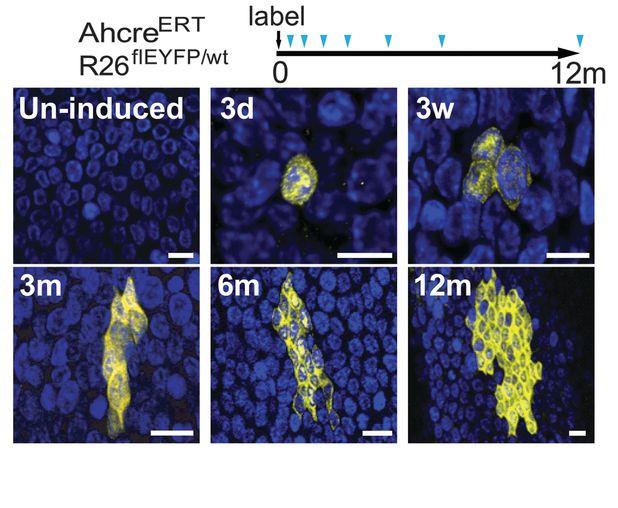
\includegraphics[width=0.5\textwidth]{oes-basal-pictures}
\par\end{centering}

\caption{\label{fig:oes-pictures}Protocol: Clonal labeling was induced in
genetically engineered mice and analyzed at intervals from 3 days
to 1 year (triangles). Images are rendered confocal z stacks of the
basal layer showing typical clones at times indicated. Enhanced yellow
fluorescent protein (EYFP), yellow; DAPI, blue. Scale bars, 10 $\mu$m.}


\end{figure}


In the work of {[}Clayton and Doup�{]}, such techniques were used
to show that the textbook {[}cite?{]} model of epithelial proliferative
units supported by a single long-lived, asymmetrically dividing stem
cell is at odds with the observed basal clone size distribution, and
that a stochastic model of progenitors dividing both symmetrically
and asymmetrically is capable of reproducing the experimental data.
We will engage in a similar analysis, and go further by establishing
a quantitative framework that allows precision measurement of relevant
quantities such as rate of turnover and proportions of progenitor
fate choice. We then use the method to analyse the action of a drug
(all-\emph{trans} retinoic acid) by quantitatively describing its
action on the fate outcome of the progenitors.

Of great biological significance, but relatively independent of the
analysis of clone size distributions, is the discovery that there
are no long-lived slow-cycling stem cells in the EE at all. As such,
the progenitors which we analyse in detail are also capable of repair,
by switching to a different pattern of behaviour. The reader interested
in these issues may find a discussion in {[}Doupe 2012{]}. This chapter
draws significantly on that publication, especially the supplementary
therein; the experimental work was performed by DPD, MPA and AR, project
planning by PHJ, thorough discussion with AMK, and data analysis by
GZ and BDS. PHJ wrote the main text of Ref {[}cite{]}, but section
2.2 is the authorship of BDS.

We will set out in detail the experimental evidence in support of
the esophageal progenitor (EP) cell model, how the parameters of this
model are constrained by the experimental data, and how the model
can be challenged experimentally by drug treatment. In section~\ref{sec:model}
we will describe how the experimental data identifies the dynamics
of a single progenitor cell population allowing us to formulate a
simple model of EE turnover. In section~\ref{sec:quant} we will
use the clonal fate data to fit the parameters of the modelling scheme.
Finally, in section~\ref{sec:chall}, we will challenge the model
by considering the effects of drug delivery on tissue.


\section{Clonal analysis: defining the model of EP cell dynamics\label{sec:model}}


\subsection{Scaling and equipotency}

\begin{figure}
\begin{centering}
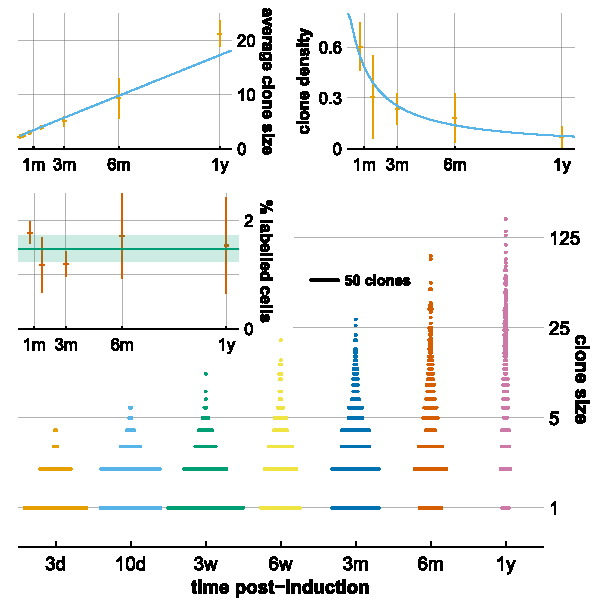
\includegraphics{basal-raw-gen}
\par\end{centering}

\caption{\label{fig:oes-basal-raw}\textbf{Main figure}: clone size distribution
(basal cells/clone) in a total of 1784 clones, each point represents
one clone. \textbf{Insets:} (top left and right) average basal clone
size and average density of clones in the basal layer, observed values
(orange) with error bars (mean \textpm{} SEM), blue curves show predictions
of model (\figref{oes-normal-model}). (middle left) average percentage
of labelled basal cells at indicated time points (orange), error bars
indicate mean \textpm{} SEM, green line and shading show average and
SEM across all time points.}


\end{figure}


To isolate and quantify the behavior of proliferating cells, we scored
the number of basal cells in clones containing two or more cells (i.e.
clones in which a proliferative cell was labeled at the start of the
experiment) from 3 days to one year post-induction, by confocal imaging
of esophageal wholemounts (fig). Previously, it has been shown that
in a similar homeostatic stratified squamous epithelium, interfollicular
epidermis, a simple statistical characterization can be used to both
establish the equipotency of a self-renewing cell population, and
elucidate the pattern of cell fate (cite 18, 19). In particular, if
self-renewal involves the stochastic loss and replacement of such
progenitors, clones derived from these cells will undergo a process
of ``neutral drift'' in which ongoing clonal loss is compensated
by the expansion of adjacent clones. However complex is the underlying
dynamics, such processes lead inexorably to the long-term scaling
of the surviving clone size distribution, in which the chance of finding
a clone with a size larger than some multiple of the average remains
constant over time.

\begin{figure}
\begin{centering}
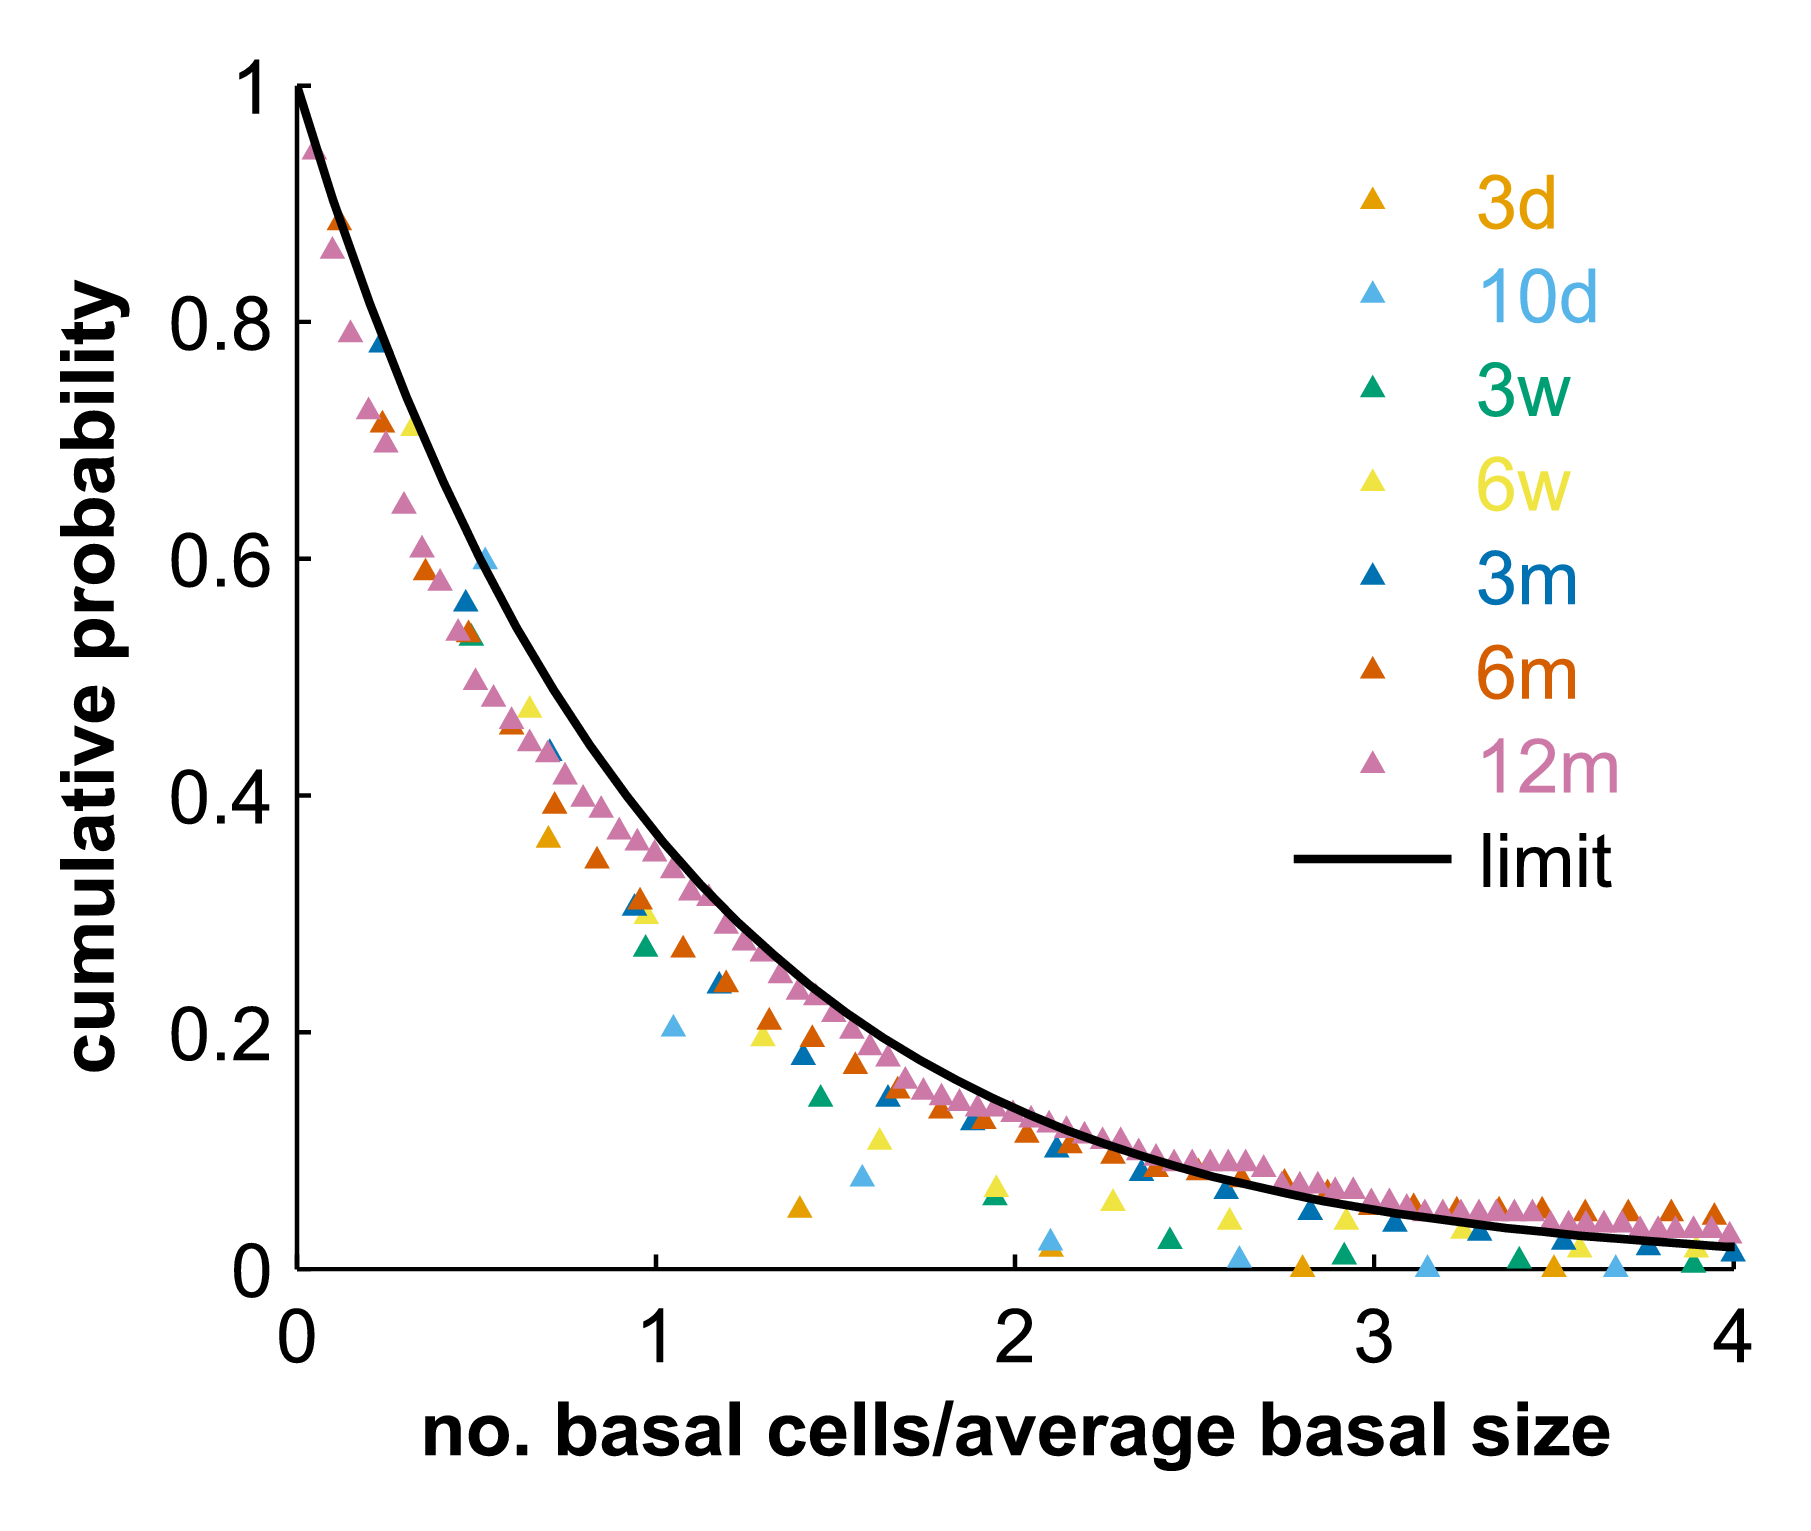
\includegraphics[width=0.5\textwidth]{basal-scaling}
\par\end{centering}

\caption{\label{fig:oes-basal-scaling}Cumulative clone size distribution shows
convergence onto scaling behaviour at late times. The raw basal layer
clone size distribution in (fig) is reproduced here as the cumulative
clone size distribution, $C_{n}(t)$, plotted as a function of $n$
divided by the average clone size for each timepoint. The cumulative
distribution $C_{n}(t)$ represents the probability of finding a surviving
clone with a basal layer size larger than $n$. At times of 3 months
or more post-induction, the data sets converge onto each other, a
manifestation of long-term scaling behaviour. Combined with the observed
homeostatic nature of the turnover, such scaling behaviour shows that
the self-renewing progenitor cells function as a functionally equivalent
population. The black curve denotes an exponential cumulative clone
size distribution; the long-term behaviour predicted for any strategy
involving population asymmetric self-renewal including the model discussed
here (1-2).}


\end{figure}


Applied to the current dataset, the convergence of the basal layer
clone size distribution onto a scaling form (\figref{oes-basal-scaling})
both confirms the functional equivalence of the self-renewing progenitor
cell population, and shows that the balance between their proliferation
and differentiation is achieved on a population basis, and not at
the level of individual cell divisions, i.e., in the course of turnover,
some cells may undergo terminal division leading to loss while others
may undergo symmetric duplication. Indeed, such behavior is consistent
with the observed heterogeneity in the clonal composition at short
times, which reveals that, soon after induction, all possible permutations
of two-cell clones can be found (i.e. two basal cells, one basal and
one suprabasal, and two suprabasal cells). The same degree of heterogeneity
is apparent in larger clones (\figref{oes-basal-raw}).

Taken together, the results above suggest that, as in interfollicular
epidermis, EE is maintained by a single cycling progenitor cell population
in which cell division can lead to all three possible fate outcomes;
two daughters that go on to divide, two cells that exit cycle and
then stratify out of the basal layer, or one daughter that goes on
to divide and one that differentiates (cite 18, 19). To assess the
validity of this model, and to quantify the respective rates and probabilities,
we must turn now to a more detailed analysis of the short-time data,
prior to scaling, where signatures of the detailed dynamics can be
elucidated. To prepare for this analysis, we must embed the progenitor
cell dynamics into a parameterization that includes the stratification
and loss of terminally differentiated cells.


\subsection{Parameterizing EP dynamics}

To be concrete, we will suppose that the basal layer comprises a single
population of cycling esophageal progenitor cells (with proportion
$\rho$), and their differentiating progeny (with proportion $1-\rho$),
which remain in the basal layer without dividing until they stratify.
If we assume that the progenitors divide with an average rate $\lambda$,
and the differentiating cells stratify at an average rate $\gamma$,
to achieve homeostasis, it follows that $\lambda\rho=(1-\rho)\gamma$,
i.e. the rate at which differentiated cells are generated in the basal
layer must be perfectly matched by the rate at which they stratify
into the suprabasal cell layer.

To further specify the model, we must also define the distribution
of cell cycle and stratification times. Here, for simplicity, we will
suppose that division and stratification are both uncorrelated between
successive events leading, in both cases, to an exponential (Poisson)
time distribution, with averages set by the rates $\lambda$ and $\gamma$,
respectively. While this assumption is surely unsafe (after all, cell
division must be accompanied by a small refractory period before further
division is possible), any degree of synchrony in the cell cycle or
stratification timings will be rapidly erased from the clonal record
over the timecourse. In particular, we expect features due to potential
synchrony to be lost within experimental error bars after ca. 1--2
rounds of division (cite 20).

Alongside the division and stratification rates, we must further specify
the probabilities for the respective fate outcomes following division.
Since both the labeled cell number and their composition is found
to be conserved over the time course, any process of cell division
must be consistent with homeostatic turnover. Moreover, since, through
scaling, EPs are seen to function as an equipotent cell population,
we will therefore suppose that proliferation and differentiation is
finely balanced so that, with probability, $r$, EP division results
in two dividing cells, with probability, $1-2r$, one dividing and
one non-dividing basal later cell, and with probability, $r$, two
non-dividing basal layer cells. Although we cannot rule out a small
contribution arising from perpendicular cell divisions resulting in
the placement of one of the daughters directly into the suprabasal
layer, given such divisions are observed to be rare, the effect of
such ``orientationally asymmetric'' divisions would again be impossible
to resolve. Similarly, we will neglect apoptosis, which was found
to be negligible in the basal layer (Fig. S4E).

In summary, the time-evolution of the basal layer population, along
with the clonal fate data, is therefore fully characterized by three
adjustable parameters, the division rate, $\lambda$, the stratification
rate, $\gamma$, and the fraction of divisions that lead to symmetrical
fate, $r$. The progenitor cell fraction is then fixed by the rates
$\rho=\gamma/(\lambda+\gamma)$. To fully characterize the behavior
of the \emph{total} clone size, including suprabasal as well as basal
cells, we must include a further parameter, $\mu$, which defines
the average rate at which suprabasal cells are shed from the tissue
(once again, we will suppose for simplicity that the corresponding
distribution of shedding times is Poisson). Fortunately, this additional
parameter can be related directly to the division and stratification
rates through the ratio of nucleated suprabasal to basal layer cells,
$m$, which can be measured directly. Then, since the ``flux'' of
differentiated cells stratifying from the basal layer must be perfectly
compensated by the flux of differentiated cells that are shed, we
must have $m\mu=\rho\lambda=\gamma\lambda/(\gamma+\lambda)$, thereby
providing a relation linking $\mu$ with $\gamma$ and $\lambda$.

Taken together, the EP cell model dynamics can be cast as a critical
(i.e. balanced) continuous time Markovian branching process, 
\begin{align*}
{\rm EP}\stackrel{{\displaystyle {\lambda}}}{\longrightarrow} & \left\{ \begin{array}{ll}
{\rm EP}+{\rm EP} & {\rm Pr.}\ r\\
{\rm EP}+{\rm T}_{{\rm B}} & {\rm Pr.}\ 1-2r\\
{\rm T}_{{\rm B}}+{\rm T}_{{\rm B}} & {\rm Pr.}\ r
\end{array}\right.\\
{\rm T}_{{\rm B}}\stackrel{{\displaystyle {\gamma}}}{\longrightarrow} & {\rm T}_{{\rm S}},\\
{\rm T}_{{\rm S}}\stackrel{{\displaystyle {\mu}}}{\longrightarrow} & \textrm{loss},
\end{align*}
where $\mathrm{EP}$ represents the progenitor, $\mathrm{T}_{\mathrm{B/S}}$
differentiated cells in the basal/suprabasal layer, and the rates
$\lambda$, $\gamma$, and $\mu$ are defined above. As discussed
above, we suppose that EP cell fate follows a pattern of intrinsic
or cell-autonomous regulation in which the fate outcome following
division is uncorrelated with the behavior of neighboring cells. In
previous studies, we have shown that, in the two-dimensional geometry
pertinent to EE, the long-term clonal dynamics is largely insensitive
to this choice (30).

This completes the specification of the cellular dynamics as a generalized
branching-type process. In principle, we could further refine the
modeling scheme to include aspects of the spatial regulation. However,
our aim here is to establish and challenge the simplest model which
is consistent with the observed range of clonal fate data. Indeed,
we will find that, by itself, this model provides a faithful description
of the cellular dynamics over the timecourse of the experiment. To
assess the integrity of the model, and to fit the three adjustable
parameters, we will make use of a Bayesian approach.


\section{Clonal analysis: quantitative modeling\label{sec:quant}}


\subsection{Scaling}

According to the EP cell paradigm, following induction, a differentiated
basal or suprabasal cell would progressively stratify, lose its cell
nucleus and be shed, providing only a transient contribution to the
clonal dynamics. By contrast, a clone derived from an EP cell would
progressively undergo chance expansion or contraction according to
the fate choice of the constituent cells. As tissue turns over, the
gradual extinction of some clones due to chance commitment to terminal
differentiation will be perfectly compensated by the expansion of
other clones. Analysis of the branching process shows that, over time,
neutral drift dynamics leads to a progressive (linear) increase in
the average size of the surviving clones, while the surviving fraction
falls proportionally such that the total density of labeled cells
remains constant (\figref{oes-basal-raw}, inset middle left) (18).
In this regime, the basal layer clone size distribution acquires a
scaling behavior (\figref{oes-basal-scaling}) described above. In
particular, the chance of finding a clone with more than $n$ basal
layer cells, takes the form of an exponential $\exp[-n/\langle n(t)\rangle]$
where, according to the parameters of the model, the average basal
layer clone size (i.e. the average size of the clone ``footprint''
on the basal layer) is given by $\langle n(t)\rangle\simeq t/\tau$
with $1/\tau=\rho/r\lambda$.

Although the long-term scaling behavior provides the means to extract
the characteristic timescale $\tau$ (see below), the rapid convergence
to this regime does not allow the individual parameters $\rho$, $r$,
and $\lambda$ to be inferred reliably from the basal layer clone
size distribution alone. Therefore, to properly validate the model,
and effect a reliable fit of the parameters, we consider the full
range of clonal fate data, short-term and long-term, basal and suprabasal.


\subsection{Parameter estimation}

The data itself is acquired in the form of a set of frequencies $D=\left\{ f_{bn}(t)\right\} $
describing the number of observations of clones with $b$ basal cells
and $n$ suprabasal cells at time $t$; an example is Fig. S6B. The
stochastic nature of our model will predict probabilities $p_{bn}(t)$
for a single cell to turn into a clone at time $t$ with $b$ basal
and $n$ suprabasal cells, based on the parameters $\rho$, $r$ and
$\lambda$. One might approach the fit with a least-squares method
to optimize the parameters. However, as a significant portion of our
data lies in the tails with large $b$ and $n$, where the counts
are small, we would have to employ complex methods such as ad-hoc
binning or continuity corrections. As such, we have elected to use
a more Bayesian approach, which allows us to analyze the experiment
with no manipulation of the data.

To fit the model to the range of experimental data, we implement a
basic algorithm involving Bayes' theorem for updating prior probabilities
in the presence of data. More precisely, the probability that the
observed clonal fate data $D$ is described by the model is specified
by the proportionality, 
\begin{eqnarray*}
P\left(\lambda,r,\rho|D\right)\propto P\left(D|\lambda,r,\rho\right)P\left(\lambda,r,\rho\right),
\end{eqnarray*}
where the posterior distribution $P(D|\lambda,r,\rho)$ denotes the
probability of obtaining the data $D$ given the parameters $\lambda$,
$r$, and $\rho$, multiplied by the likelihood that the parameters
are given by those same values. The constant of proportionality may
be calculated \emph{a posteriori} by imposing the normalisation, $\int_{0}^{\infty}\! d\lambda\int_{0}^{1}\! d\rho\int_{0}^{\frac{1}{2}}\! dr\, P\left(\lambda,r,\rho|D\right)=1$.
In our case, the posterior distributions will turn out to be approximately
Gaussian, so we may characterize the distribution by its first two
moments and treat them as a point estimate for the parameters, and
a credible interval covering approximately $68\%$ (using one standard
deviation) or $95\%$ (using two).

From Bayes' equation above, it is apparent that we need to specify
a prior distribution $P\left(\lambda,r,\rho\right)$ and a likelihood
function $P\left(D\middle|\lambda,r,\rho\right)$. We chose the maximum
entropy prior as we have no further cogent information, which corresponds
to $\rho$ uniform on the interval $[0,1]$, $r$ uniform on the interval
$\left[0,\frac{1}{2}\right]$, and $\lambda$ log-uniform. Crucially,
since we have sufficient data, the likelihood function is sharply
peaked and only significant on a small support, and thus the posterior
distribution is dominated by the likelihood function, and so any reasonable
prior (one which does not fluctuate strongly over that narrow support)
would give quantitatively similar results.

Turning to the likelihood function, since each observed clone is independent,
it is a multinomial distribution with a countable number of outcomes:
\[
P\left(D\middle|\lambda,r,\rho\right)=\prod_{t}\frac{\left[\sum_{bn}f_{bn}(t)\right]!}{\prod_{bn}\left[f_{bn}(t)!\right]}\prod_{bn}\left[p_{bn}(t)\right]^{f_{bn}(t)},
\]
where $p_{bn}(t)$ denote the expected probabilities that a clone
contains $b$ basal cells and $n$ suprabasal cells at time $t$ post-induction.
In the following, we will suppress the time index $t$ for notational
concision where it is considered unambiguous. To eliminate potential
ambiguities due to uncertain induction frequencies of the two cell
types, we conditioned the data on having at least two cells, which
removes the events where a differentiated cell is induced. Moreover,
to focus on a defined population, we further consider only clones
which retain at least one basal layer cell. Thus we consider the probabilities,
\[
p_{bn}\mapsto\tilde{p}_{bn}=\begin{cases}
0 & b=0\textrm{ or }b+n<2,\\
\frac{p_{bn}}{1-p_{10}-\sum_{n}p_{0n}} & \textrm{otherwise.}
\end{cases}
\]


To determine the probabilities $p_{bn}$, we consider the more fundamental
distribution $p_{lmn}$ describing the (unconditioned) probability
of finding a clone with $l$ progenitors, $m$ differentiated basal
layer cells and $n$ suprabasal cells. From these probabilities we
can determine $p_{bn}$ through the relation, $p_{bn}=\sum_{l+m=b}p_{lmn}$.
The probabilities $p_{lmn}$ obey a continuous time Markov process,
with the time-evolution given by the Master equation, 
\begin{align*}
\frac{d}{dt}p_{lmn} & =\lambda\left[r(l-1)p_{(l-1)mn}+(1-2r)lp_{l(m-1)n}+r(l+1)p_{(l+1)(m-2)n}-lp_{lmn}\right]\\
 & +\gamma\left[(m+1)p_{l(m+1)(n-1)}-mp_{lmn}\right]-\mu np_{lmn}.
\end{align*}
with the initial conditions $p_{lmn}=\delta_{l1}\delta_{m0}\delta_{n0}$.

Although this is a straightforward set of coupled differential equations,
direct numerical solution is prohibitively computationally expensive
because each element is coupled to all the others: attempts to truncate
the $lmn$-space causes errors that are hard to control. Instead,
to develop the computational scheme, it is helpful to package the
equations into the form of a generating function, $G(x,y,z,t)=\sum_{lmn}p_{lmn}(t)x^{l}y^{m}z^{n}$,
which obeys the differential equation, 
\begin{align*}
\frac{\partial G}{\partial t} & =\lambda\left[rx^{2}+(1-2r)xy+ry^{2}-x\right]\frac{\partial G}{\partial x}+\gamma\left(z-y\right)\frac{\partial G}{\partial y}+\mu(1-z)\frac{\partial G}{\partial z},\\
 & =\lambda\left[f_{x}(x,y,z)-x\right]\frac{\partial G}{\partial x}+\gamma\left[f_{y}(x,y,z)-y\right]\frac{\partial G}{\partial y}+\mu\left[f_{z}(x,y,z)-z\right]\frac{\partial G}{\partial z}.
\end{align*}
with $G(x,y,z,t=0)=x$ and 
\begin{align*}
f_{x}(x,y,z) & =rx^{2}+(1-2r)xy+ry^{2},\\
f_{y}(x,y,z) & =z,\\
f_{z}(x,y,z) & =1
\end{align*}
which can be recognised as the probability generating functions for
individual divisions of each cell type.

The partial differential equation for $G$ may be solved by the method
of characteristics. Introducing the auxiliary equations, 
\[
\frac{\partial}{\partial t}F_{v}(\mathbf{v},t)=a_{v}\left[f_{v}\left(F_{x},F_{y},F_{z}\right)-v\right]
\]
where $\mathbf{v}=(x,y,z)$, $v$ ranges over the set $\{x,y,z\}$,
$a_{v}$ ranges over $\{\lambda,\gamma,\mu\}$ and $F_{v}(\mathbf{v},t=0)$
ranges over $\{x,y,z\}$, we can write the solution to $G$ as $G(x,y,z,t)=F_{x}(x,y,z,t)$.
In fact, we can recognize the auxiliary function $F_{v}$ as the probability
generating functions for the clone size distribution starting with
a cell of type $v$.

Finally, the coefficients $p_{lmn}$ may be extracted from $G$ by
complex analysis. Indeed, it is possible to directly extract $p_{bn}$
by considering $G(x,x,z,t)$. Defining 
\[
H(x,y,t)=G(x,x,y,t)=\sum_{bn}p_{bn}(t)x^{b}y^{n},
\]
we see that $H$ is analytic in both $x$ and $y$ on the complex
unit disc $|x|,|y|\le1$, and so there are no poles within it. Defining
$\mathcal{C}$ to be an anticlockwise contour around the unit circle,
we can recover $p_{bn}$ by considering residues at zero: 
\[
p_{bn}(t)=\left(\frac{1}{2\pi i}\right)^{2}\oint_{\mathcal{C}}dx\oint_{\mathcal{C}}dy\frac{H(x,y,t)}{x^{b+1}y^{n+1}}.
\]
Note that, up to a minus sign, it is just a multi-dimensional inverse
$Z$-transform. The integral can be approached by a sum 
\[
p_{bn}(t)=\lim_{M\rightarrow\infty}\sum_{j=1}^{M}\sum_{k=1}^{M}H\left(e^{2\pi ij/M},e^{2\pi ik/M},t\right)e^{-2\pi ijb/M}e^{-2\pi ikn/M}
\]
the truncation of which at finite $M$ approximates the integral and
is in the form of a two-dimensional discrete Fourier transform. This
allows the use of industrial Fast Fourier Transforms to evaluate all
$p_{bn}$ for $M$ being a power of two simultaneously. We use adaptive
oversampling to estimate the error in the truncation, and use it to
bound the errors. This gives a robust black box algorithm which gives
point estimates and credible intervals for arbitrary clonal data sets.

Before finally carrying out the parameter estimation, it is important
to confirm that the degree of inter-mouse variation is sufficiently
small to justify collating data from different mice. For this purpose,
we made use of the long-term scaling behaviour of the clone size distribution.
Although, generically, the dynamics of the basal layer cells depends
independently on the three adjustable parameters, $\rho$, $\lambda$
and $r$, in the scaling limit, the basal layer clone size depends
only on the only on the combination, $1/\tau=r\lambda/\rho$, a measure
of the rate of progenitor cell loss and replacement. As a result,
this parameter can be estimated with a smaller uncertainty, allowing
it to be inferred on a mouse by mouse basis for each timepoint. Inferring
this parameter from the basal layer clone size distribution, as well
as the total clone size at shorter times, the comparison shown in
\figref{oes-intermouse} reveal that, although there is some degree
of inter-mouse variation, the amalgamation of data from different
mice at the same timepoint can be justified.

\begin{figure}
\begin{centering}
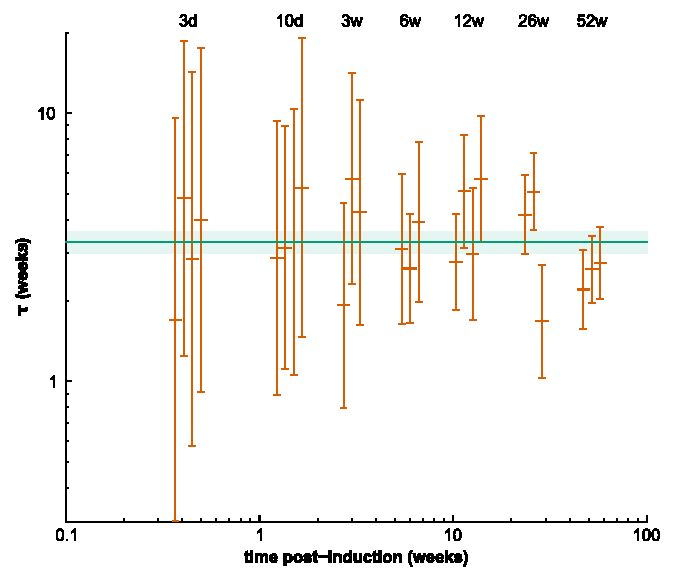
\includegraphics{intermouse-tau-basal}
\par\end{centering}

\begin{centering}
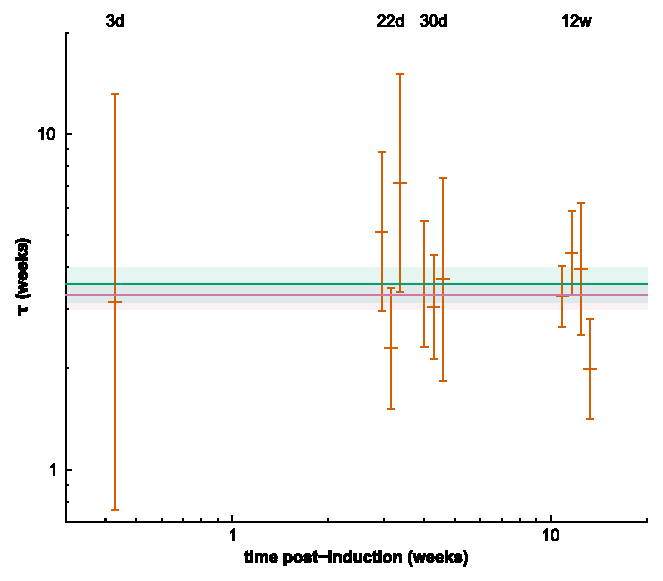
\includegraphics{intermouse-tau-normal}
\par\end{centering}

\caption{\label{fig:oes-intermouse}\textbf{Upper}: from the data from each
mouse, we can separately estimate the combined parameter $\tau=\rho/r\lambda$.
On the left, we plot $\log(\tau)$ with 68\% ($1\sigma$) credible
intervals for 28 mice using the basal clone size distribution, along
with the combined average (and $1\sigma$ credible interval) in green
from treating all mice as exactly identical. \textbf{Lower}: we use
the full (basal and suprabasal joint distribution) from 11 mice, with
the combined average in purple, and the average from the left figure
in green.}


\end{figure}


\begin{figure}
\begin{centering}
\includegraphics[width=0.3\textwidth]{oes-F2\lyxdot large}
\par\end{centering}

\caption{\label{fig:oes-normal-model}Basal layer comprises 65\% functionally
equivalent EP (green, dividing at a rate of 1.9/week) and 35\% postmitotic
cells (pink), which stratify (arrow) at a rate of 3.5/week. Ten percent
of EP divisions generate two EP daughters, 10\% two differentiated
daughters, and 80\% one of each fate. Values are point estimates with
95\% plausible intervals.}


\end{figure}


Using the full clone data (\figref{oes-basal-raw} and \figref{oes-joint-data})
we computed a posterior distribution on $\rho$, $\lambda$ and $r$.
This distribution is narrow and Gaussian-like, so we can describe
it using its first two moments. Specifically, the mean is a point
estimate for the parameters, and twice the standard deviation is an
estimate for the $95\%$ credible interval; the results are shown
in (\figref{oes-normal-model}). We show a comparison between the
fitted parameters and the detailed basal and suprabasal cell number
distribution in \figref{oes-joint-data}. We used the point estimates
to computed a set of probabilities, with which we can compute $95\%$
likelihood intervals for $f_{bn}$ knowing the total number of clones
observed (which we have called plausible intervals due to a lack of
standard nomenclature); these are plotted as the error bars in the
model, and the graphs form a visual significance test with the null
hypothesis being the model with the parameters as estimated. We draw
attention to the fact that these do not contain the uncertainties
in the parameters themselves. Furthermore, \figref{oes-basal-comparison}
contains a detailed comparison with the much larger basal clone size
data set, which shows the expected deviations from scaling at shorter
times; again the error regions refer to the sampling error only. Lastly,
the insets in \figref{oes-basal-raw} show the comparisons with density
and average size of basal clones; the error bars in are the mouse
to mouse variation. Given that we can fit the entire distributions
at all times the average size also fits (unsurprisingly). However
it should be noted that we can make a prediction of the density which
fits within the experimental error, with only one parameter, the induction
efficiency, estimated by the labelling frequency at time zero.

\begin{figure}
\begin{centering}
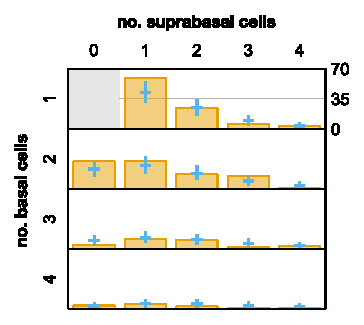
\includegraphics{normal-22-days}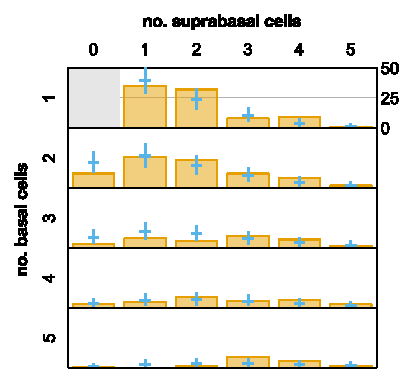
\includegraphics{normal-30-days}
\par\end{centering}

\begin{centering}
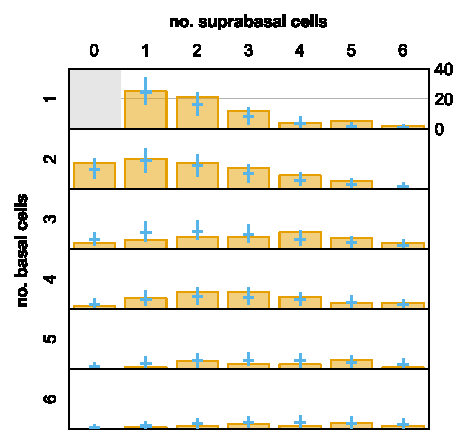
\includegraphics{normal-12-weeks}
\par\end{centering}

\caption{\label{fig:oes-joint-data}Joint clone size distribution of clones
containing at least one basal cell and two cells in total at 22, 30
and 84 days post-induction; orange bars show raw counts, blue crosses
show model predictions using point estimates for parameters from \figref{oes-normal-model}
with $95\%$ plausible intervals.}


\end{figure}


\begin{figure}


\centering{}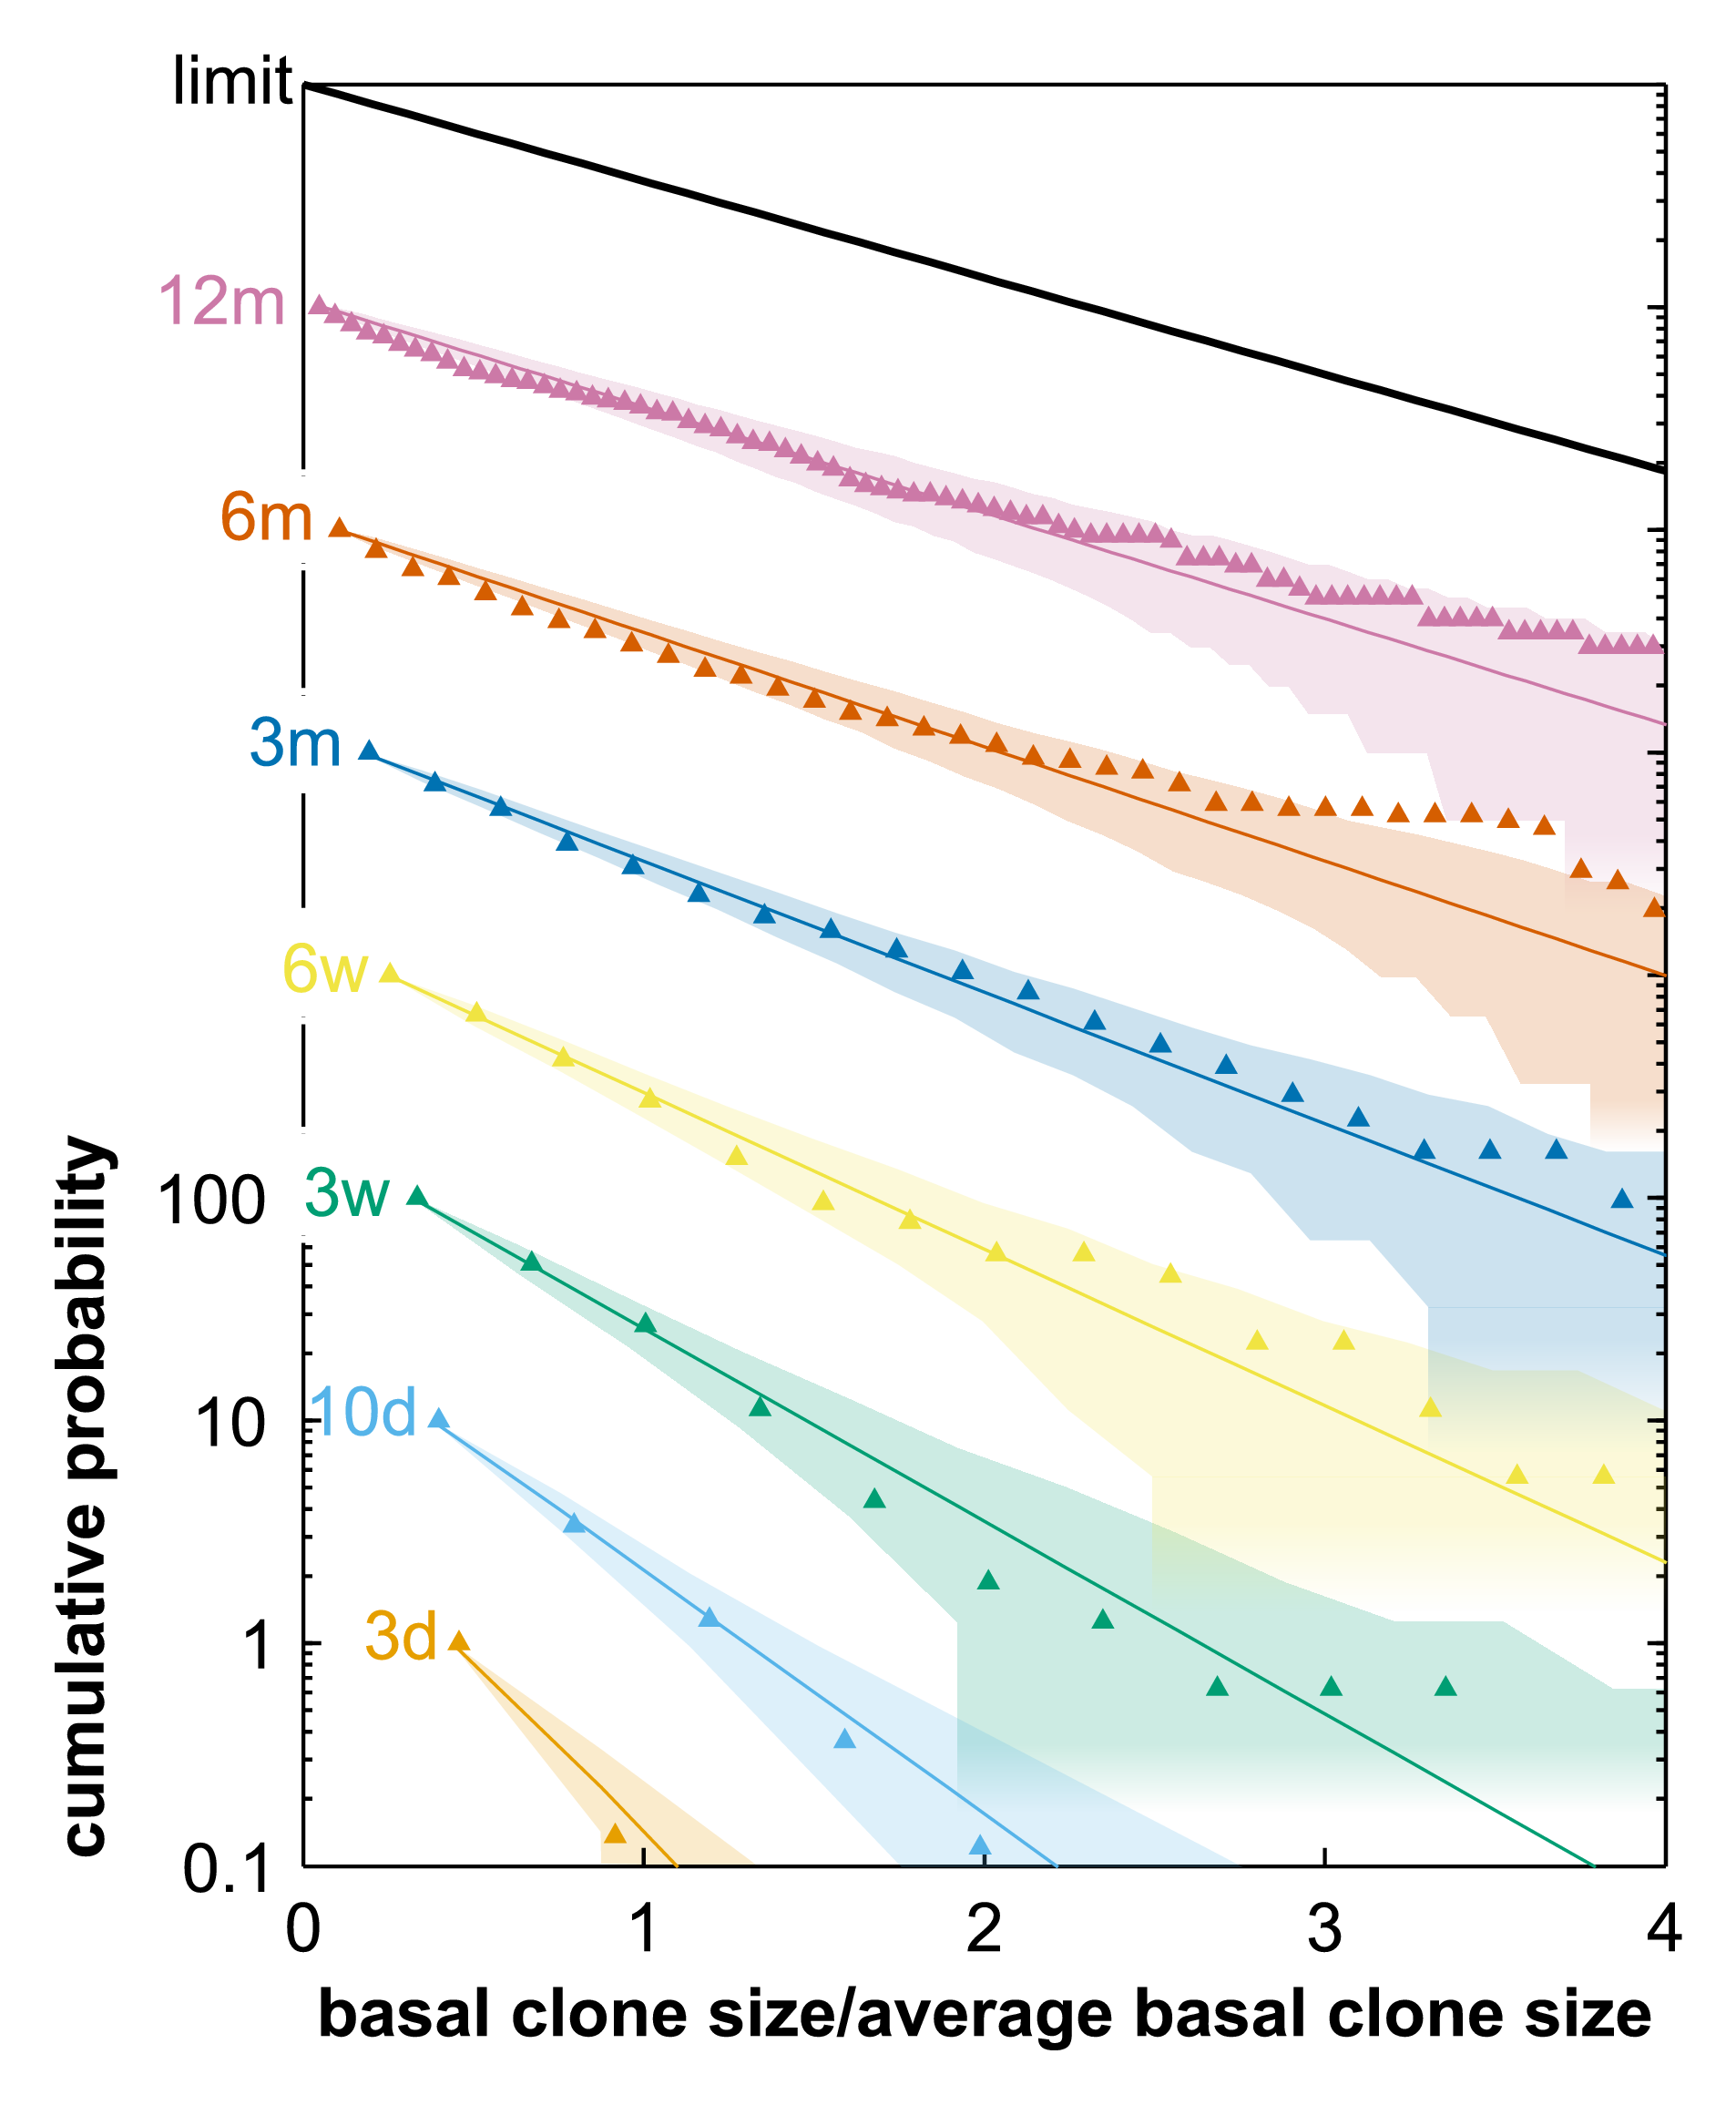
\includegraphics{basal-comparison}\caption{\label{fig:oes-basal-comparison}: Cumulative basal layer clone size
distribution, $C_{n}(t)$, as a function of size (number of cells)
rescaled by the average for each time point, $n/\langle n(t)\rangle$
as in \figref{oes-basal-scaling}, i.e. $C_{n}(t)$ denotes the probability
of finding a clone with a size equal to, or larger than, $n/\langle n(t)\rangle$.
Here we have presented the cumulative probability distribution on
a logarithmic scale and, for clarity, we have separated consecutive
time points by one decade. The points denote experimental data from
main part of \figref{oes-basal-raw}, and the lines represent the
corresponding model predictions using point estimates from \figref{oes-normal-model}.
The shaded regions represent estimates of the stochastic error due
to finite sample size, indicating approximately one standard deviation
($68\%$). In the long time limit, the model predicts that the distribution
should tend to a simple exponential, $\exp\left(-n/\langle n(t)\rangle\right)$,
(black line). The model shows good agreement with the experimental
data at both short and long time points.}
\end{figure}



\section{Clonal analysis: challenging the model\label{sec:chall}}


\subsection{Effects of atRA treatment}

It is straightforward to implement the same inference algorithm to
address the atRA treated tissue. Wit the assumption that atRA pre-treatment
establishes a new steady-state EP cell dynamics, the resulting fit
of the model to the experimental data is shown in \figref{oes-atra-model},
while the resulting model predictions are shown alongside the experimental
data in \figref{oes-atra-homeo}. Once again, the fits reveal a close
agreement of the model with the experimental data.

\begin{figure}
\begin{centering}
\includegraphics[width=0.3\textwidth]{oes-F3\lyxdot large}
\par\end{centering}

\caption{\label{fig:oes-atra-model}During atRA treatment, proliferation and
differentiation rates (red) increase compared with control, whilst
no significant changes occur to progenitor fate choice.}


\end{figure}


\begin{figure}
\begin{centering}
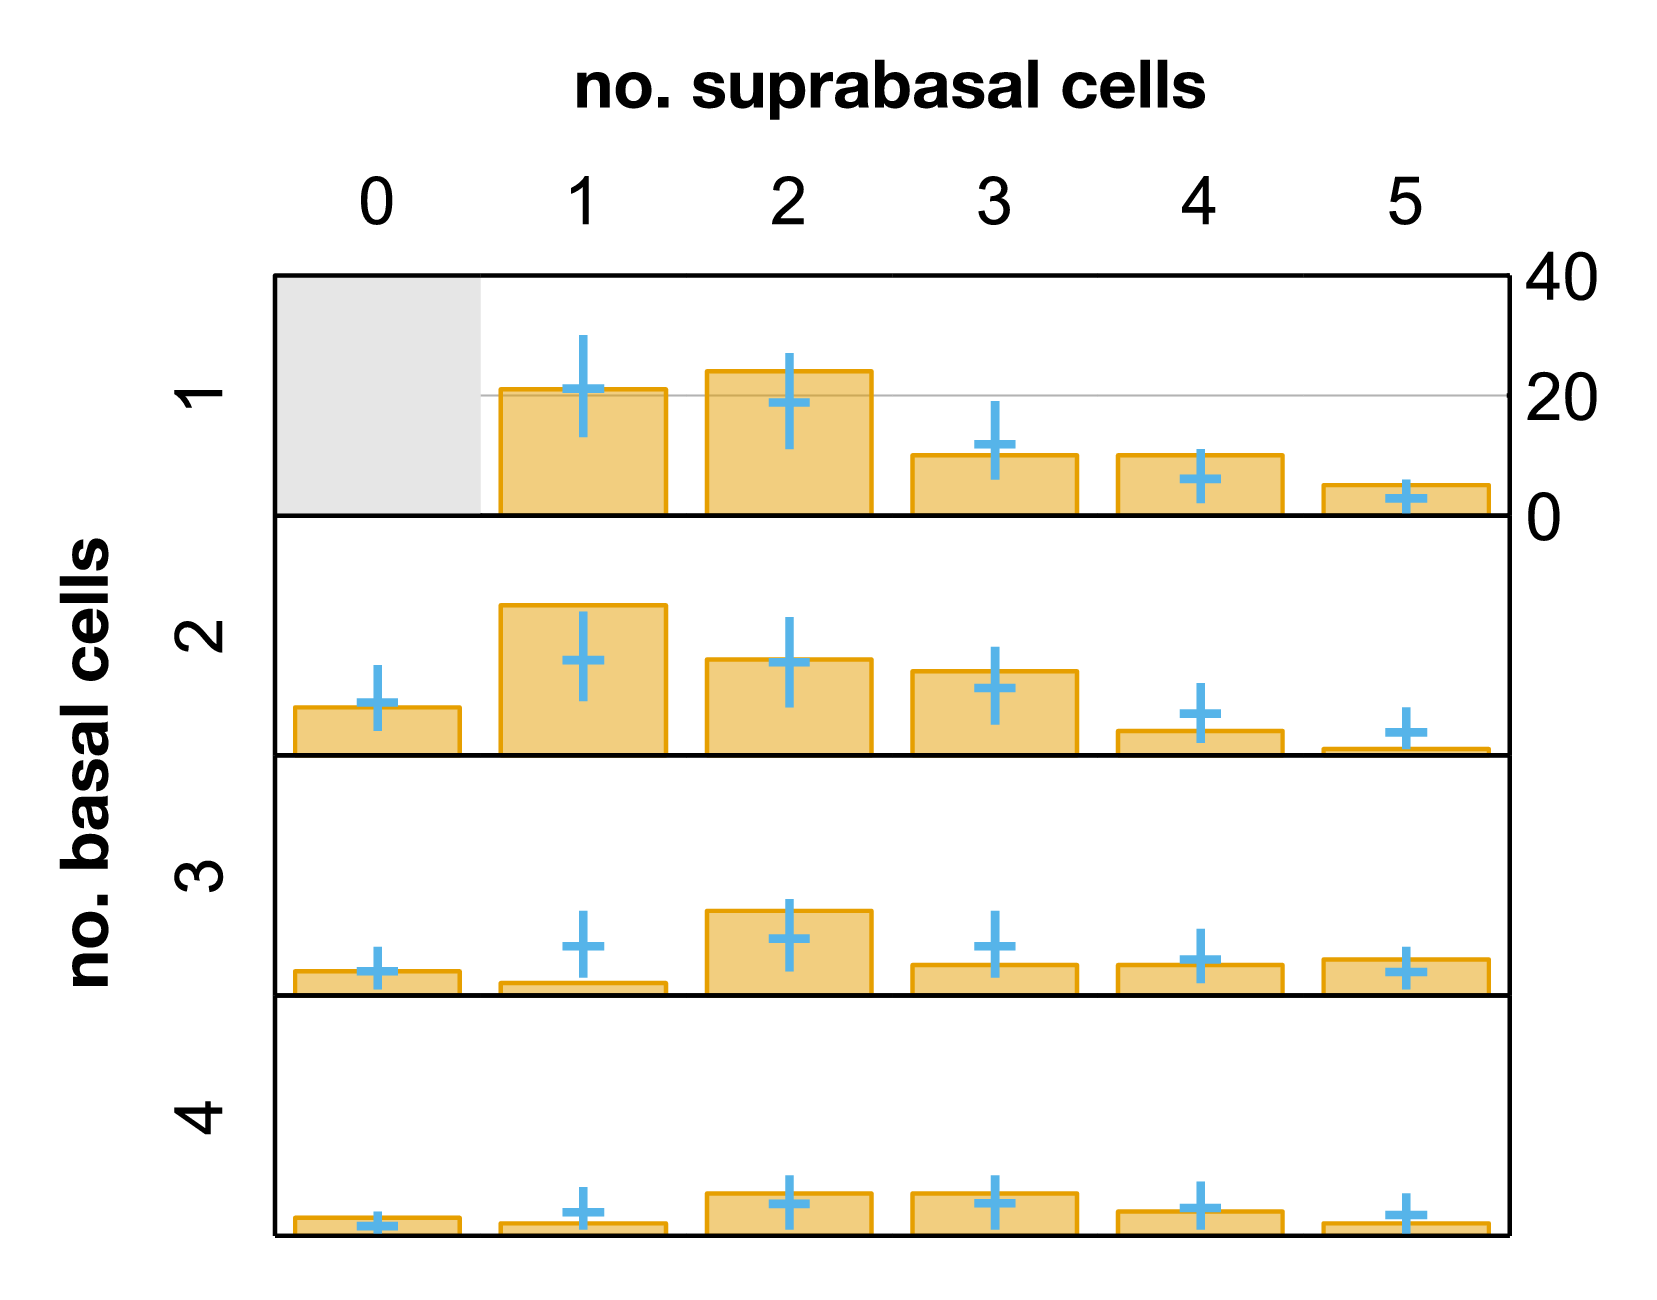
\includegraphics{atRA-homeo-3-weeks}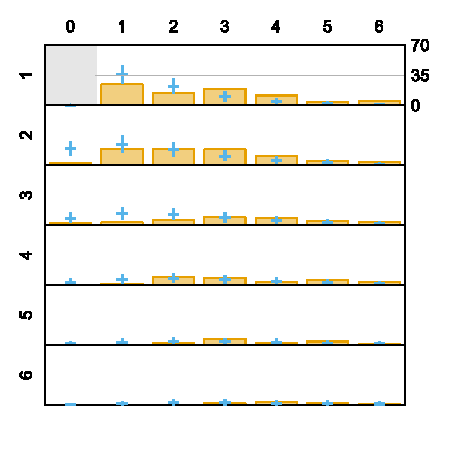
\includegraphics{atRA-post-30-days-joint}
\par\end{centering}

\caption{\label{fig:oes-atra-homeo}Similar to \figref{oes-joint-data}, the
raw data and model fits for atRA under homeostatic conditions, at
3 and 6 weeks post-induction.}


\end{figure}


With the parameters for normal and atRA treated tissue in hand, it
is then possible to predict the outcome when atRA is applied after
induction. In particular, if we assume that, following atRA treatment,
the division and stratification rates immediately adjust from their
normal to atRA treated steady-state values, we can predict the resulting
clone dynamics. Indeed, when compared to the measured basal clone
distribution, we find that the predictions offer a favourable fit
(\figref{oes-atra-jump}, left). By contrast, comparison with the
joint suprabasal and basal distribution shows significant deviations
(\figref{oes-atra-jump}, right). This departure can be easily understood
as the effect of atRA treatment on cells which have already stratified
and left the basal layer is more complex, and there may be some time-lag
before the entire tissue changes to the new steady-state behavior.
Nevertheless, these results suggests that, as far as the basal layer
is concerned, the application of atRA treatment can be well-approximated
as an instantaneous change of the parameters of the EP cell dynamics.

\begin{figure}
\begin{centering}
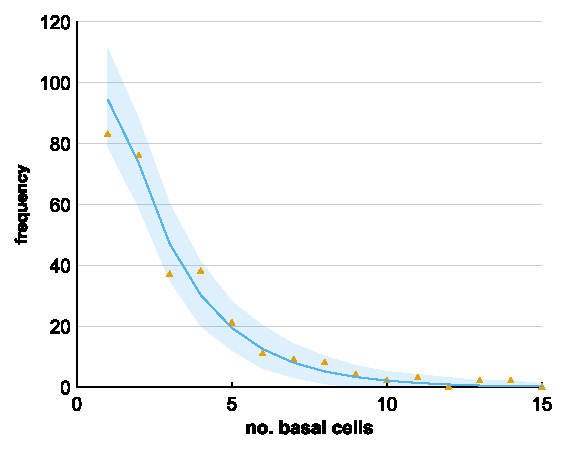
\includegraphics[width=0.5\columnwidth]{atRA-posttreat-30-days}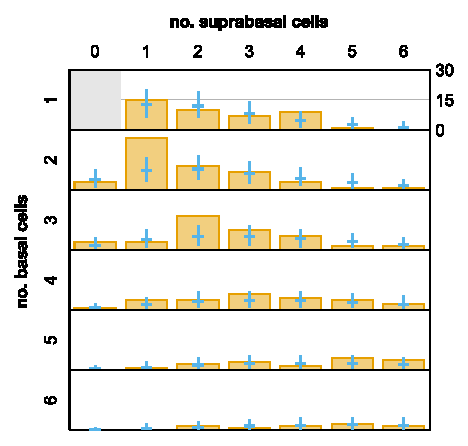
\includegraphics[width=0.5\columnwidth]{atRA-homeo-6-weeks}
\par\end{centering}

\caption{\label{fig:oes-atra-jump}\textbf{Left}: number of basal cells per
clone in EE treated by applying atRA for 9 days, starting 3 weeks
post-induction: orange triangles indicate experimental data, blue
line indicates prediction of model (instantaneous change from model
in \figref{oes-normal-model} to model in \figref{oes-atra-model})
shown with $95\%$ plausible intervals. A total of $316$ clones were
scored in 3 mice. \textbf{Right}: joint clone size distribution of
the same 316 clones, in orange. The blue crosses show the prediction
of the model represented with the 95\% plausible interval indicated
by vertical blue bars.}


\end{figure}



\subsection{Single cell clones}

Finally, the development of the EP model relied upon the observation
of long-term scaling behavior of the basal layer clone size distribution
which suggested that tissue maintenance involves only a single equipotent
progenitor cell population. However, by focusing on clones with a
total size greater than one, we eliminated the potential signature
of a second very slow-cycling or quiescent cell population. Although
the existence of such a population in EE was ruled out by the H2B-GFP
assay, with the predictions of the EP model, we can do back and question
whether the dynamics of the single-cell clones are consistent with
the ansatz of the modeling scheme.

Since, for times in greatly in excess of the cell stratification time,
$1/\gamma$, differentiated cells labeled at induction will have been
lost from the basal layer, we can use the long-term evolution of the
single-cell basal clones to challenge the predicted model dynamics.
Once again, the results, shown in Fig. S13, reveal an excellent agreement
between theory and experiment over the year long timecourse. In particular,
we can conclude that the persistence of single-cell clones merely
reflects the set of clones which, by chance, have expanded and the
sister cells have been shed leaving behind a single labeled cell.

\begin{figure}
\begin{centering}
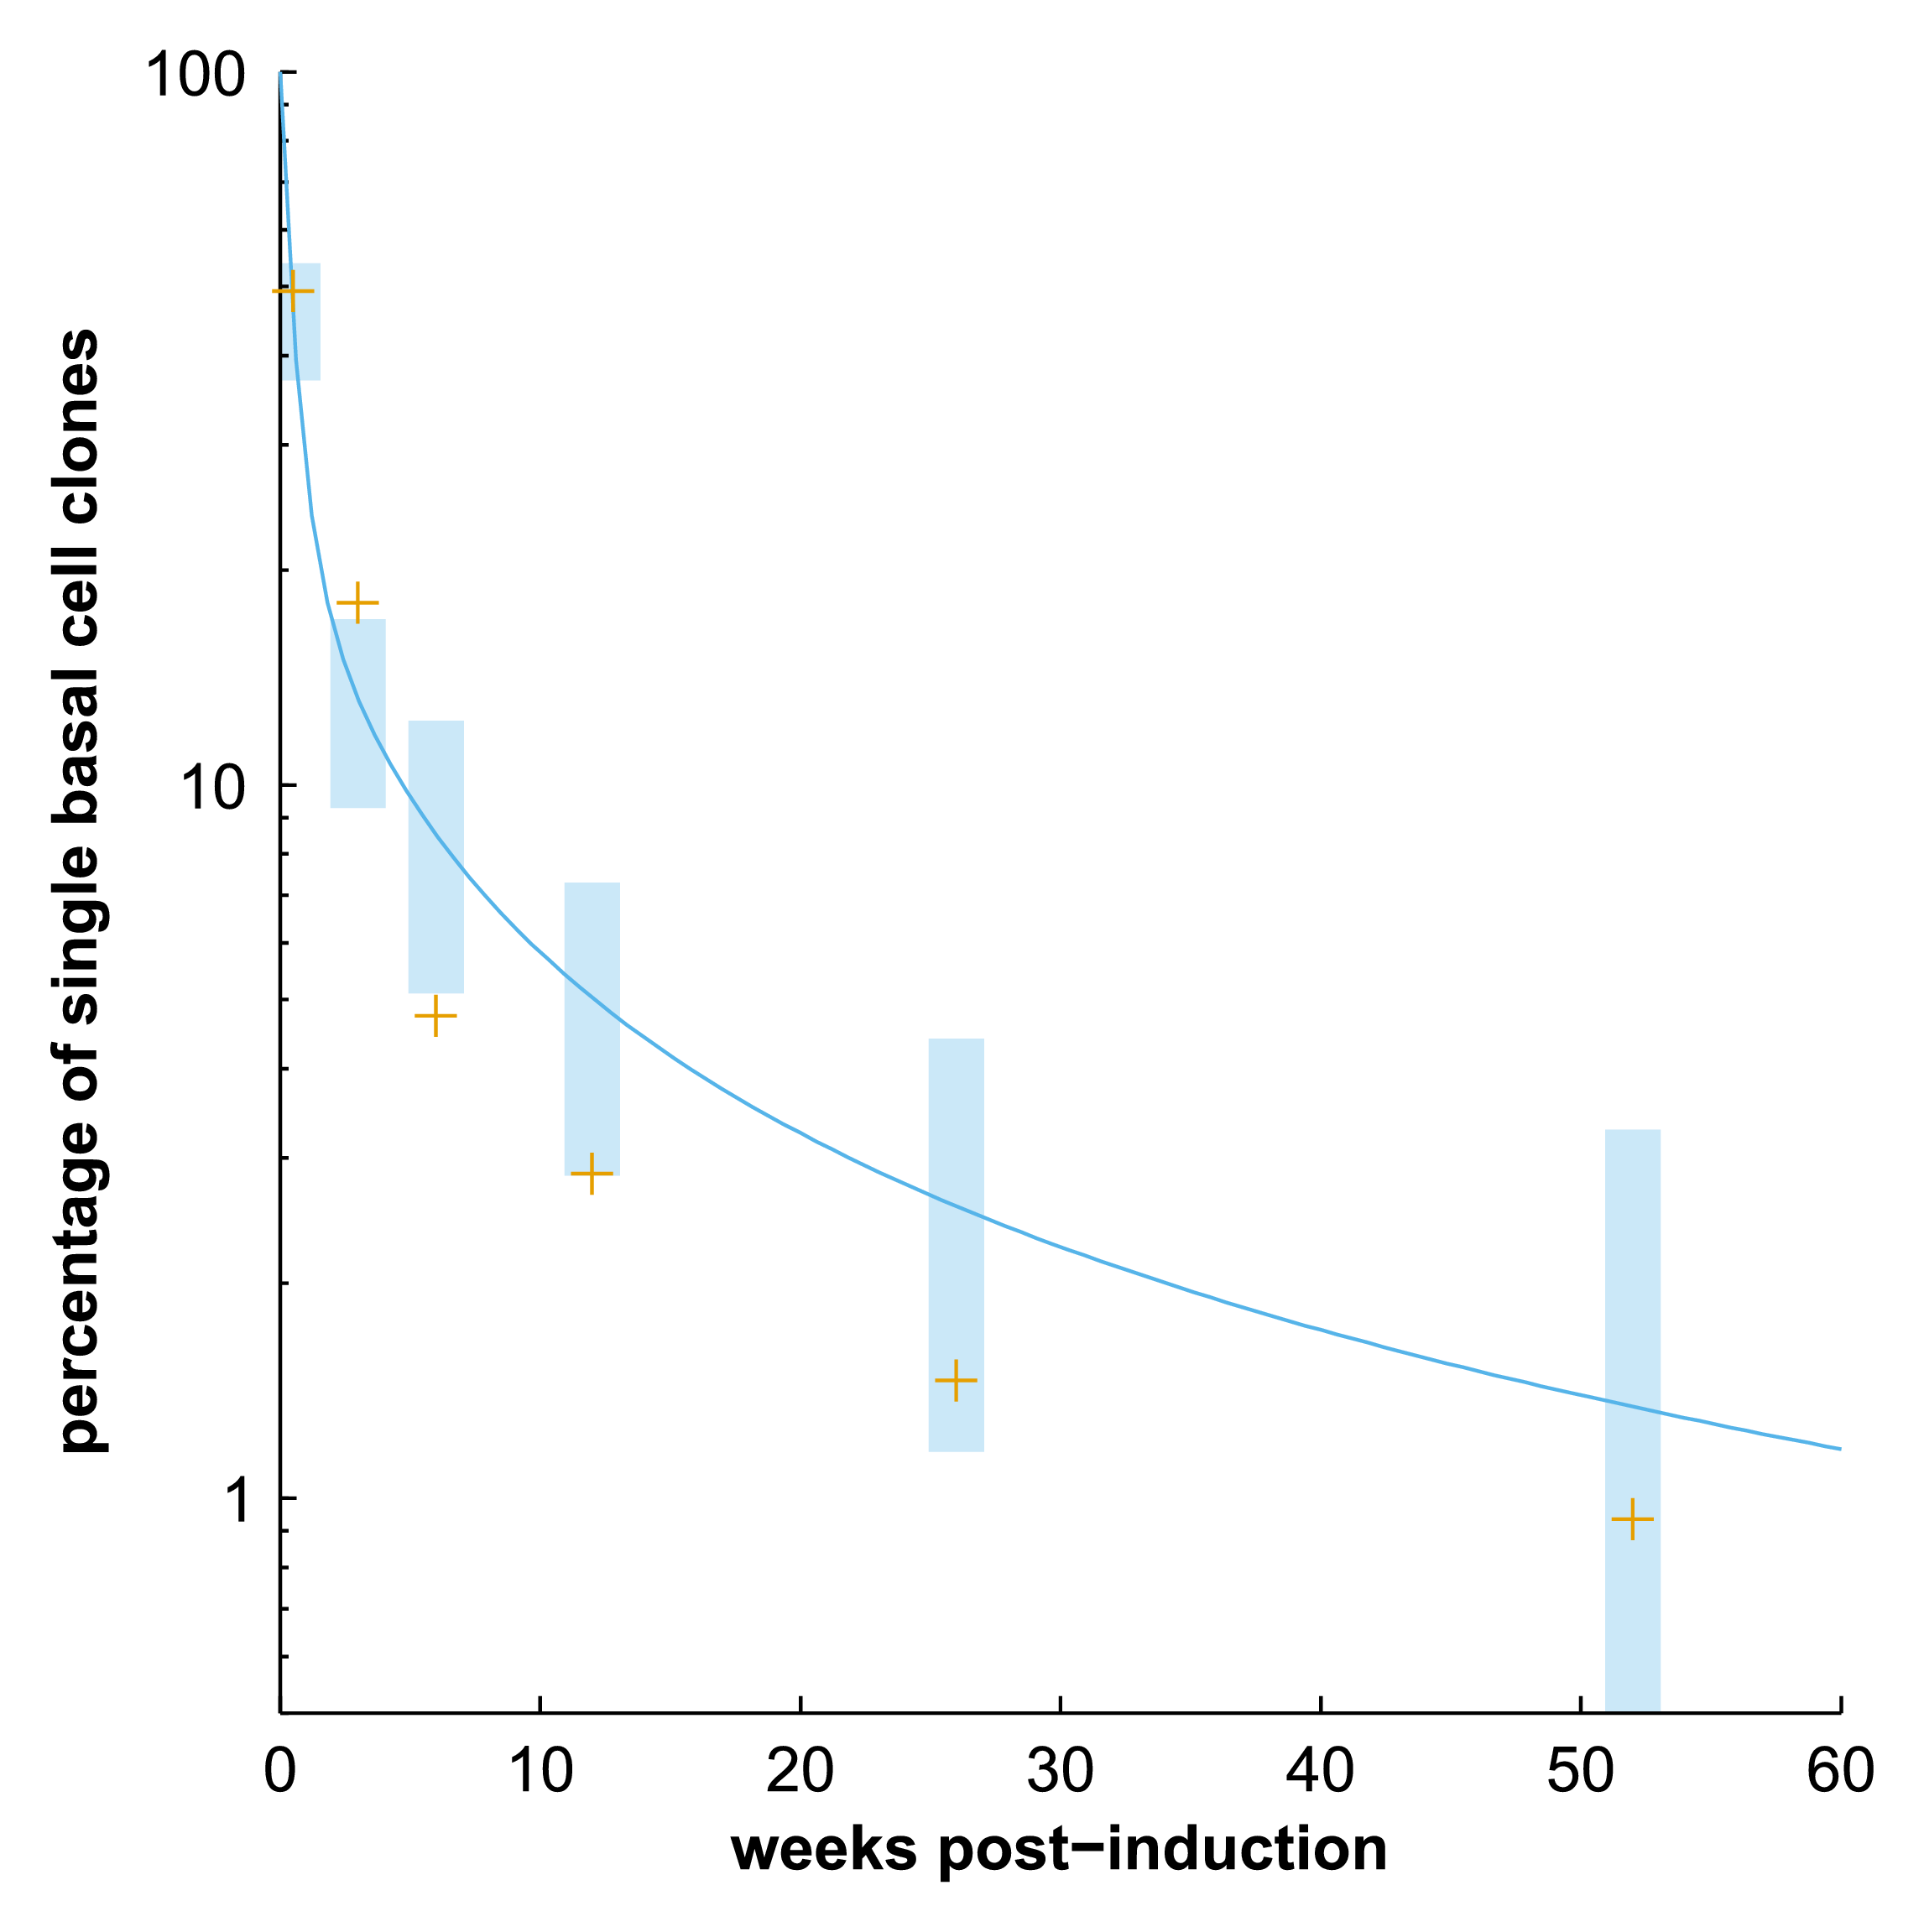
\includegraphics{singles}
\par\end{centering}

\caption{\label{fig:oes-single-cell}There is a very slow decay of the relative
frequency of clones consisting of a single basal cell. Nevertheless,
this is well accounted for by the model (Fig. 2F). Here we plot the
observed relative frequency in orange, and in blue the model prediction
(with 95\% likelihood intervals arising from finite number of clones
counted).}


\end{figure}



\section{Conclusion}

We have shown that there is a population of progenitors in EE which
maintains the tissue, which is modelled by a simple stochastic branching
process. The progenitors divide at a constant rate and chose one of
three fates with fixed probabilities; differentiated cells stratify
and eventually shed. The model contains four parameters: the EP cell
division rate $\lambda$, the ratio of symmetric to asymmetric cell
divisions controlled by the parameter $r$, the stratification rate
$\gamma$, and the loss rate of cells from tissue $\mu$. The latter
is fixed by the ratio of basal to suprabasal cells, which may be accurately
measured; the other three were measured from observed clone size distributions.
Moreover, we have shown that this model can capture the effect of
atRA treatment through a straightforward adjustment of the average
EP cell division rate.


\chapter{Theorems on Super-critical Branching Processes}

When cancer cell lines are cultured, it is sometimes observed that
all cells remain in cell cycle (according to biochemical markers).
It therefore seems reasonable to model the cells as independent and
identical, which has a natural expression in the theory of super-critical
branching processes \cite{Athreya2004}. Furthermore, as the cells
proliferate rapidly, it is possible to obtain some fairly large amount
of statistics regarding the clone size distribution. It is well-known
that the limit distribution depends on the lifetime distribution of
the particles, i.e. the cell cycle distribution. We therefore seek
to infer the cell cycle distribution from the measurable clone size
distribution. Concretely, we attempt to invert the relationship between
the cell cycle distribution and the clone size distribution, and investigate
its stability and (un)suitability as a practical procedure. Along
the way we find that not all distributions can arise as the limiting
distribution of a super-critical branching process, and we conjecture
and prove some properties of them. 

This chapter was inspired by conversations with the Jones team, who
provided the initial data for this theoretical detour. It is unfortunate
that ultimately the results were not sufficiently useful to be biologically
relevant.


\section{The inversion formula}

Consider an equipotent population of cells which divide independently.
This may be modelled as a branching process, defined by specifying
the cell cycle distribution be $g(t)$ and the branching outcomes
of each division, which we package into a generating function $f(s)=\sum_{k}p_{k}s^{k}$
where $p_{k}$ is the probability for the cell to divide into $k$
daughters. We will restrict ourselves to biologically feasible processes,
in particular we will require all moments of $f$ to exist. Furthermore,
we will assume that $p_{0}=0$, as it simplifies the consideration
by avoiding total death of the clone; for any given $f$ we can construct
a $f^{\star}$ of equal order such that no death occurs, with the
only difference being the existence of terminal clones (see appendix\ref{app:condition-survival}).
We also exclude certain pathological behaviours from consideration,
such as the possibility for a clone to reach infinite size in finite
time, which excludes in particular the existence of a Dirac delta
spike at zero in $g$. We consider in particular the \emph{super-critical}
process, where $f^{\prime}(1)>1$ and the expected number of cells
diverges exponentially at a rate $\alpha\left[f,g\right]$ (the Malthusian
parameter of the process), defined by the (only) root of 
\[
f^{\prime}(1)\int_{0}^{\infty}e^{-\alpha y}g(y)\, dy=1.
\]
 In the limit of infinite time, the distribution (normalised to unit
mean) of the total number of cells converges to a distribution $H(W)$,
whose characteristic function $\phi(u)=\mathbb{E}\left[e^{iuW}\right]$
is the unique solution (amongst distributions with unit mean) of
\begin{equation}
\phi(u)=\int_{0}^{\infty}f\left[\phi\left(ue^{-\alpha y}\right)\right]g(y)\, dy.\label{eq:forwards-eq}
\end{equation}
Notice that since the constant $\alpha$ sets a scale for $g$, we
may remove it by scaling $g$ with no change to the limiting behaviour.
Therefore without loss of generality we shall set $\alpha=1$.

We can consider equation \ref{eq:forwards-eq} as a family of non-linear
transform on the space of distributions over the positive reals, indexed
by the generating function $f$. It We note two properties (see appendix
\ref{app:injective-continuity}) in particular: it is continuous (in
$l_{1}$-norm), and injective (for a fixed $f$, up to scaling of
$g$). In particular, this implies that if we know the branching of
cells (which for biological applications we can obtain by experiment),
it is in principle possible to undo the transform and infer the cell
cycle length from experimental clone size distributions. However,
as we will show below, this turn out to be overly optimistic.

In passing we note that equation \ref{eq:forwards-eq}, treated as
an iterative procedure, is stable and convergent. However, numerical
implementation will have to deal with the inevitable deviation from
the manifold of proper characteristic functions. In practice, we find
that it is sufficient to use a cubic spline approximation to $\phi$,
and clamp the boundary at the origin: $\phi(0)=1$, $\phi^{\prime}(0)=i$.
With an initial guess corresponding to an exponential distribution
for $H$, this reliably converges to a distribution, although the
mean often deviates from unity by a few percent. The convergence is
fast enough to be interactive and allow numerical experiments, but
only just. We show some examples in appendix \ref{app:forward-examples}.

To invert the transformation, defining $h(t)=\phi\left(e^{t}\right)$
we obtain
\[
h(t)=\int_{0}^{\infty}f\left[h\left(t-y\right)\right]g(y)\, dy,
\]
which is simply a convolution. Proceeding formally, we may take Fourier
transforms and obtain the \emph{Klein inversion formula}%
\footnote{The formula was independently, and to the knowledge of the author
prior, discovered by AM Klein, \emph{private correspondence}.%
}:
\begin{equation}
\tilde{g}(\omega)=\frac{\tilde{h}(\omega)}{\widetilde{f\odot h}(\omega)},\label{eq:backward-eq}
\end{equation}
 where $f\odot h$ is the composition of $h$ followed by $f$. 

Because $\lim_{t\rightarrow-\infty}h(t)=\phi(0)=1$, $h$ is not integrable.
Furthermore, since $H(W)$ considered as a distribution on the entire
real line almost certainly has discontinuities in its derivatives
at the origin, $\phi(u)$ will have algebraic decay for large $u$;
thus $h(t)=O\left(e^{-ct}\right)$ for $t\rightarrow\infty$, for
some finite $c$. Thus the Fourier transform $\tilde{h}$ will only
converge and thus be defined on the strip $-c<\Im\left(\omega\right)<0$
(the strip will be as least as wide for $\widetilde{f\odot h}$).
Thus for $\tilde{g}$ to be well-defined, we require that the quotient
in the inversion formula be analytically extended to include the real
line, and give a characteristic function on it; in addition, it must
be entirely analytic in the lower half-plane in order for $g$ to
be causal, i.e. $g(t)=0$ for $t<0$ .

Therefore we are led to study what exactly is the image of the transform
in equation \ref{eq:forwards-eq} (equivalently the domain of the
Klein formula). We can show than the tail of $H(W)$ is bounded from
above by any power-law decay and from below by an exponential, and
conjecture that it is in fact exactly exponential (\appref{moment-theorems}). 

Directly applying the Klein formula (\appref{examples}), we can reproduce
the known results for the exponential (Markovian) process, and the
discrete time process. In addition, we can concretely invert the gamma
distribution. However, more generally, although formally we can invert
distributions of the form $H(W)=p(W)e^{-\lambda W}$ where $p$ is
some polynomial, generically they do not yield proper distributions
upon inversion. We conjecture that in the space of distributions,
at a generic point in the image of the forwards transforms, almost
all directions (i.e. perturbations) lead off the manifold; but nevertheless,
there is a countable number of perturbations which remain on it.

Practically, for application to experimental data, the outlook is
pessimistic for two reasons. One is that because the transform in
equation \ref{eq:forwards-eq} is continuous, there is not a sharply
optimal choice for an inverse that optimises some cost function (likelihood,
for instance). In particular, numerical experiments show that changes
to $g$ which do not significantly change extreme behaviours tends
to have negligible effect on the outcome $H$. Second is that although
the transform is injective, meaning that it is invertible, it depends
on having access to the limiting distribution. For interesting problems,
such as $g$ having power law tails, a real experiment necessarily
will fail to probe the tail structure.

More generically (and realistically), we might have multi-type processes.
There we encounter the problem that it would be necessary to have
access to the limit distributions starting from all the different
cell types, which may present a complete barrier to experiments. It
is an open question however, about whether one can approximate a multi-type
process with a single-type process, by appropriately choosing $f$
and $g$.

In conclusion, we find that as a practical procedure, the inversion
formula (equation \ref{eq:backward-eq}) is not practical for biological
applications. Nevertheless, it is possible to use it to find some
novel pairs of limiting distributions and cell cycle lengths, which
would otherwise necessitate solving a non-linear integral equation
(equation \ref{eq:forwards-eq}). 


\section{\label{app:condition-survival}Conditioning on survival}

In the limit, the probability for extinction is given by the smallest
positive root of $q=f(q)$. We can define a new process with 
\[
f^{\star}(s)=\frac{f\left[\left(1-q\right)s+q\right]-q}{1-q}
\]
which will yield the a limit distribution $H^{\star}(W)=(1-q)H(W)+q\delta(W)$.
Note in particular that $f^{\star}$ is a polynomial of the same order
as $f$.


\section{\label{app:forward-examples}Examples of limiting distributions}

First, we consider a simple binary fission $f(s)=s^{2}$ with $\Gamma$-distributed
cell cycles
\[
g(t)=\frac{\beta^{\beta}t^{\beta-1}e^{-\beta t}}{\Gamma(\beta)}.
\]
The limiting distributions (\figref{g-gamma-limits}) are remarkably
close to being $\Gamma$-distributed also, but not quite (inset).
As we show in appendix \appref{examples}, $\Gamma$-distributions
are legitimate limiting distributions, but to a slightly different
cell cycle distribution.

\begin{figure}
\begin{centering}
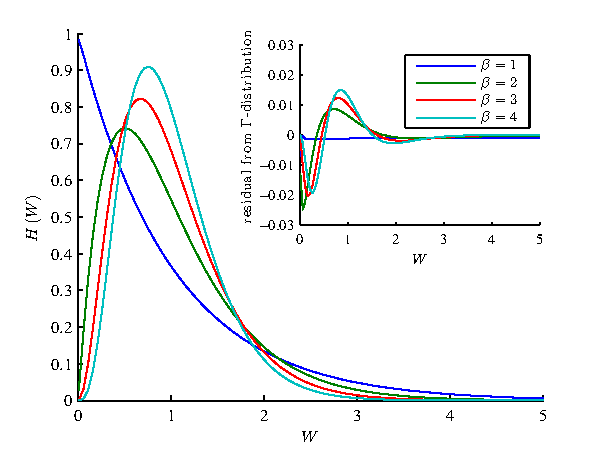
\includegraphics[width=0.5\textwidth]{/home/genneth/Documents/super-limit/gamma-set}
\par\end{centering}

\caption{\label{fig:g-gamma-limits}Limit distributions for binary fission
with $\Gamma$-distributed cell cycle lengths. Inset shows that the
limit distributions are very close $\Gamma$-distributions, but not
exactly.}
\end{figure}


Since the transform in equation \ref{eq:forwards-eq} is continuous,
the limit distribution will not change qualitatively for moderate
changes to the cell cycle distribution. In particular, the biologically
relevant example of a mono-modal distribution with an initial refractory
period is sufficiently close to give very similar limit distributions.
In any case, since the right tail is always exponential (appendix
\ref{app:moment-theorems}), the only qualitative change possible
is the behaviour near the origin, i.e. increase the proportion of
clones smaller than the average.

First, we may consider a process where the division of each cell can
produce a large number of progeny relative to the average. Specifically,
consider 
\[
f(s)=\sum_{k=0}^{\infty}\frac{s^{k}}{2^{k}}=\frac{s}{s-2}.
\]
 For the Markovian process it is possible \cite[III.8, theorem 3]{Athreya2004}
to analytically obtain the limit distribution 
\[
H(W)=\frac{1}{2}\left[-1+\frac{2e^{-W/4}}{\sqrt{\pi}\sqrt{W}}+\mathrm{erf}\left(\frac{\sqrt{W}}{2}\right)\right],
\]
which has a weak divergence at the origin. More intuitively, if we
consider the distribution of $\log W$, i.e. 
\begin{align*}
J(s)=H\left(e^{s}\right)e^{s} & =\frac{e^{\frac{s}{2}-\frac{e^{s}}{4}}}{\sqrt{\pi}}-\frac{1}{2}e^{s}\mathrm{erfc}\left(\frac{e^{s/2}}{2}\right)\\
 & \sim\frac{1}{\sqrt{\pi}}e^{s/2}\textrm{, }s\rightarrow-\infty,
\end{align*}
we see that it still decays exponentially.

Alternatively, we can simply have some cells which divide very slowly.
In particular, \figref{g-power-limits} shows the limit distributions
for binary fission with the family 
\begin{equation}
g(t)=\frac{\mathrm{sinc}\left(\frac{n}{\pi}\right)}{1+\left(t-\frac{1}{2}\right)^{n}}\Theta\left(t-\frac{1}{2}\right),\ n\ge2.\label{eq:power-law-g}
\end{equation}
As can be seen in the inset, the corresponding distribution in $\log W$
has a power-law tail for small $W$, implying a divergence 
\[
H(W)\approx\frac{C}{W\log^{n}W},\ W\rightarrow0.
\]
Notice however, that the local minimum in $H$ becomes closer to zero
as $n\rightarrow\infty$, and the divergence at the origin become
more narrow. If we impose an upper-end cut-off to $g(t)$, then the
divergence is removed, without significant changes to the rest of
the curve.

\begin{figure*}[t]
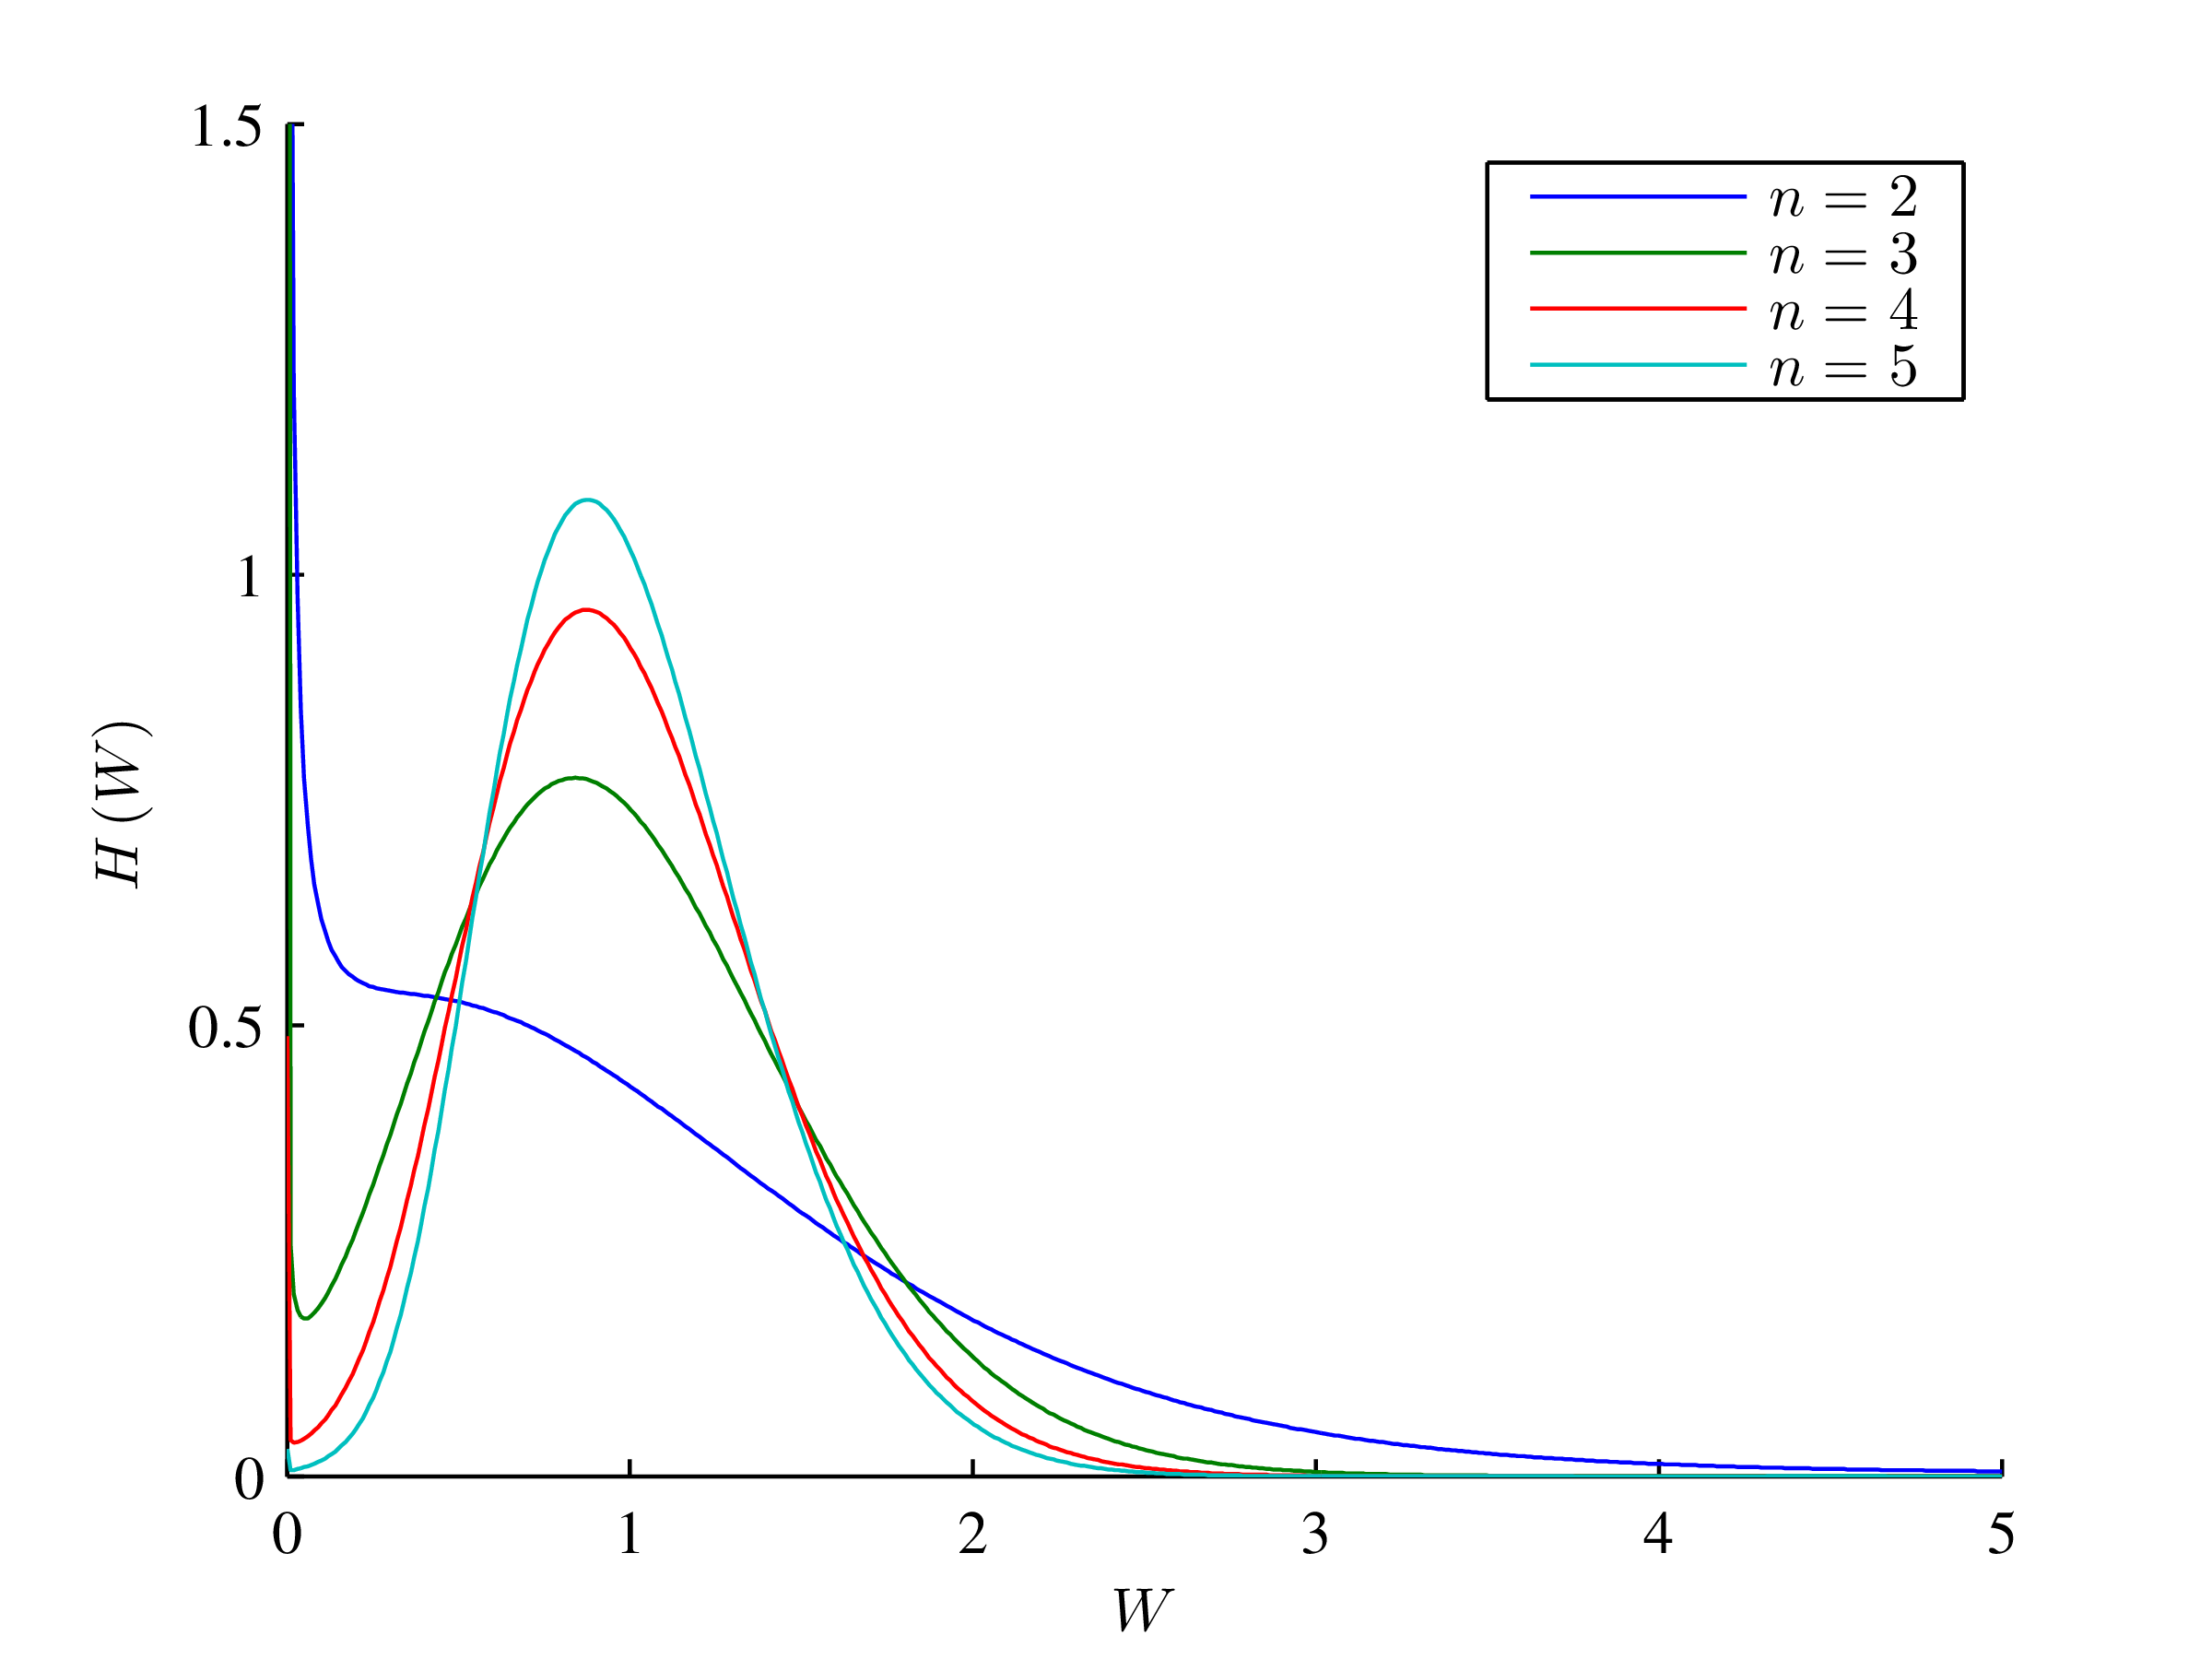
\includegraphics[width=0.5\textwidth]{/home/genneth/Documents/super-limit/power-set-W}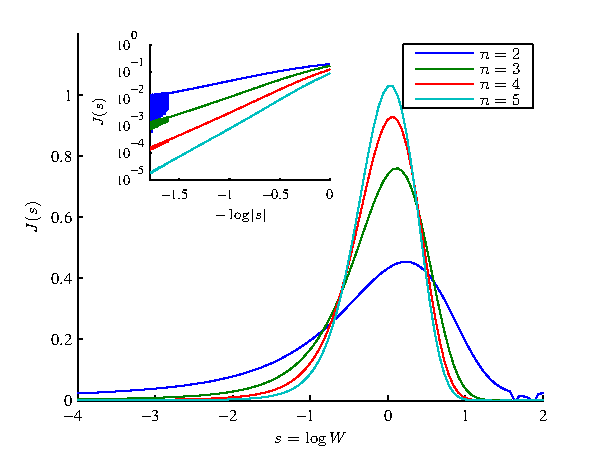
\includegraphics[width=0.5\columnwidth]{/home/genneth/Documents/super-limit/power-set-log-W}

\caption{\label{fig:g-power-limits}Limit distributions for binary fission
power-law tailed cell cycles. Left shows the divergence which occurs
at $W\rightarrow0$. Right shows the distribution of $\log W$, which
has power-law tails for large negative $\log W$ (inset). The very
right tail, and the left tail of the inset shows numerical noise;
the distributions are uniformly continuous.}
\end{figure*}



\section{\label{app:injective-continuity}Injectiveness and continuity of
\eqref{forwards-eq}}


\subsection*{Injectiveness}

Assume that two different $g_{1}$ and $g_{2}$ give the same $\phi$
upon transform with \eqref{forwards-eq}. We may assume without loss
of generality that their respective Malthusian parameters $\alpha$
are equal and unity (if they are not we can simply scale the cell
cycle distributions). Then we have
\[
\int_{0}^{\infty}f\left[\phi\left(e^{t-y}\right)\right]\left[g_{1}\left(y\right)-g_{2}\left(y\right)\right]dy=0,
\]
for all $t$. Using the convolution theorem we get 
\[
\widetilde{f\odot\phi}\left(\omega\right)\left[\tilde{g}_{1}\left(\omega\right)-\tilde{g}_{2}\left(\omega\right)\right]=0
\]
for $\Im\left\{ \omega\right\} >0$, obtaining that $\tilde{g}_{1}$
and $\tilde{g}_{2}$ are analytic, regular and equal on an open strip.
Thus as characteristic functions they are equal, and the original
functions $g_{1}$ and $g_{2}$ are equal as distributions.


\subsection*{Continuity}

Having established injectiveness, and since Fourier transforms are
continuous, it is sufficient to establish the continuity of \eqref{backward-eq}.
Letting $h(t)=h_{0}(t)+\delta h(t)$, we get $f\left[h(t)\right]=f\left[h_{0}(t)\right]+\delta h\left(t\right)f^{\prime}\left[h_{0}\left(t\right)\right]$.
Since $0\le h_{0}(t)\le1$, $f^{\prime}(s)$ is bounded within $0\le s\le1$
so define $A=\sup_{t}f^{\prime}\left[h_{0}\left(t\right)\right]$.
Taking norms of \eqref{backward-eq}, we can straightforwardly compute:
\begin{align*}
\left\Vert \widetilde{\delta g}\right\Vert  & =\frac{\left\Vert \tilde{h}_{0}\right\Vert +\left\Vert \widetilde{\delta h}\right\Vert }{\left\Vert \widetilde{f\odot h_{0}}\right\Vert +\left\Vert \widetilde{\delta h\, f^{\prime}\left[h_{0}\right]}\right\Vert }-\left\Vert \tilde{g}_{0}\right\Vert \\
 & =\left\Vert \widetilde{\delta h}\right\Vert \left\Vert \widetilde{f\odot h_{0}}\right\Vert -\left\Vert \tilde{h}_{0}\right\Vert \left\Vert \widetilde{\delta h\, f^{\prime}\left[h_{0}\right]}\right\Vert +O\left[\left\Vert \widetilde{\delta^{2}h}\right\Vert \right]\\
 & \le\left\Vert \widetilde{\delta h}\right\Vert \left\{ \left\Vert \widetilde{f\odot h_{0}}\right\Vert +A\left\Vert \tilde{h}_{0}\right\Vert \right\} +O\left[\left\Vert \widetilde{\delta^{2}h}\right\Vert \right].
\end{align*}



\section{\label{app:moment-theorems}Of moments and tails}

Differentiating equation \ref{eq:forwards-eq} we get (via Fa\`a
di Bruno's formula):

\[
\phi^{(n)}(u)=\int_{0}^{\infty}\left\{ \sum_{\mathbf{k}}\frac{n!}{k_{1}!\cdots k_{n}!}f^{(k)}\left[\phi\left(ue^{-y}\right)\right]\left[\frac{\phi^{(1)}\left(ue^{-y}\right)e^{-y}}{1!}\right]^{k_{1}}\cdots\left[\frac{\phi^{(n)}\left(ue^{-y}\right)e^{-ny}}{n!}\right]^{k_{n}}\right\} g(y)\, dy
\]
where the summation runs over all partitions of $n$ such that $k_{1}+2k_{2}+\cdots+nk_{n}=n$
and $k=k_{1}+\cdots+k_{n}$. Recognising these as moments (up to factors
of $i$ which may be removed without loss of generality by picking
the right boundary conditions for $\phi$) gives (using the fact that
$M_{0}=\phi(0)=1$): 
\begin{equation}
M_{n}=\sum_{\mathbf{k}}\frac{n!}{k_{1}!\cdots k_{n}!}f^{(k)}\left(1\right)\left(\frac{M_{1}}{1!}\right)^{k_{1}}\cdots\left(\frac{M_{n}}{n!}\right)^{k_{n}}\int_{0}^{\infty}e^{-ny}g(y)\, dy.\label{eq:moment-recursion}
\end{equation}


Since we assumed that all moments of $f$ exist, $f^{(k)}(1)$ will
also exist. Noticing that there is only one partition with $k_{n}=1$,
we can move that term to the left hand side and we get for $n\ge2$
\[
M_{n}\left[1-\int_{0}^{\infty}f^{\prime}(1)e^{-ny}g(y)\, dy\right]=C\left[M_{1},\ldots,M_{n-1}\right],
\]
where the right hand side only depends on the lower moments, and in
particular is finite if all the lower moments are finite. Then
\[
1=\int_{0}^{\infty}f^{\prime}(1)e^{-y}g(y)\, dy>\int_{0}^{\infty}f^{\prime}(1)e^{-ny}g(y)\, dy
\]
and since $M_{1}=1$ is finite, by induction all moments exist. Thus,
applying Chebychev's inequality we get $H(W)\in o\left(W^{-\alpha}\right)$
for all $\alpha$. We conjecture that it is actually exponentially
bounded, and show this below for binary fission.

We now outline an argument that the tails are also bounded from below
by an exponential. First, generally if two non-negative variables
$W_{1}$ and $W_{2}$ have moments obeying
\[
\mathbb{E}\left[W_{1}^{n}\right]\ge\mathbb{E}\left[W_{2}^{n}\right]
\]
 for all $n$, then there exists a $w_{0}$ such that for all $w>w_{0}$
\[
\mathbb{P}\left[W_{1}>w\right]\ge\mathbb{P}\left[W_{2}>w\right].
\]
To see this, consider the contrapositive, which is that if the set
of $w$ where $\mathbb{P}\left[W_{1}>w\right]<\mathbb{P}\left[W_{2}>w\right]$
is unbounded, then for at least one $n$, $\mathbb{E}\left[W_{1}^{n}\right]<\mathbb{E}\left[W_{2}^{n}\right]$.
We then check two cases: (a) if it there exist arbitrarily large $w$
such that $\mathbb{P}\left[W_{1}>w\right]>\mathbb{P}\left[W_{2}>w\right]$
then it would be a contradiction for the moments to be dominated 

Second, if the moments $\log\mathbb{E}\left[W^{n}\right]\in n\log n+\Theta(n)$
for large $n$ then the tail $\mathbb{P}\left[W>w\right]$ is exponential,
in some sense. In particular, existing work \cite{Abate1996} suggests
that if the limits 
\[
\eta_{n}=\frac{n\mathbb{E}\left[W^{n-1}\right]}{\mathbb{E}\left[W^{n}\right]}\rightarrow\eta
\]
 and 
\[
A_{n}=\frac{\eta_{n}^{n}\mathbb{E}\left[W^{n}\right]}{n!}\rightarrow A
\]
 exist, then 
\[
\lim_{w\rightarrow\infty}e^{\eta w}\mathbb{P}\left[W>w\right]=A.
\]
 Finally, we consider equation \ref{eq:moment-recursion} and drop
all terms higher than quadratic

\begin{equation}
\frac{M_{n}}{n!}\ge\sum_{k=1}^{n-1}\frac{M_{k}M_{n-k}}{k!(n-k)!}\frac{f^{\prime\prime}(1)\int_{0}^{\infty}e^{-ny}g(y)\, dy}{1-f^{\prime}(1)\int_{0}^{\infty}e^{-ny}g(y)\, dy}\label{eq:moments-lower-bound}
\end{equation}
which follows as each term in equation \ref{eq:moment-recursion}
is positive. Defining $\xi(n)=M_{n}/n!$ we have
\[
\xi(n)\ge\sum_{k=1}^{n-1}\xi(k)\xi(n-k)K_{n},
\]
where 
\begin{align*}
K_{n} & =\frac{f^{\prime\prime}(1)\int_{0}^{\infty}e^{-ny}g(y)\, dy}{1-f^{\prime}(1)\int_{0}^{\infty}e^{-ny}g(y)\, dy}\\
 & >\frac{f^{\prime\prime}(1)}{1-f^{\prime}(1)\int_{0}^{\infty}e^{-2y}g(y)\, dy}\int_{0}^{\infty}e^{-ny}g(y)\, dy\\
 & \ge C\eta^{-n}
\end{align*}
for some $C$ and $\eta$. Using the equality we can convert this
into a lower bound 
\[
M_{n}\ge\frac{n!}{C\eta^{n}}
\]
which by the above gives an exponential tail. Thus, we conclude that
the tail of a limit distribution is exponentially bounded.

In the case of binary fission, we can improve the upper bound slightly.
In particular, the equality in \eqref{moments-lower-bound} applies.
An upper bound on the moments is then given by
\[
\frac{K_{2}M_{n}}{n!}\le\sum_{k=1}^{n-1}\frac{K_{2}M_{k}}{k!}\frac{K_{2}M_{n-k}}{(n-k)!}.
\]
with equality for $n\le2$, where 
\[
K_{2}=\frac{2\int_{0}^{\infty}e^{-2y}g(y)\, dy}{1-2\int_{0}^{\infty}e^{-2y}g(y)\, dy}.
\]
We obtain an upper bound in terms of the Catalan numbers
\[
\frac{K_{2}M_{n}}{n!}\le\frac{K_{2}^{n}(2n-2)!}{(n-1)!n!}
\]
Then applying the moments bound\cite{Philips1995} we have
\[
\mathbb{P}\left[W>w\right]=\inf_{n}\frac{M_{n}}{w^{n}}\le\inf_{n}\frac{K_{2}^{n-1}(2n-2)!}{(n-1)!w^{n}},
\]
which for large $w$ gives 
\[
\mathbb{P}\left[W>w\right]=O\left(\frac{1}{w}\right)e^{-\frac{w}{4K_{2}}}.
\]


Finally, we note that removing the assumption that all moments of
$f$ exist will remove the upper bound but not the exponential lower
bound. Furthermore, if the $k$'th moment of $f$ is infinite, then
the $k$'th moment of $H$ will be as well, suggesting a tail $H(W)\approx W^{-k-1}$;
indeed, the moment will diverge at finite times.


\section{\label{app:examples}Applications of the Klein inversion formula}


\subsection*{Delta distribution}

If $H(W)=\delta(W-1)$ then $\phi(u)=e^{iu}$ and $h(t)=e^{ie^{t}}$,
thus $\tilde{h}(\omega)=e^{\pi\omega/2}\Gamma\left(-i\omega\right)$,
defined for $0<\Im(\omega)<1$. For 
\[
f(s)=\sum_{k=1}^{\infty}p_{k}s^{k}
\]
 (notice that we do not have a constant term), 
\[
\widetilde{f\odot h}(\omega)=e^{\pi\omega/2}\Gamma\left(-i\omega\right)\sum_{k=1}^{\infty}p_{k}k^{i\omega}
\]
defined on the same strip. The quotient is then well defined:
\[
\tilde{g}(\omega)=\frac{1}{\sum_{k=1}^{\infty}p_{k}k^{i\omega}}.
\]
If only one $p_{k}$ is non-zero (and therefore equal to one), we
would have a well-defined distribution
\[
g(t)=\delta(t-\ln k),
\]
which reproduces the trivial result that a discrete time Markovian
process with fixed outcomes in each division necessarily leads to
a Dirac distribution as the limit. For a more generic $f$ it does
not lead to a probability distribution.


\subsection*{Exponential tailed distributions}

As conjectured, the tail of $H$ is always exponential. With the integral
above we can consider the very general class
\[
H(W)=\sum_{k}a_{k}\frac{\lambda^{k+1}}{\Gamma(k+1)}W^{k}e^{-\lambda W}
\]
where normalisation requires $\sum_{k}a_{k}=1$ and unity mean requires
$\sum_{k}a_{k}(k+1)/\lambda=1$, though as we shall see the latter
will be automatically enforced. The characteristic function is very
helpfully just a sum
\[
\phi(u)=\sum_{k}a_{k}\left(1-\frac{iu}{\lambda}\right)^{-k-1}.
\]
Importantly, $f\odot\phi$ has the same structure, composed of a linear
combination of $(1-iu/\lambda)^{-n}$. Thus we only have to consider
a single integral (convergent on $-k-1<\Im\{\omega\}<0$):

\begin{align*}
 & \int_{-\infty}^{\infty}e^{i\omega t}\left(1-\frac{ie^{t}}{\lambda}\right)^{-k-1}dt\\
= & \lambda^{i\omega}\int_{0}^{\infty}z^{i\omega-1}(1-iz)^{-k-1}dz\\
= & \lambda^{i\omega}e^{-\pi\omega/2}\frac{\Gamma\left(1+k-i\omega\right)\Gamma\left(i\omega\right)}{\Gamma(1+k)}\\
= & \lambda^{i\omega}e^{-\pi\omega/2}\Gamma(1-i\omega)\Gamma\left(i\omega\right)\frac{\left(1-i\omega\right)_{k}}{\Gamma(1+k)}
\end{align*}
where $\left(z\right)_{n}$ is the Pochhammer symbol. In \eqref{backward-eq},
upon taking the quotient all but the last factor above cancel. Define
the auxiliary polynomials $P(z)=\sum_{k}a_{k}z^{k}$ and $Q(z)=\frac{1}{z}f\left[zP(z)\right]$
and a transform on polynomials defined by being linear and acts on
each monomial as 
\[
\widehat{z^{k}}\Longrightarrow\frac{(1+z)_{k}}{\Gamma(k+1)}.
\]
Then by linearity we immediately get
\[
\tilde{g}(\omega)=\frac{\widehat{P}(-i\omega)}{\widehat{Q}(-i\omega)}.
\]
Notice that the formula above is completely independent of $\lambda$;
the correct one such that $H(W)$ has mean of unity will be chose.
We can find $g(t)$ by applying the Heaviside formula to $\tilde{g}(iz)$
(treating it as an inverse Laplace transform), and generically it
will be a sum of exponentials (possibly with complex exponents, but
always occurring in conjugate pairs), determined by the locations
of zeros of $\hat{Q}$. Note that whilst $\hat{Q}(z)$ cannot have
any zeros on the positive real line, generically there may be zeros
on the right half plane. Below, we will try and give some simple cases
where this can be done and it yields proper cell cycle distributions.

The simplest case is $H(W)=e^{-W}$ which corresponds to $\lambda=1$,
$P(z)=1$ and $Q(z)=\frac{1}{z}f(z)$. Thus,
\[
\tilde{g}(\omega)=\frac{1}{\sum_{k}p_{k}(1-i\omega)_{k-1}/\Gamma(k)}.
\]
If only one $p_{k}$ is non-zero, then
\[
g(t)=(k-1)e^{-(k-1)t}\left(e^{t}-1\right)^{k-2}.
\]
In particular this reproduces the result that for binary fission ($k=2$)
the Markovian process ($g(t)=e^{-t}$) gives an exponential distribution
in the limit. Biologically cells can only divide into two, so we can
consider $f(z)=(1-r)z+rz^{2}.$ In that case, 
\[
g(t)=\frac{1}{r}e^{-t/r},
\]
 which is again Markovian, and, in hindsight obvious.

Another simple case is when $H$ is a $\Gamma$-distribution; in that
case, $\lambda=\beta$, $P(z)=z^{\beta-1}$ and $Q(z)=\frac{1}{z}f\left(\beta^{\beta}z^{\beta}\right)$.
We get
\begin{align*}
\tilde{g}(\omega) & =\frac{(1-i\omega)_{\beta-1}/\Gamma(\beta)}{\sum_{k}p_{k}(1-i\omega)_{k\beta-1}/\Gamma(k\beta)}\\
 & =\left[\sum_{k}p_{k}\frac{(\beta-i\omega)_{(k-1)\beta}}{(\beta)_{(k-1)\beta}}\right]^{-1}.
\end{align*}
If only one $p_{k}$ is non-zero then the poles are simple and line
on the positive imaginary axis, and furthermore $g(t)$ is positive:
\[
g(t)=\frac{\Gamma(k\beta)}{\Gamma(\beta)\Gamma\left[(k-1)\beta\right]}e^{-(k\beta-1)t}\left(e^{t}-1\right)^{(k-1)\beta-1}.
\]
Note that this reproduces, in appropriate limits, the results above
for $H(W)=e^{-W}$ and $H(W)=\delta(W-1)$. Figure \ref{fig:H-gamma}
shows some examples from this family.

\begin{figure}[t]
\begin{centering}
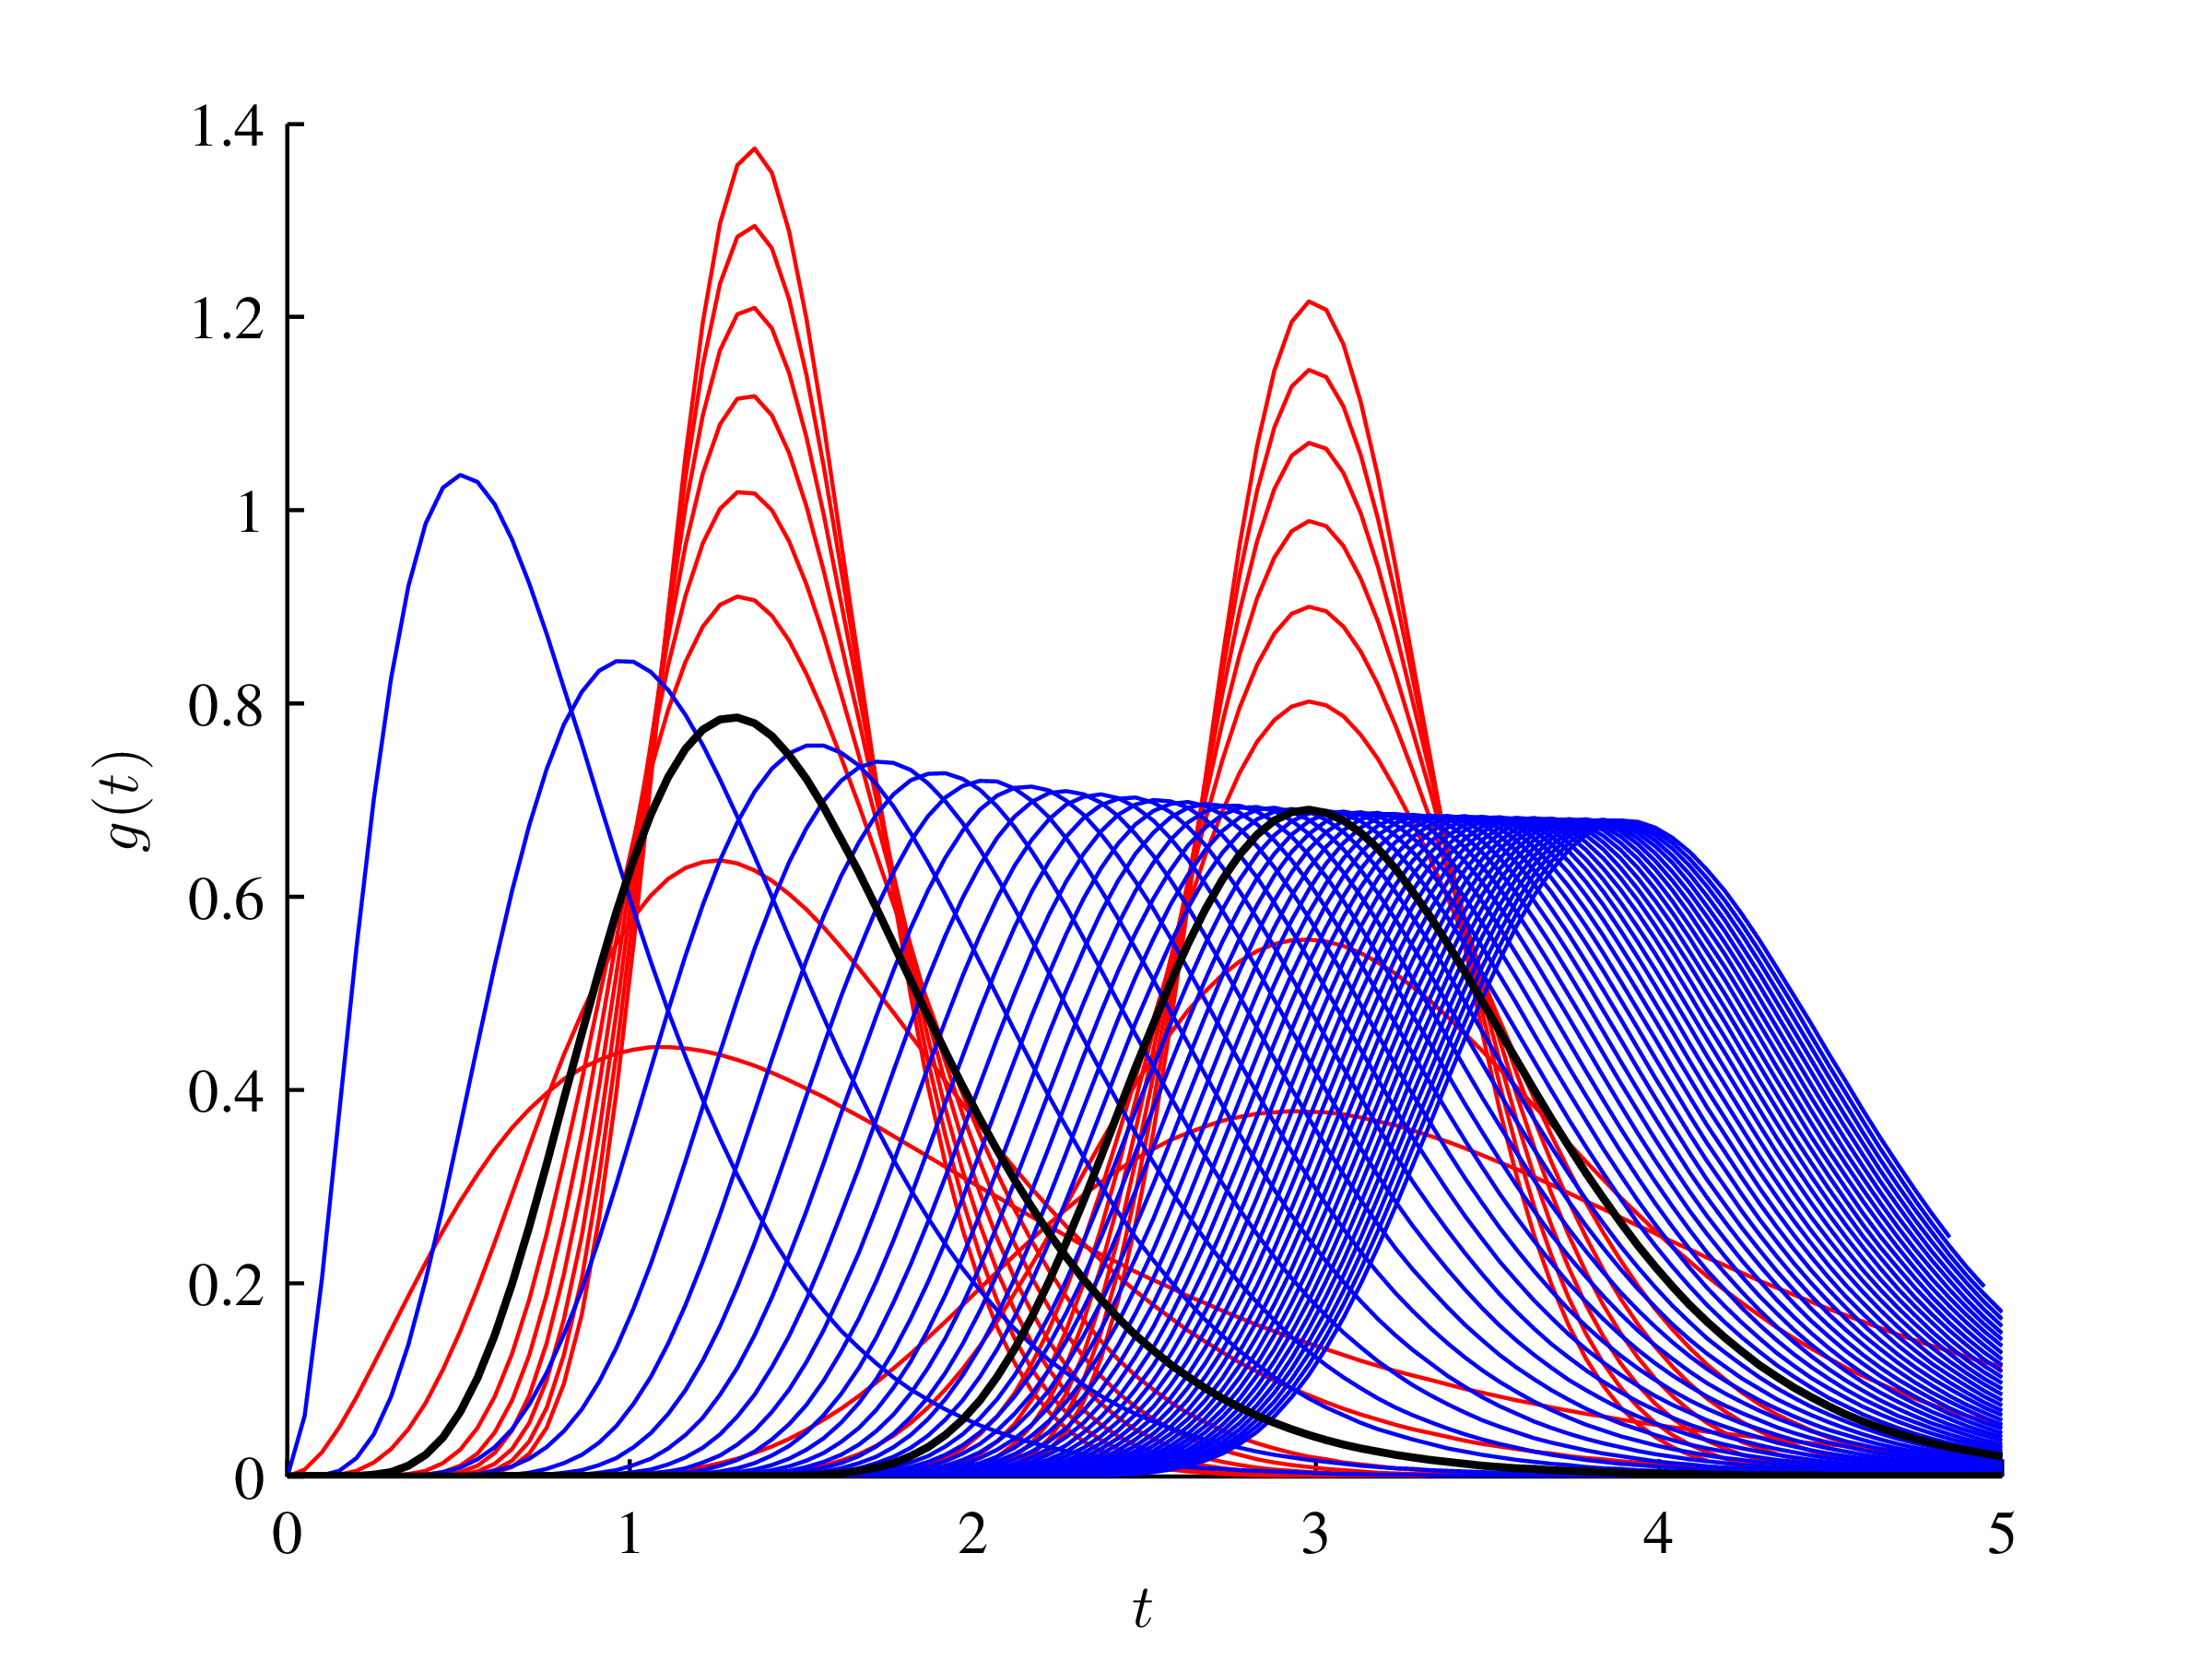
\includegraphics[width=0.5\textwidth]{/home/genneth/Documents/super-limit/gamma-inverse}
\par\end{centering}

\caption{\label{fig:H-gamma}Cell cycle distributions that gives $\Gamma$-distributions
with shape parameter $\beta$ as limit distributions, when each cell
divides exactly into $k$ at the end of its life. In blue we show
the variation as $k=2,3,\ldots,50$ for fixed $\beta=3$. The two
red series show variation of $\beta=1,\ldots,9$ for $k=4$ and $k=20$.
In thick black, we show the intersections $k=4,\ \beta=3$ and $k=20,\ \beta=3$.
As $k\rightarrow\infty$ the distributions approach a Dirac delta
distribution, with mean $\ln k$.}
\end{figure}


We note that the above is well-defined for all positive real $\beta$,
not only positive integers. In addition, for $k=2$, it produces a
family of distributions which when scaled to have unit mean is well-approximated
by the $\Gamma$-distributions $\beta^{\beta}e^{-\beta t}t^{\beta-1}/\Gamma(\beta)$.
Lastly, for $\beta=1/(k-1)$, we get an exponential distribution for
$g$, thus solving the Markovian problem for branching with a single
$k$.

More generically, it becomes very difficult to find the conditions
such that the Klein formula is well-defined. Consider even the restricted
case that $f(z)=(1-r)z+rz^{2}$, i.e. a generic biologically sensible
branching process, starting with a $\Gamma$-distribution:
\[
\tilde{g}\left(\omega\right)=\left[(1-r)+r\frac{\left(\beta-i\omega\right)_{\beta}}{\left(\beta\right)_{\beta}}\right]^{-1}.
\]
Starting with $\beta=2$, we find 
\[
g(t)=\frac{6e^{-\frac{1}{2}\left(5+\sqrt{25-\frac{24}{r}}\right)t}\left(-1+e^{\sqrt{25-\frac{24}{r}}t}\right)}{\sqrt{r(-24+25r)}}
\]
which is only positive everywhere if $r>24/25$, in which case all
exponents are real. However, for $\beta=3$ 
\[
g(t)=\frac{60\left[\omega_{1}\left(e^{t\omega_{2}}-e^{t\omega_{3}}\right)+\omega_{2}\left(e^{t\omega_{3}}-e^{t\omega_{1}}\right)+\omega_{3}\left(e^{t\omega_{1}}-e^{t\omega_{2}}\right)\right]}{r\left(\omega_{1}-\omega_{2}\right)\left(\omega_{2}-\omega_{3}\right)\left(\omega_{3}-\omega_{1}\right)}
\]
where $\omega_{1,2,3}$ are the three roots to the cubic $60+47rz+12rz^{2}+rz^{3}=0$.
All three roots have negative real parts for $r\gtrsim0.106383$ but
$g(t)$ is not positive for most of that. Indeed, only for $r>\frac{90\left(270-\sqrt{3}\right)}{24299}\approx0.993626$
are all three roots real. Numerically, it seems that only if all three
roots are real is $g(t)$ well-defined. By similar arguments, for
$\beta=4$ we find that $r>\frac{840}{841}$; and for $\beta=5$,
$r\gtrsim0.999906$.

The example above required that the poles of $\tilde{g}$ lay only
on the imaginary axis, but this is not necessary. Consider binary
fission, $f(z)=z^{2}$, and a multi-modal $P(z)=r+(1-r)z^{3}$. The
denominator $Q(z)$ is of order 7. The roots are all real for $r\apprle9.164\times10^{-4}$
and five real roots for $r\apprle0.07036$. However, as \figref{multi-modal}
shows, there exist well-behaved solutions for $r\apprle0.35$, which
can be interestingly multi-modal. 

\begin{figure}
\begin{centering}
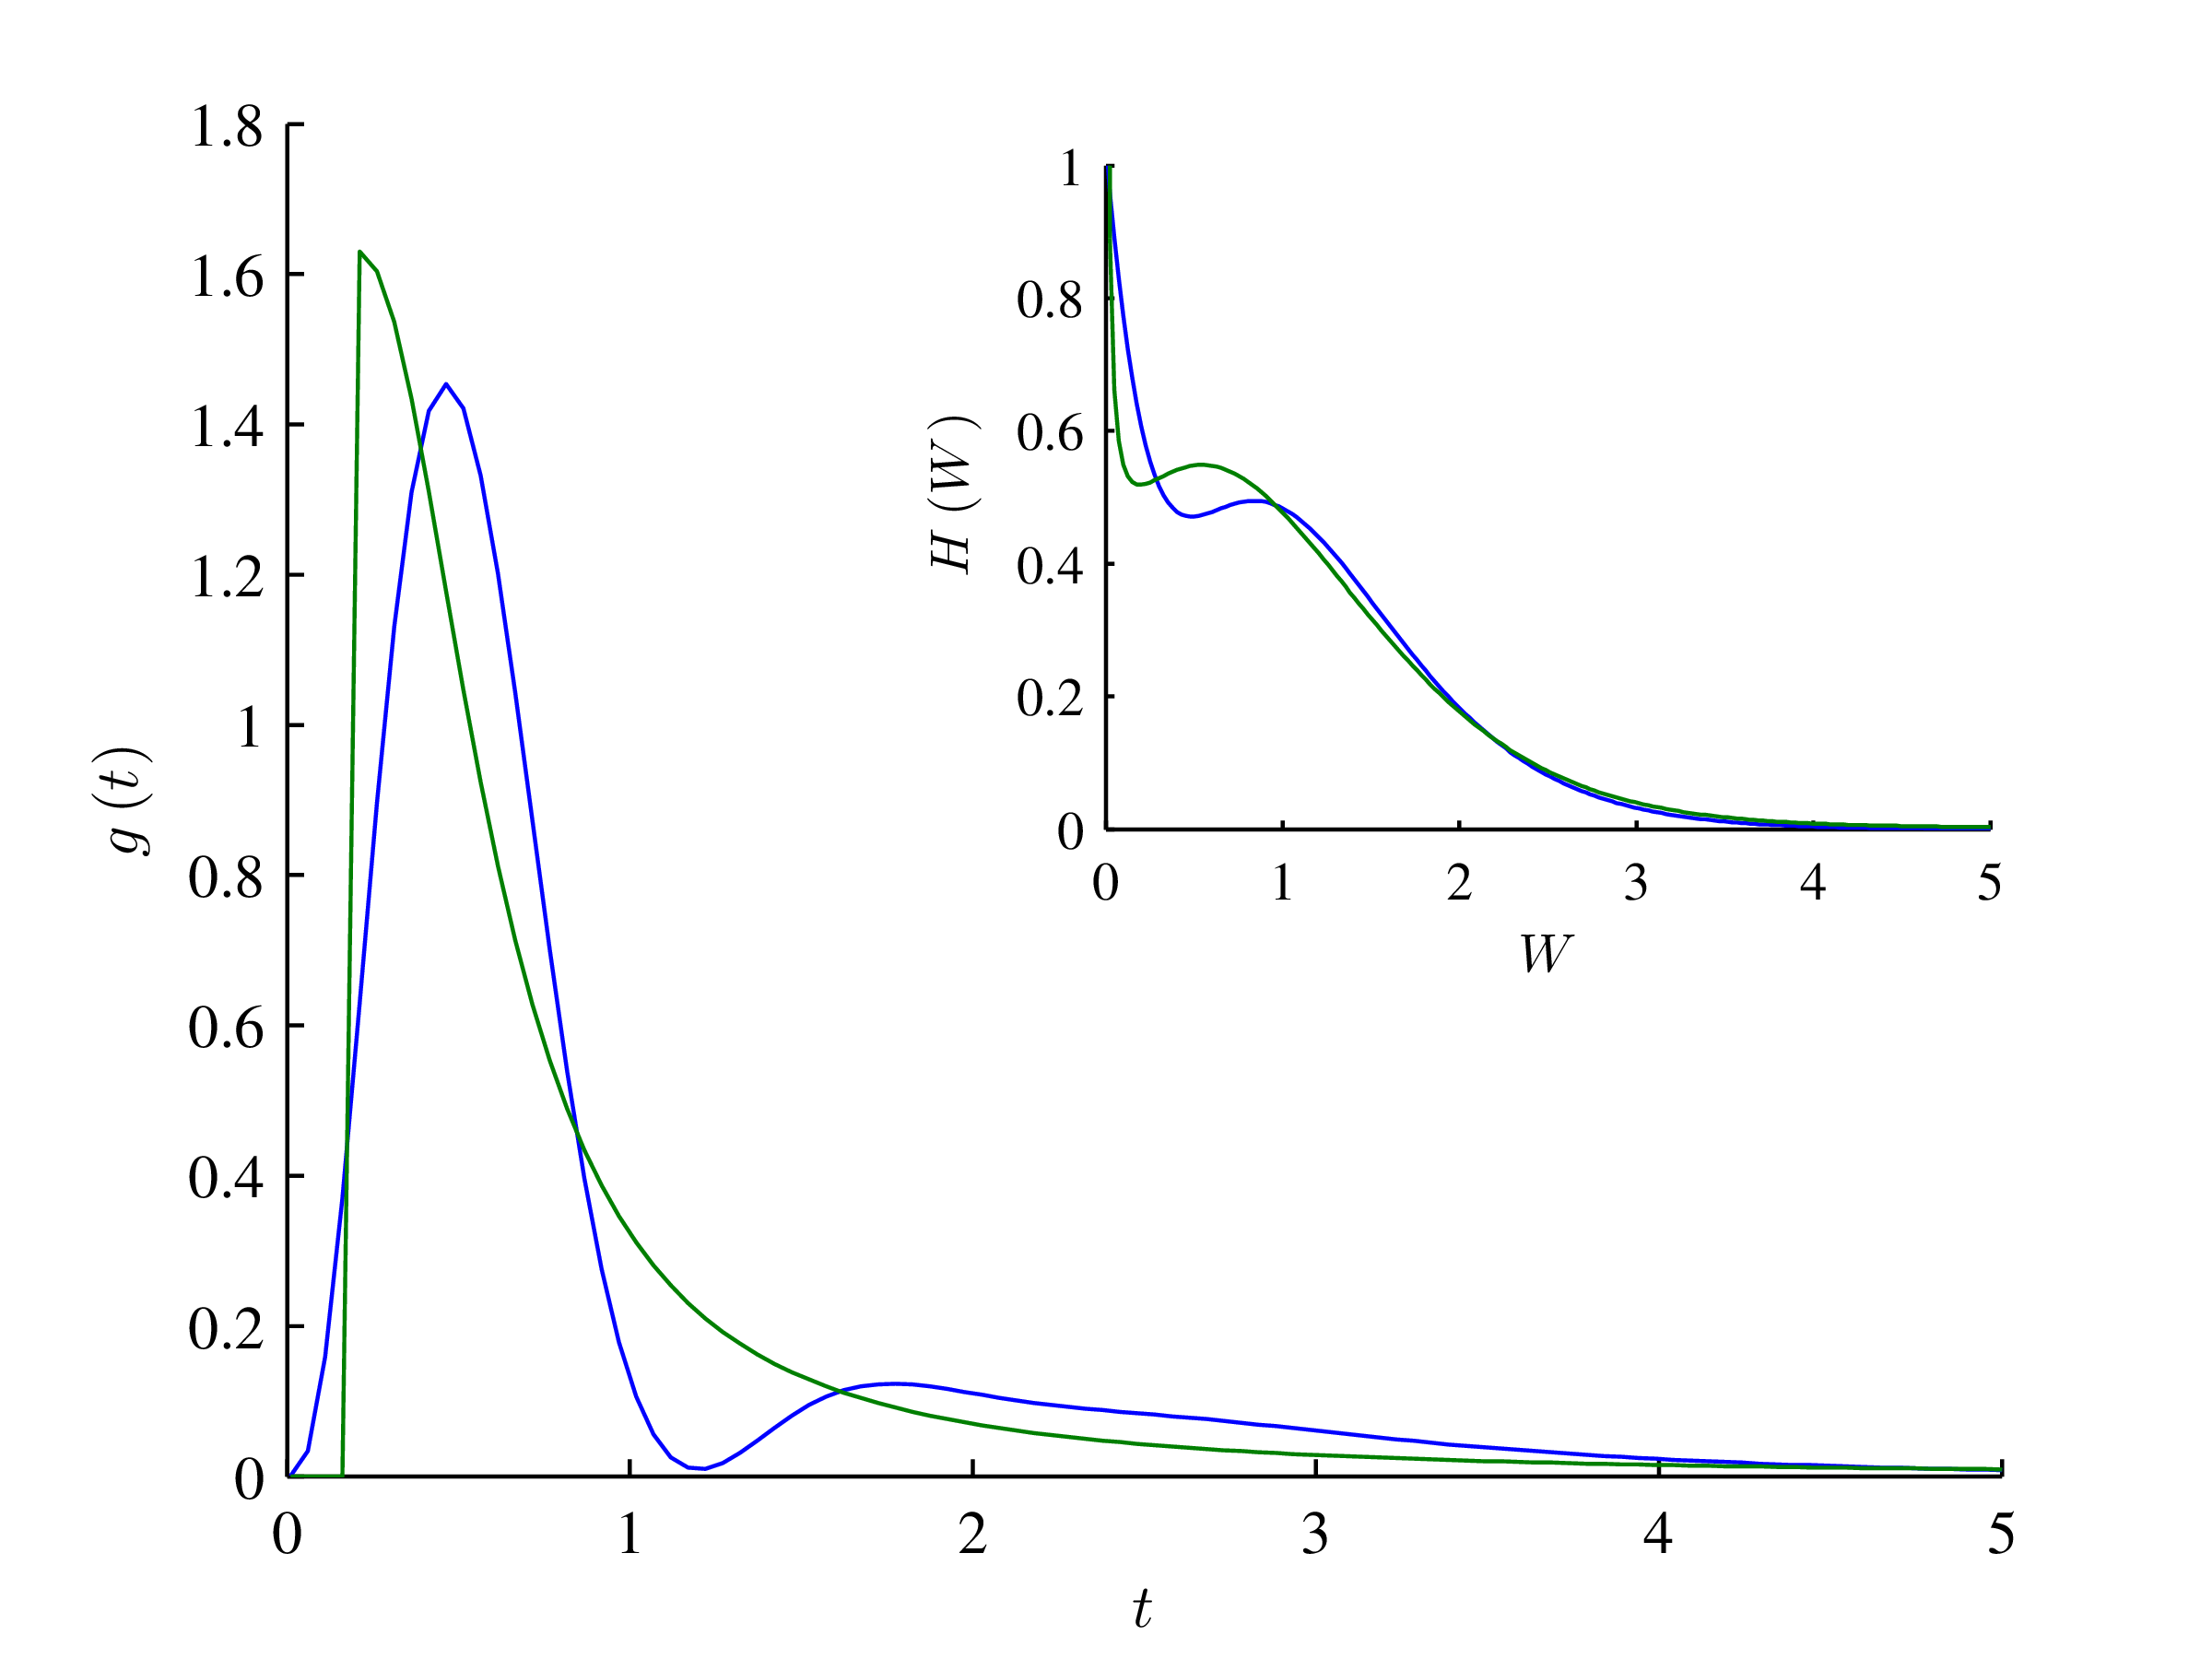
\includegraphics[width=0.5\textwidth]{/home/genneth/Documents/super-limit/multi-modal}
\par\end{centering}

\caption{\label{fig:multi-modal}Main figure shows the cell cycle distribution
which gives the limit distribution in the inset. Blue is for $H(W)=\left[r+(1-r)z^{3}W^{3}\lambda^{4}/\Gamma(4)\right]e^{-\lambda W}$
where $\lambda$ is such that $\int W\, H(W)\, dW=1$ and $r=0.35$.
Green is a comparison with the power-law tailed distribution from
\eqref{power-law-g} with $n=2.1$. For $r\apprge0.35$ the dip in
$g(t)$ becomes pronounced enough that it become negative. For $r\rightarrow0$
the distribution $g(t)$ is well-defined, but for $r\rightarrow1$
it is not, even though $r=1$ it is well-defined.}
\end{figure}



\chapter{Stochastic Fate Choice in Cultured Rat Retinal Progenitors}


\section{Chapter Overview}

The central question of developmental biology is how do cells organise
their divisions to achieve the same body plan reproducibly. One could
imagine that each cell is pre-programmed with the instructions (and
classical lineage tracing experiments in \emph{C. elegans} suggests
that this does occur {[}cite{]}), or alternatively there is some complex
emergent organisation which only manifests within the right environment
(?? shows the importance of cell-cell interactions for spermatogenesis).
Here we study rat retinal progenitors from day 20 \emph{in vitro};
these cells are late in the developmental process, and nearing complete
diffenentiation. Earlier work {[}Cayouette{]} had established that
even under culture conditions retinal progenitors cells (RPCs) will
generate the correct proportions of retinal cell types, even while
each individual RPC generates a heterogeneous collection of cells;
this raises the possibility that there is indeed a great deal of intrinsic
pre-programming, but expressed as a stochastic procedure which averages
over a population to give the correct outcome.

In this chapter, we focus on an experiment which tracks by time-lapse
microscopy cultured RPCs, from which detailed lineage trees may be
reconstructed, showing the exact time of divisions and fate outcomes.
We show that even though the pattern of divisions seem very complex,
there is a simple stochastic model which is consistent with the data.
This draws heavily on the work in {[}cite{]}; experimental work was
carried out by FLAFG, manuscript was written by MC, analysis by GZ
and BDS, with discussions with WAH, FC and JAC. In what follows we
will elide the exact experimental procedures, and refer the reader
to the published work {[}cite{]}.


\section{Experimental results}

To study retinal lineages, we cultured E20 rat RPCs at clonal density
and recorded their development over time using long-term time-lapse
microscopy. Over a period of more than 2 years, we followed the fate
of 2347 RPCs. Of these, 856 were excluded from further analysis because
the RPC either died (6.3\%), moved away from the field of view (2.7\%),
touched another cell that was not part of the clone (6.5\%), or immediately
differentiated without dividing (21\%). As a result, we recovered
a total of 1491 RPCs that divided at least once to generate clones
containing two cells or more.

From the 1491 RPCs, 1211 were recorded to have undergone a terminal
division that generated two differentiating daughters, but were not
further analyzed in terms of cell type composition. Of the remaining
280 RPCs that divided more than once, the lineage trees of 129 could
be reconstructed (all reconstructed lineages leading to clones of
three or more cells are shown in \figref{rat-raw}), whereas the remaining
clones had cells that were lost during the fixation and immunostaining
process, or the outcome of at least one mitosis could not be resolved,
most often owing to cells moving on top of each other.

In the successfully reconstructed lineages, there were 465 differentiated
cells, three of which had an unidentified fate (0.6\%), and in the
remaining cells we found 341 RPh (73.8\%), 59 Bi (12.8\%), 49 Am (10.6\%)
and 13 Mu (2.8\%). These proportions are similar to those obtained
after labeling RPCs at postnatal day (P) 0 with retroviral vectors
in the mouse retina (Turner et al., 1990).

We note that the reconstructed lineages vary widely in size and composition,
and there is no clear order in which cell types are generated. In
particular, almost all orderings of cell types occur, suggesting that
the order of retinal cell type production is not strictly encoded
in each lineage, at least not from E20 onwards in culture.

\begin{figure}
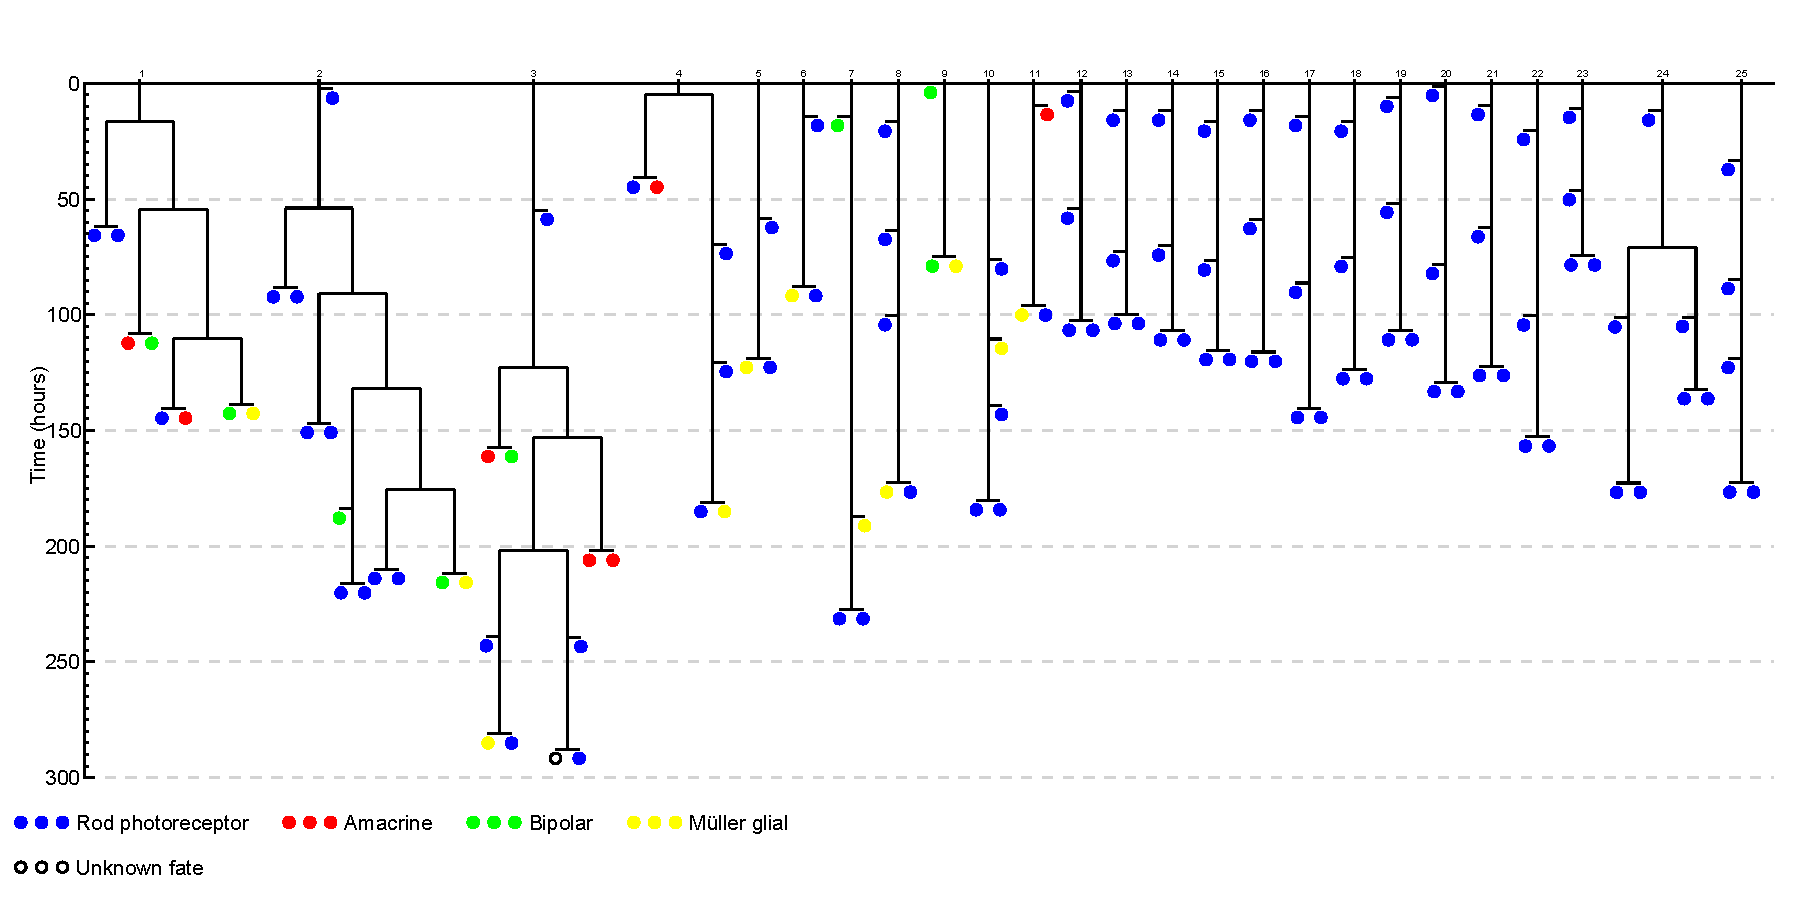
\includegraphics[width=0.5\columnwidth]{retinalLineageData1}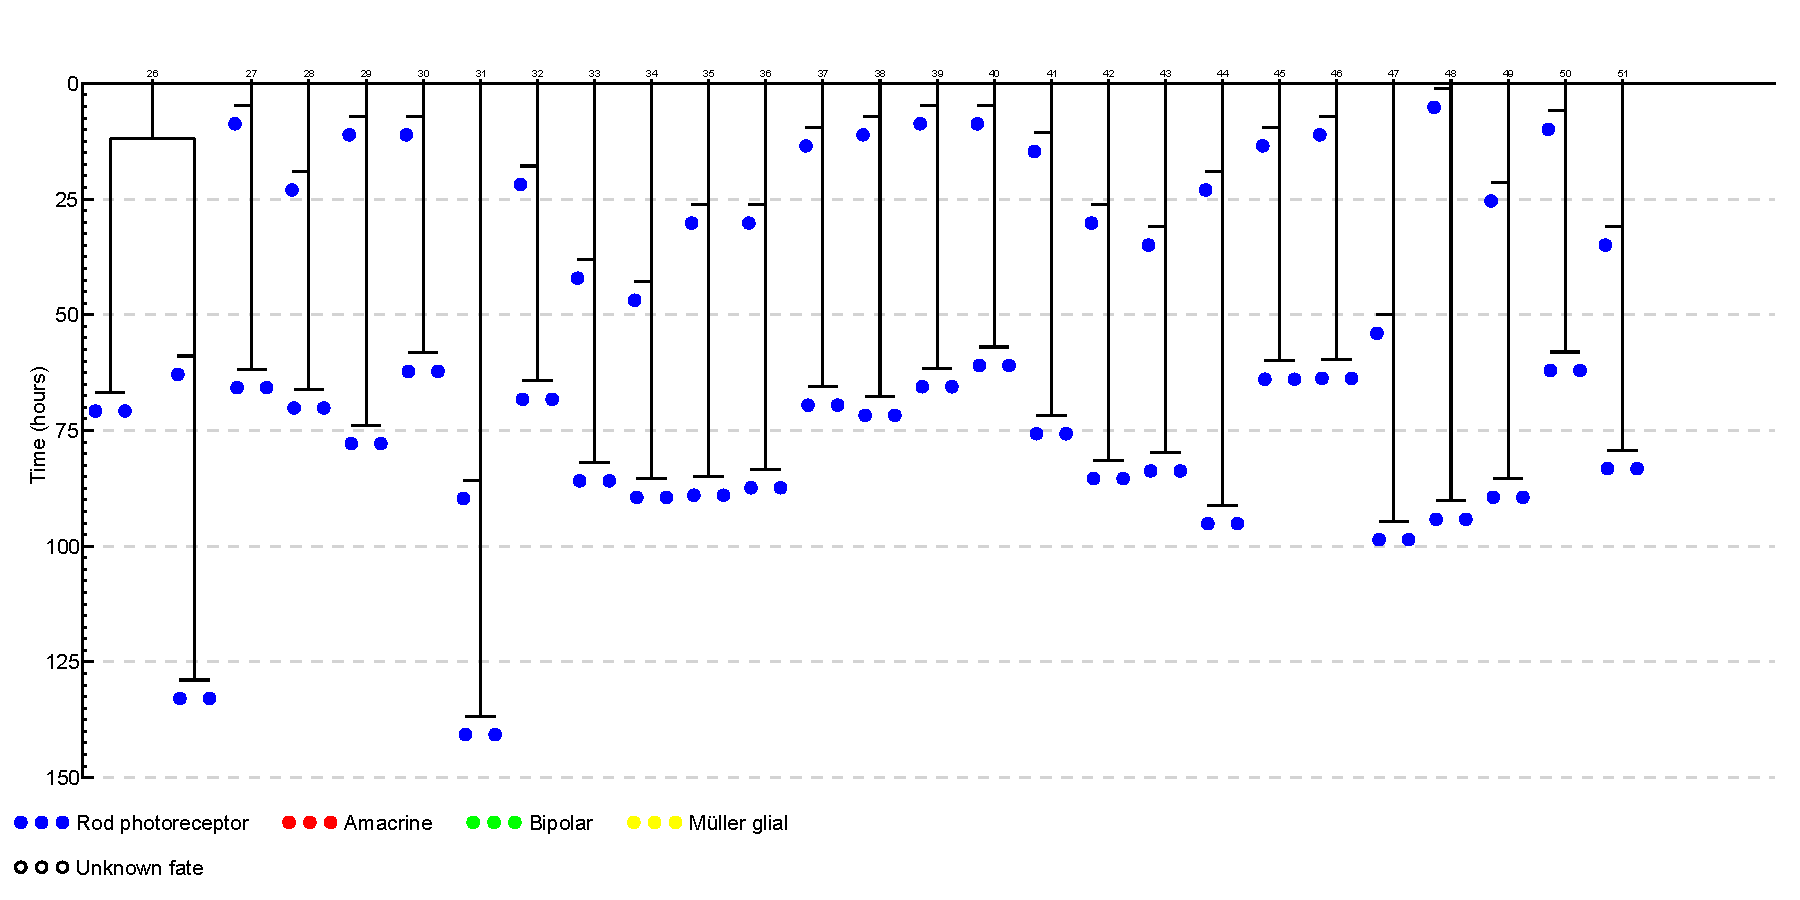
\includegraphics[width=0.5\columnwidth]{retinalLineageData2}

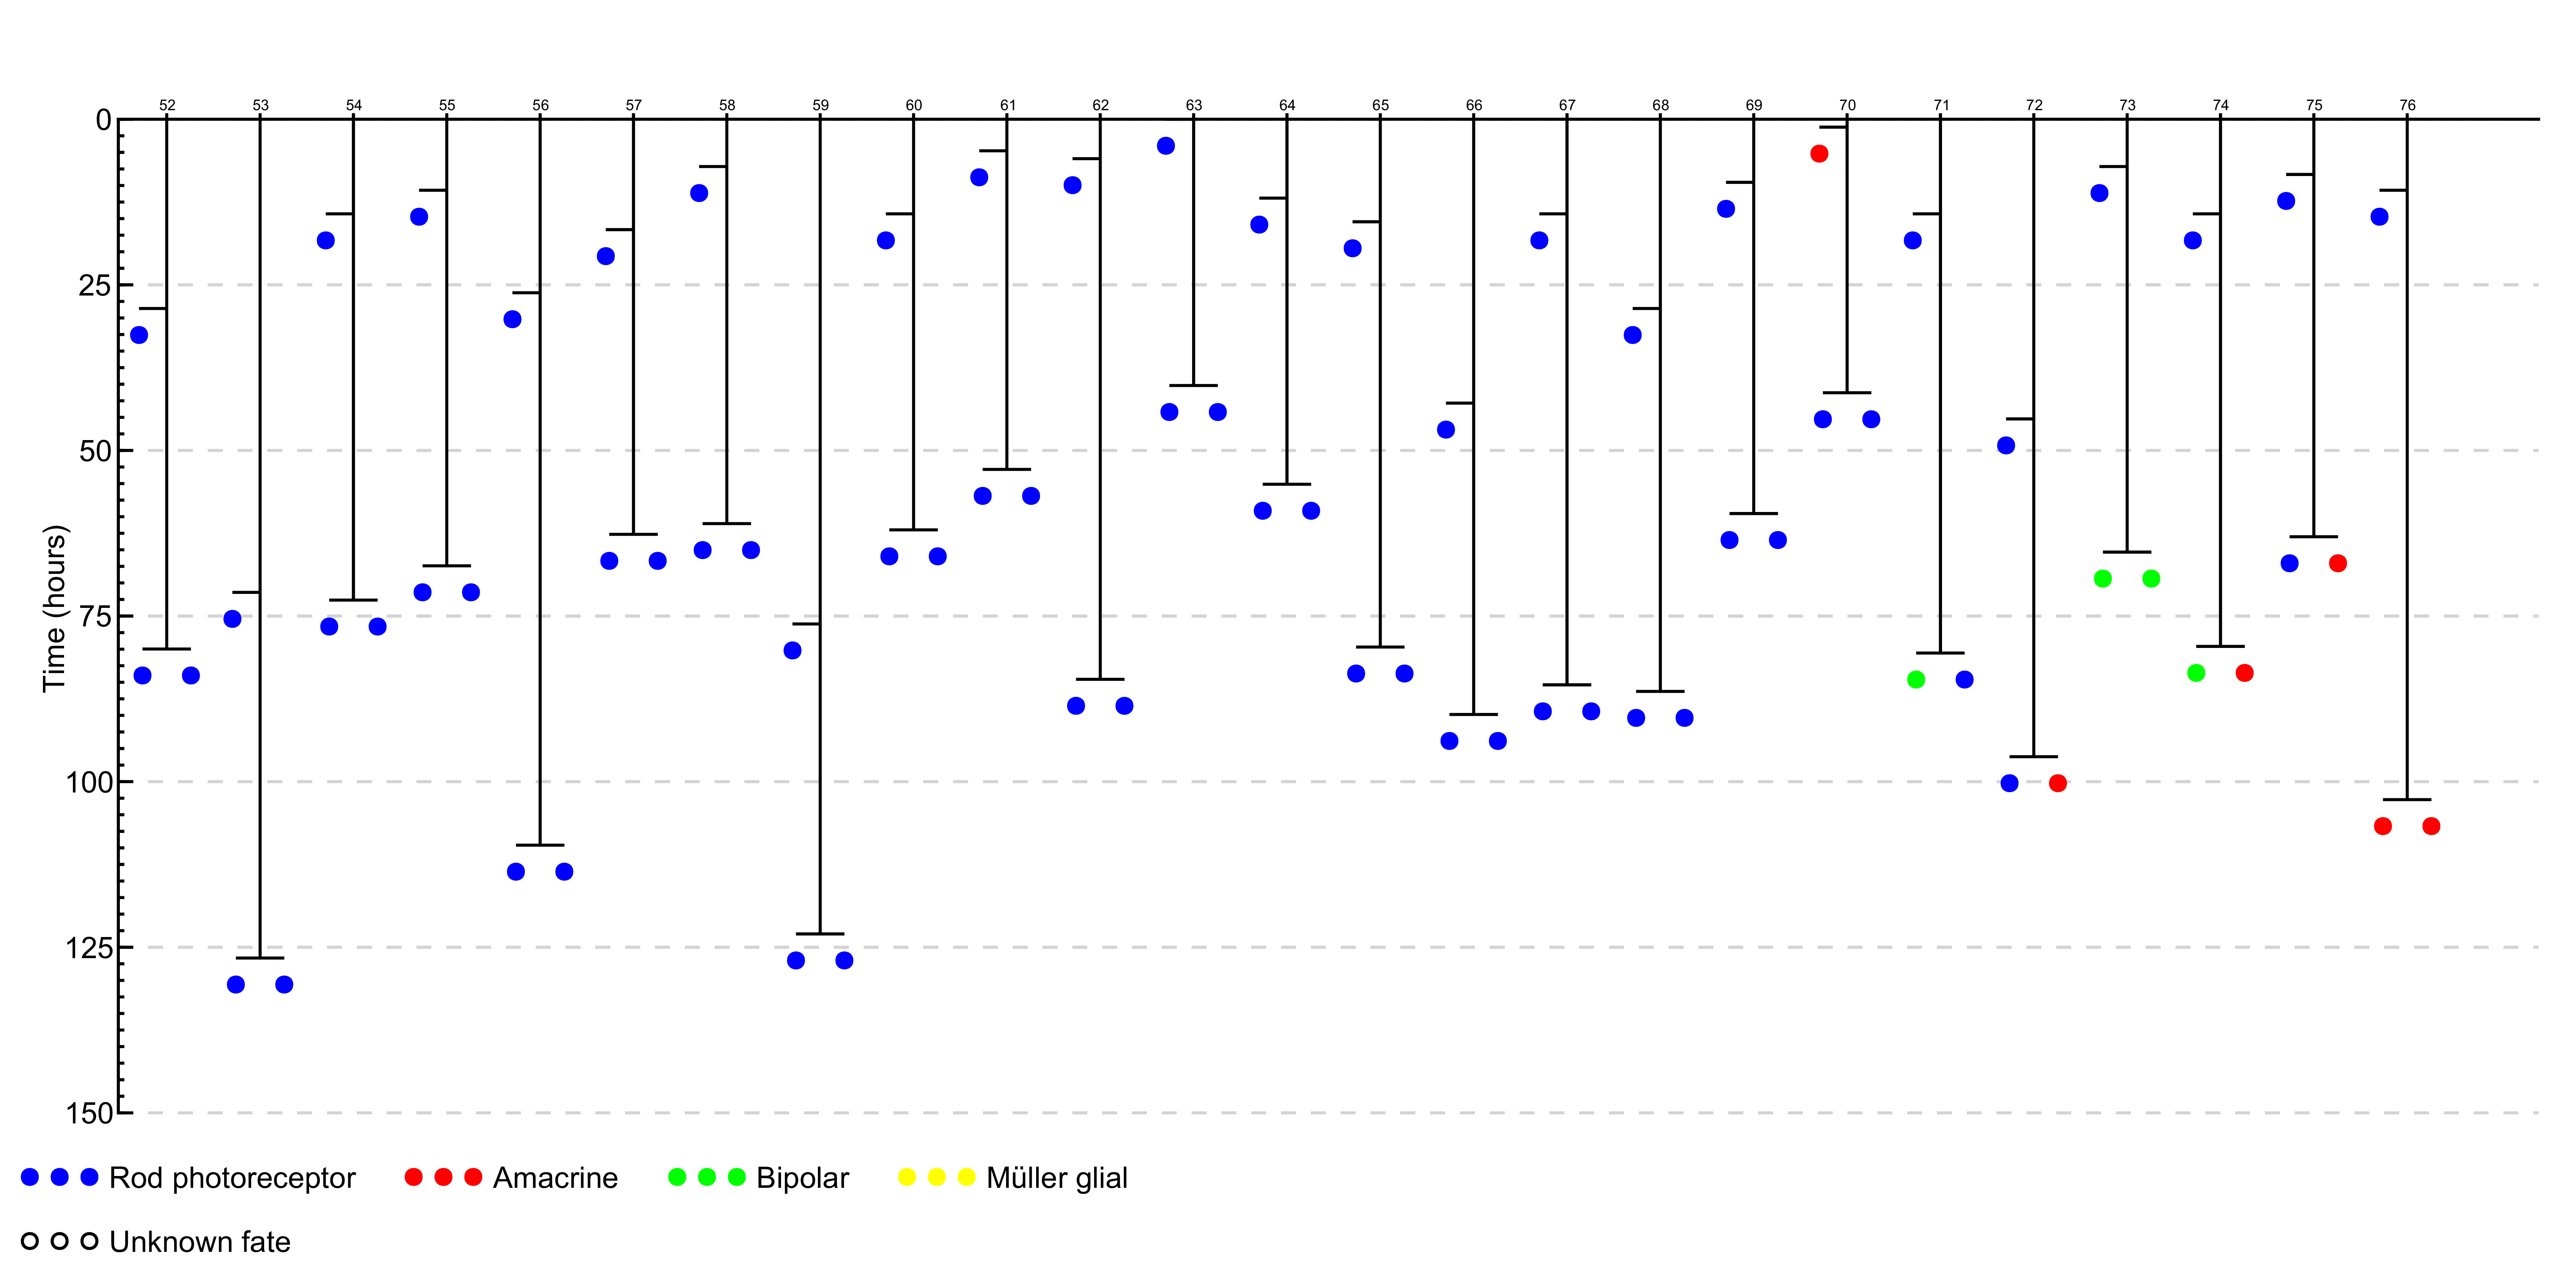
\includegraphics[width=0.5\columnwidth]{retinalLineageData3}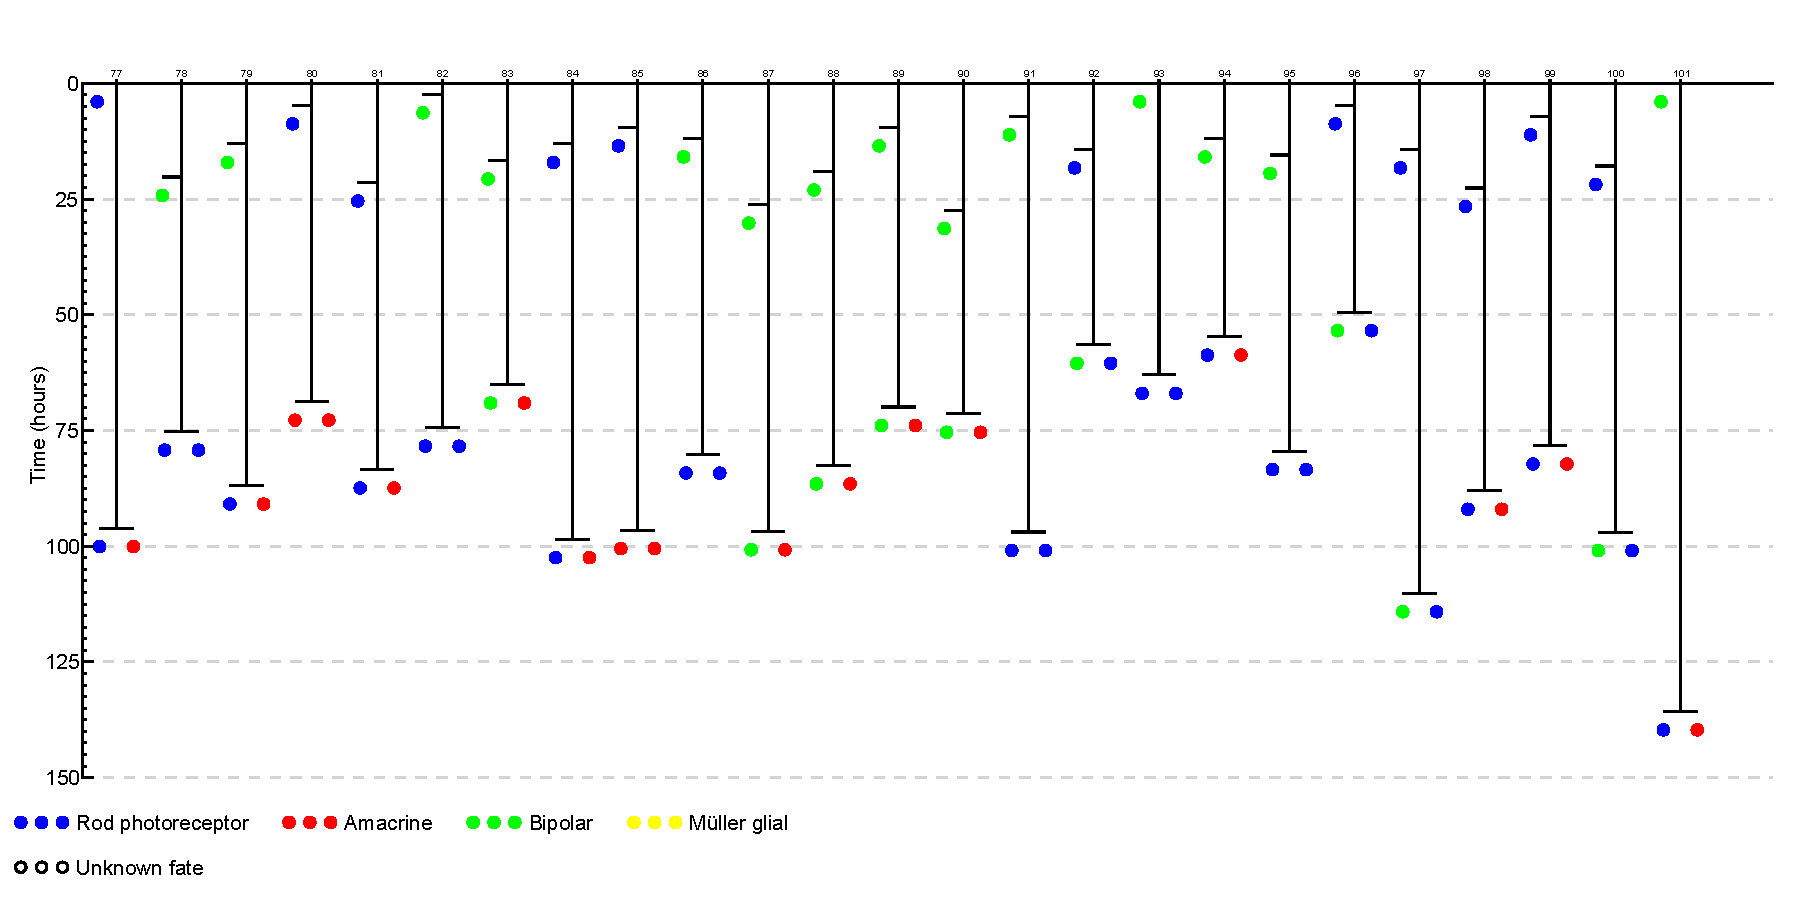
\includegraphics[width=0.5\columnwidth]{retinalLineageData4}

\begin{centering}
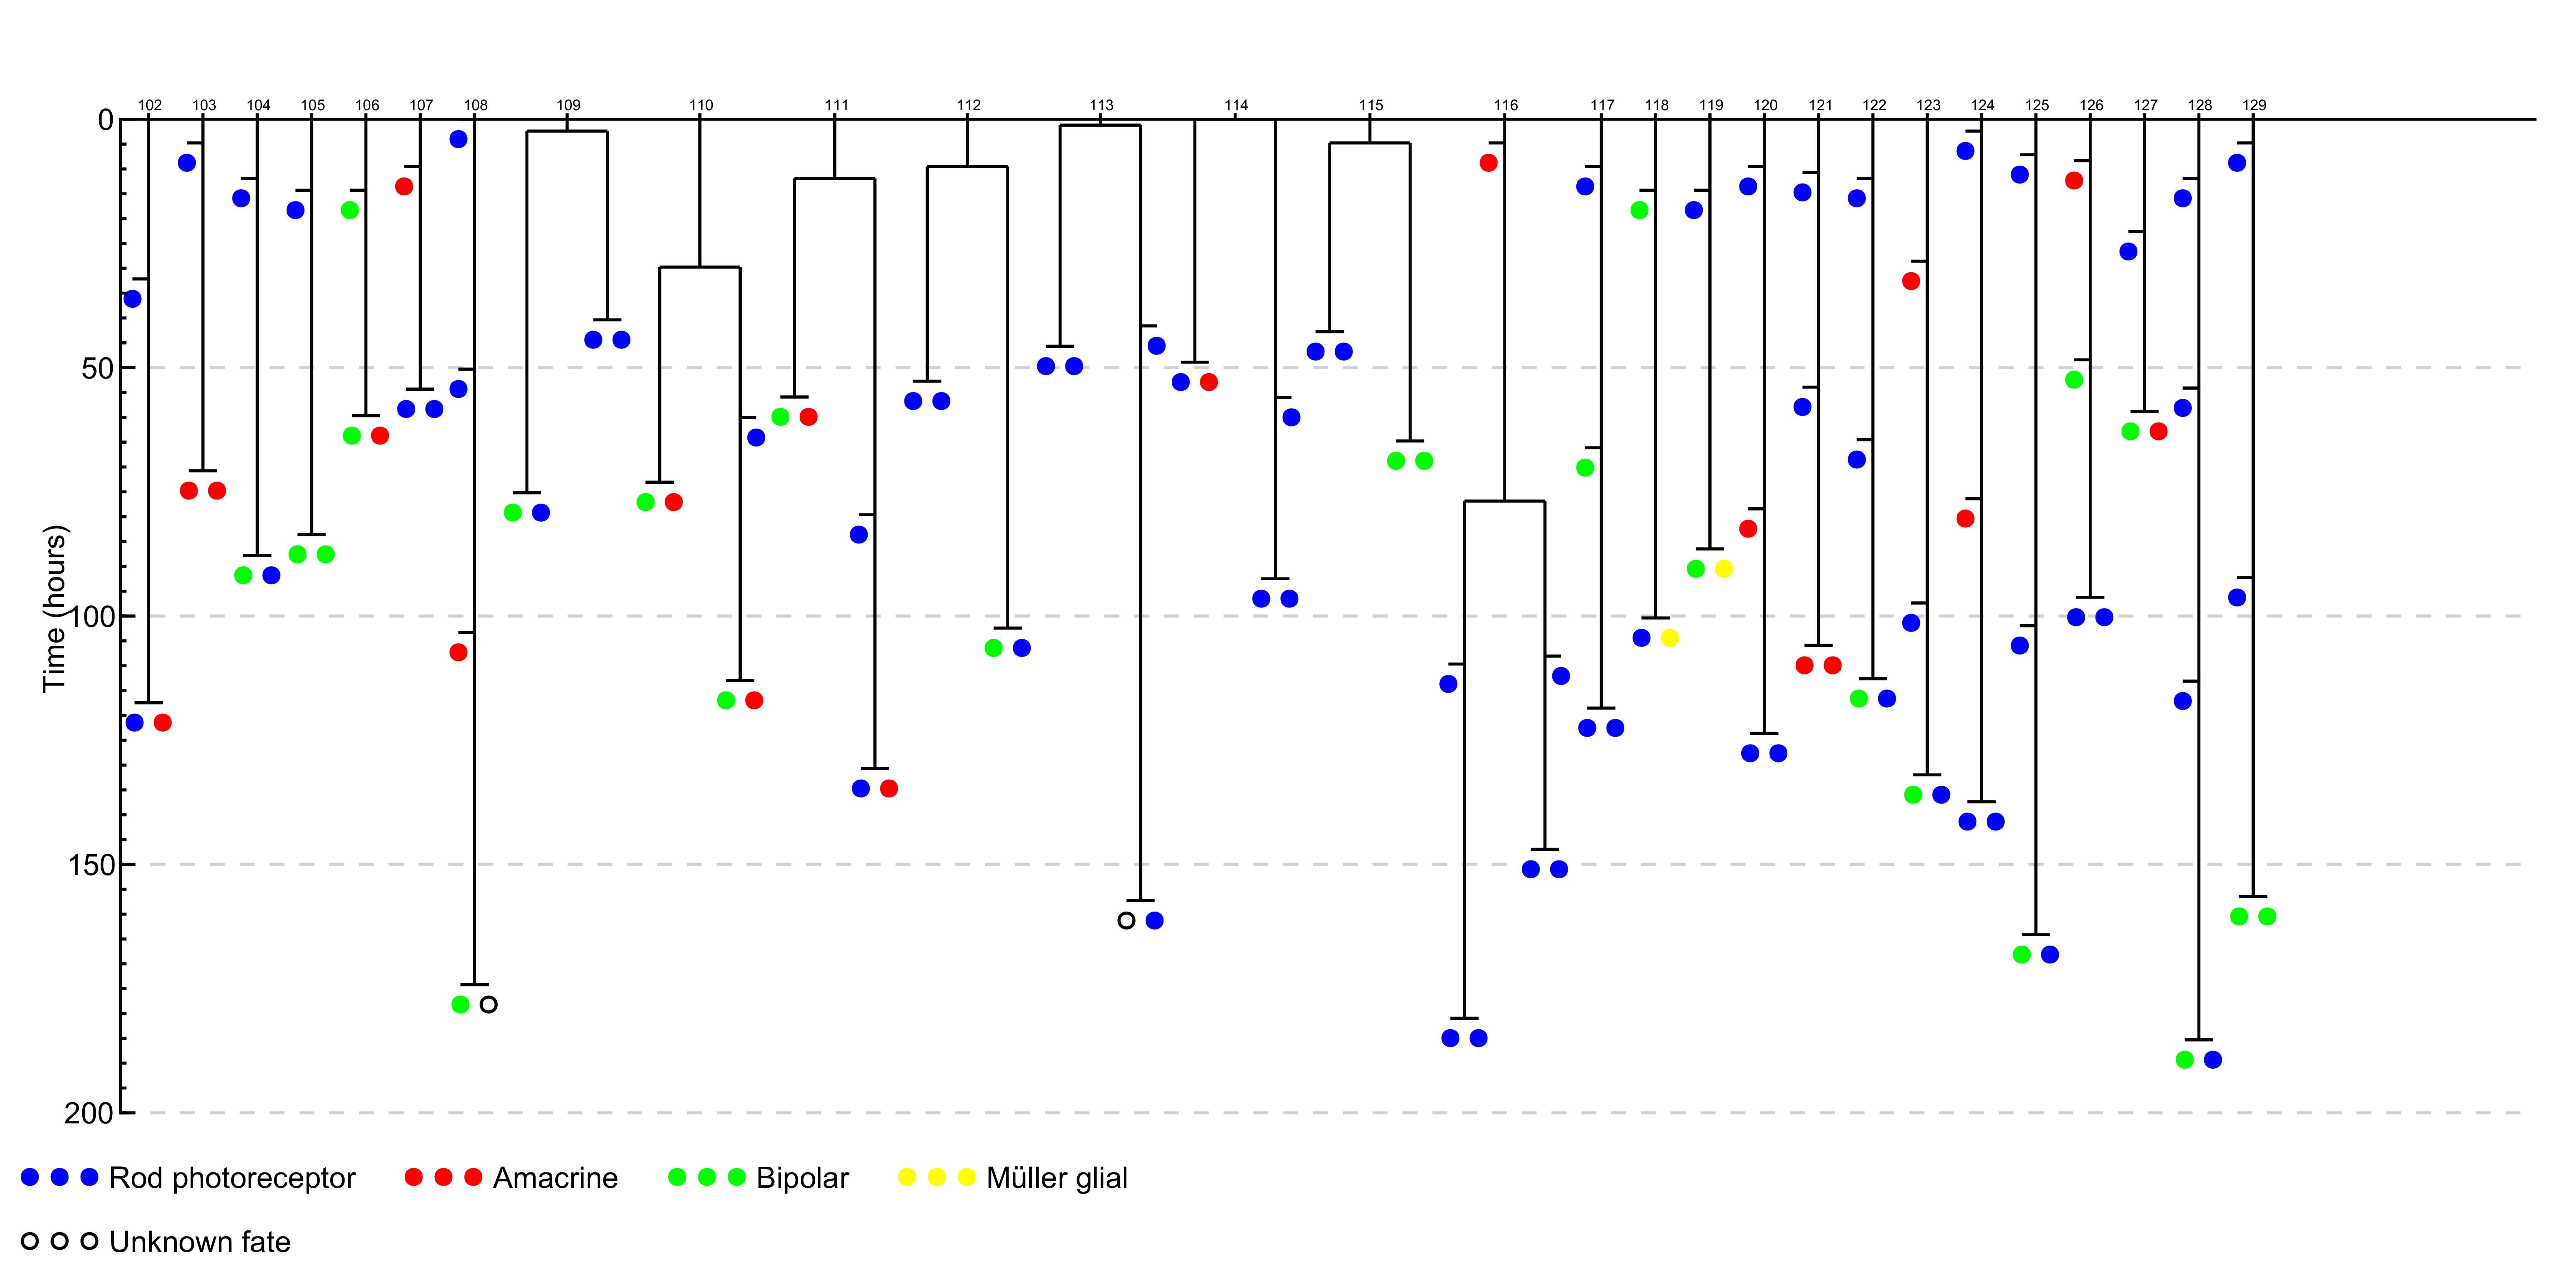
\includegraphics[width=0.5\columnwidth]{retinalLineageData5}
\par\end{centering}

\caption{\label{fig:rat-raw}The full dataset of all 129 reconstructed lineages
in this study. Different cell types are color-coded, as indicated.}


\end{figure}



\section{Stochastic progenitors}

Using the reconstructed lineage data, we first asked how E20 RPCs
achieve the required balance between proliferation and differentiation.
We analyzed the different modes of cell division observed in the overall
population. For the ensemble of clones with three or more cells, for
which the lineage trees were fully reconstructed, the first division
must inevitably involve the survival of at least one progenitor. Therefore,
to obtain an unbiased statistical measure of the modes of cell division,
we examined the lineage trees of the clones with three or more cells
after their first division. Out of 199 divisions recorded, 44 (22.1\%)
were self- renewing divisions that produced an RPC and a differentiating
daughter (P/D divisions), whereas 144 (72.4\%) were terminal, giving
rise to two differentiating daughter cells (D/D divisions). Such terminal
divisions, although symmetric in the sense that both daughters exit
the cell cycle, could also be symmetric or asymmetric in the sense
that the daughter cells may be of the same or different types, respectively.
To avoid confusion, we shall generally refer to all terminal divisions
as D/D divisions, regardless of whether the two daughter cells adopt
the same or different fates. Finally, only 11 divisions (5.5\%) were
found to generate two RPCs (P/P divisions). Since the P/P mode of
division accounts for only a small fraction, these results indicate
that differentiative (D/D) divisions, and to a lesser extent self-
renewing (P/D) divisions, are the major source of neurogenesis and
gliogenesis in the perinatal retina, at least in culture. Although
these figures point unambiguously to the predominance of D/D and P/D
divisions at this stage of retinogenesis, they leave open the question
of whether the balance of these division modes changes significantly
over the timecourse of the experiment. To investigate this, we compared
the second divisions of each lineage tree with those of the third
and beyond. Of the 131 second divisions, 95 were D/D (72.5\textpm{}7.4\%),
31 were P/D (23.6\textpm{}4.3\%) and five were P/P (3.8\textpm{}1.7\%);
errors are estimates based on Poisson statistics for the counts, i.e.
(count\textpm{}count)/total counts. This leaves 68 third and beyond
divisions, of which 49 were D/D (72.1\textpm{}10.3\%), 13 were P/D
(19.1\textpm{}5.3\%) and six were P/P (8.7\textpm{}3.6\%). The difference
between the second and third divisions remains within the error bars,
indicating that over the timecourse of the experiment the ratio of
D/D, P/D and P/P divisions remains roughly constant.

The similarity in the relative division ratios between one generation
and the next suggests that the balance between proliferation and differentiation
of a RPC is not influenced by the fate of its parent. In other words,
the division mode of a given RPC (P/P, P/D or D/D) is unpredictable
and, in this sense, stochastic. To test this possibility directly,
we compared the chance of finding a clone of size $n$ in the experimental
dataset with that predicted by a model in which RPCs divide with a
fixed probability $P_{PP}=0.055$ of adopting the P/P cell fate, $P_{PD}=0.221$
of adopting the P/D cell fate and $P_{DD}=0.724$ of adopting the
D/D cell fate (\figref{rat-clone-size}). Strikingly, the results
of a Monte Carlo simulation show an excellent agreement with the experimental
data. Moreover, for the same number of clones with three or more cells
(129), the model predicts an approximately normal distribution for
the total number of cells across all clones, with an average of 487
and a standard deviation of 22. This is again consistent with the
465 observed in the experiment.

\begin{figure}
\begin{centering}
\includegraphics[width=0.65\columnwidth]{F2\lyxdot large}
\par\end{centering}

\caption{\label{fig:rat-clone-size}The observed clone size distribution is
reproduced by a stochastic model. The data points (blue) show the
size distribution associated with the 129 clones with three or more
cells. If we assume that the balance between proliferation and differentiation
is determined stochastically, with RPCs dividing with a fixed probability$P_{PP}=0.055$
of adopting the P/P cell fate, $P_{PD}=0.221$ of adopting the P/D
cell fate and $P_{DD}=0.724$ of adopting D/D cell fate, we obtain
the clone size distribution given by the red curve. The error bars
on the theoretical curve denote 95\% confidence intervals and are
a result of the finite sample size. Since the probability of adopting
the P/P cell fate is small, the size distribution is close to exponential,
reflecting the fact that the majority of clones can be described by
a sequence of asymmetric P/D divisions terminating in a D/D division.}


\end{figure}


These results suggest that, at least from E20 and over the timecourse
of the experiment in vitro, the mode of division of RPCs is stochastic
with biased probabilities that remain approximately fixed. Our previous
findings that the size distribution of clones that develop in clonal-density
cultures is very similar to that of clones that develop \emph{ex vivo}
in retinal explants (Cayouette et al., 2003) suggest that this is
not a pathology associated with culture conditions. In addition, because
the RPCs are cultured at clonal density, these results suggest that
biased probabilities do not depend on specific environmental cues.


\section{Independence of division and fate choice}

We next considered whether the time that an RPC spends in the cell
cycle correlates with cell fate choice. We directly measured the cell
cycle time of RPCs generating all observed combinations of daughter
cell pairs by counting the elapsed time between the mitosis that produced
these cell pairs and the previous one. We found no significant difference
in cell cycle time of divisions producing any of the combinations
observed (\figref{rat-cycle-fate-and-dist}, left), indicating that
cell cycle time does not correlate with any particular cell fate decision. 

\begin{figure}
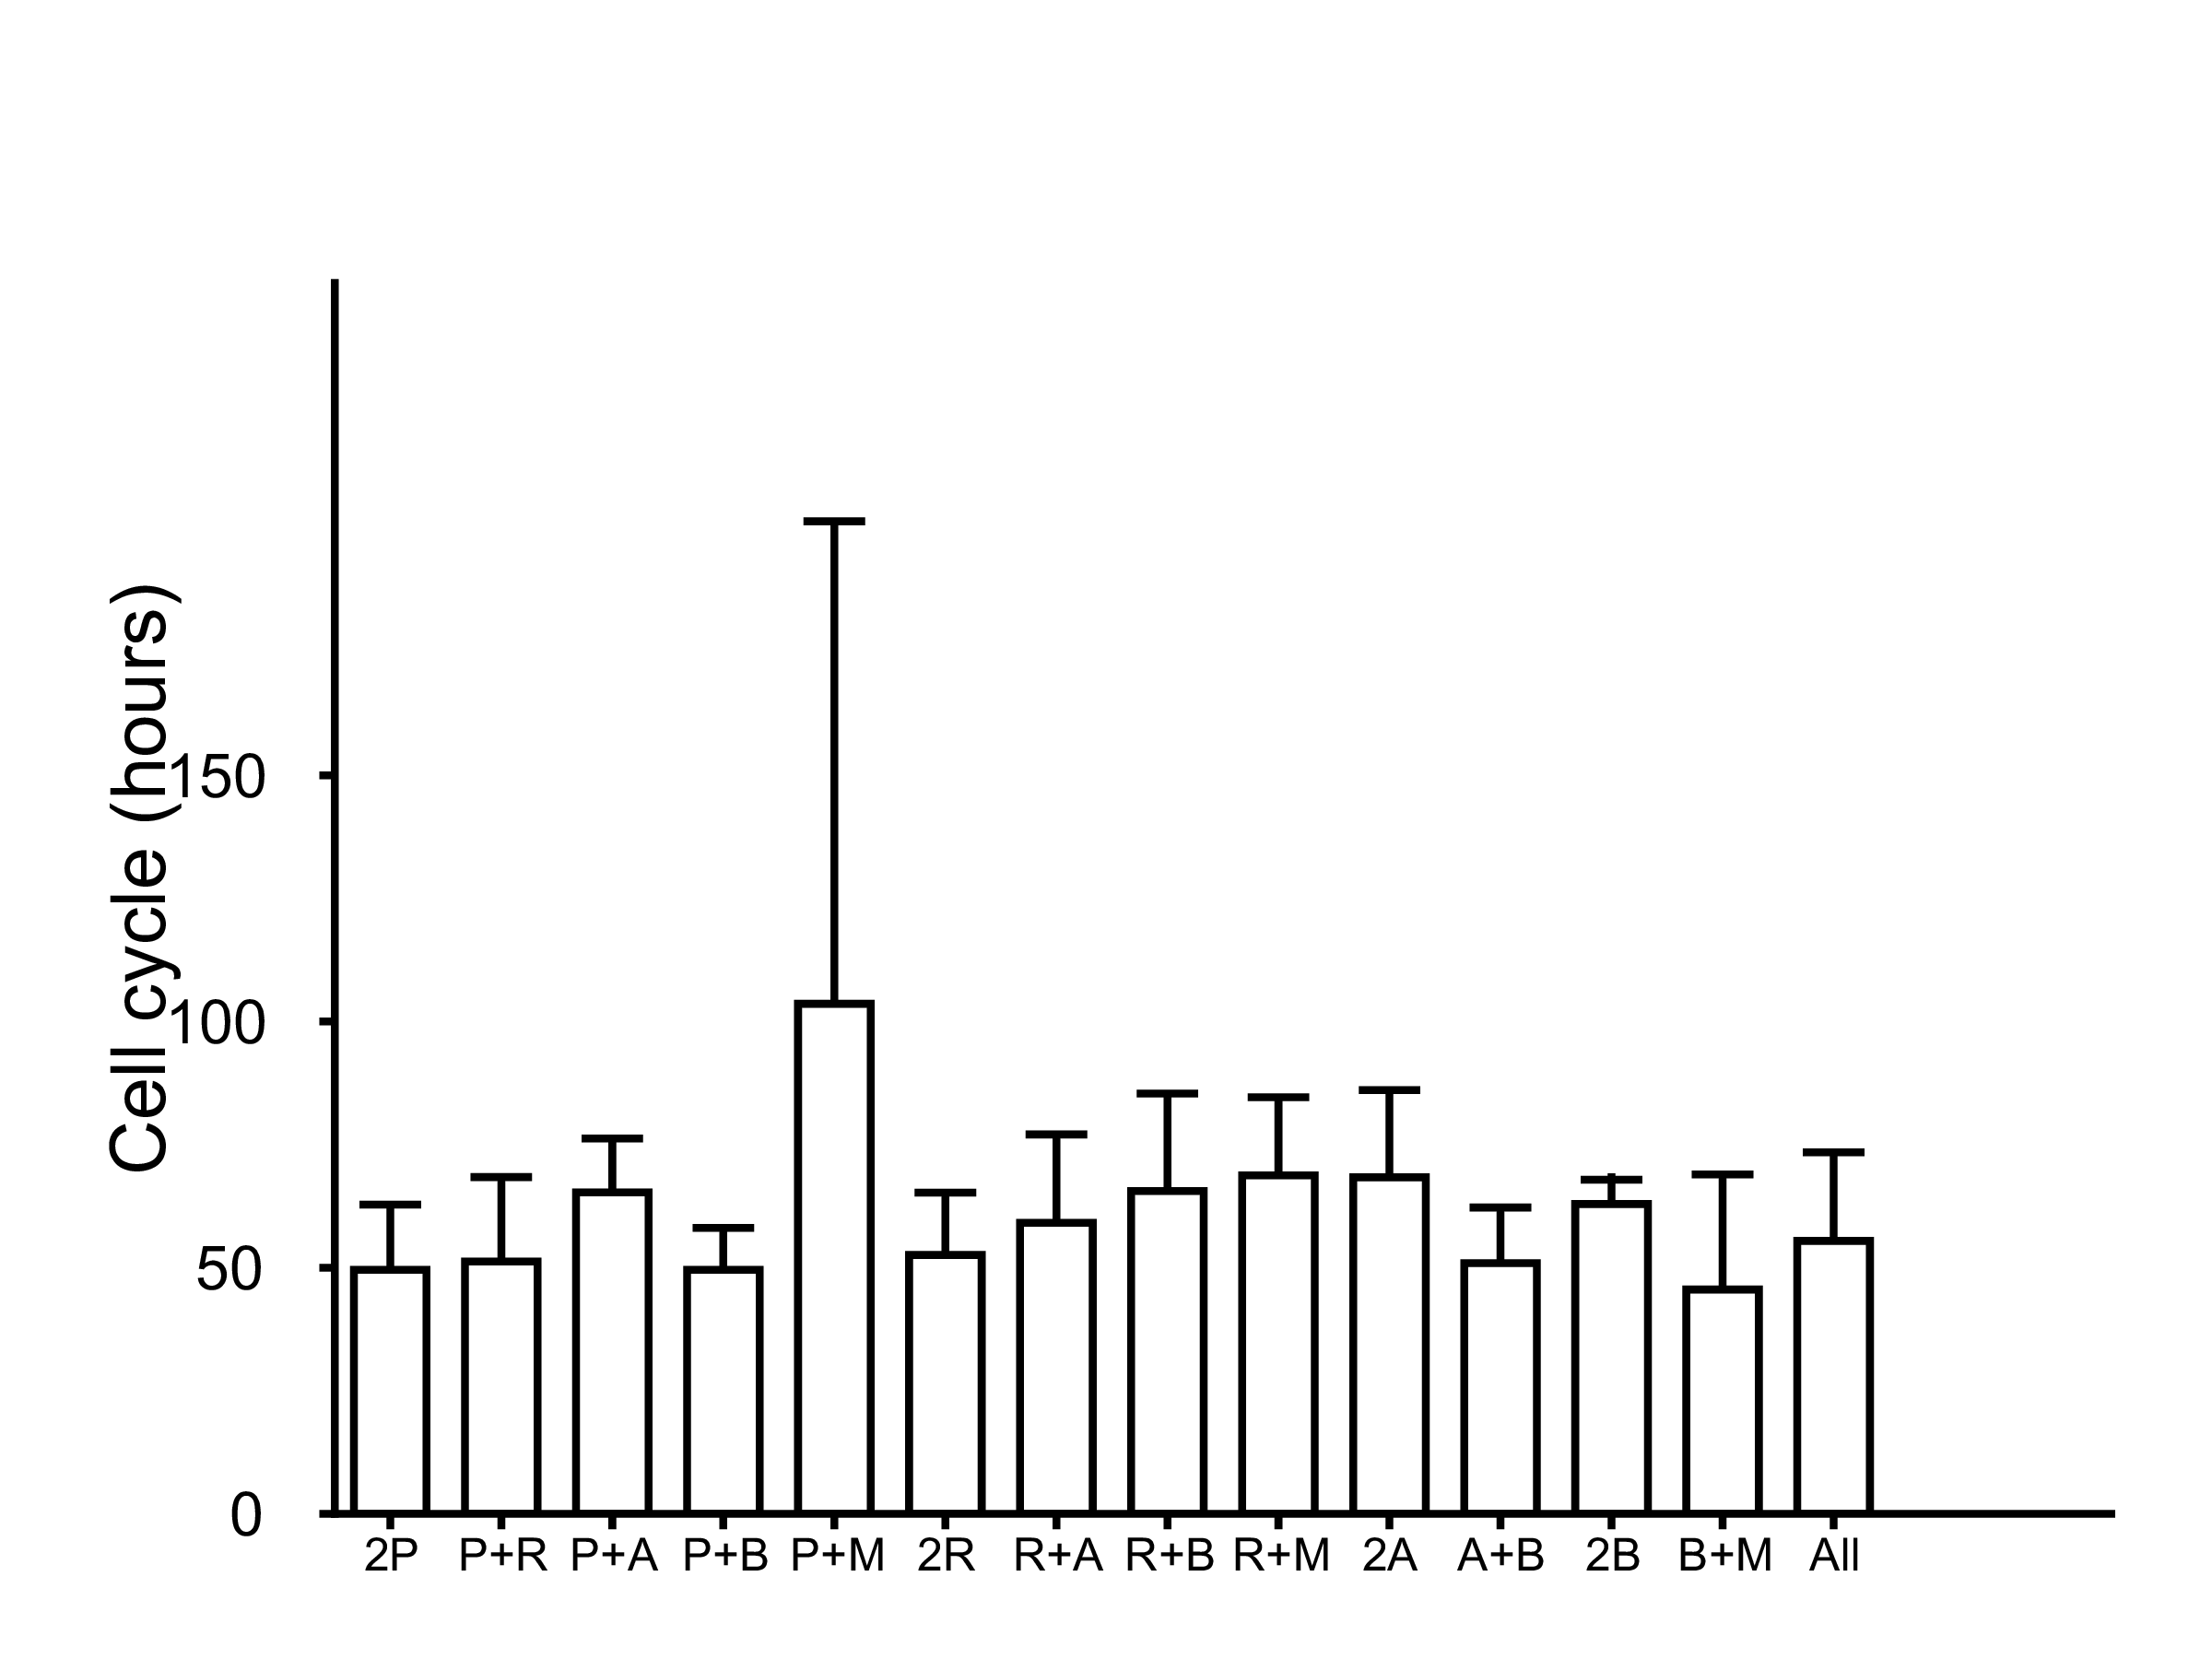
\includegraphics[width=0.5\columnwidth]{cycleLengthvsFate}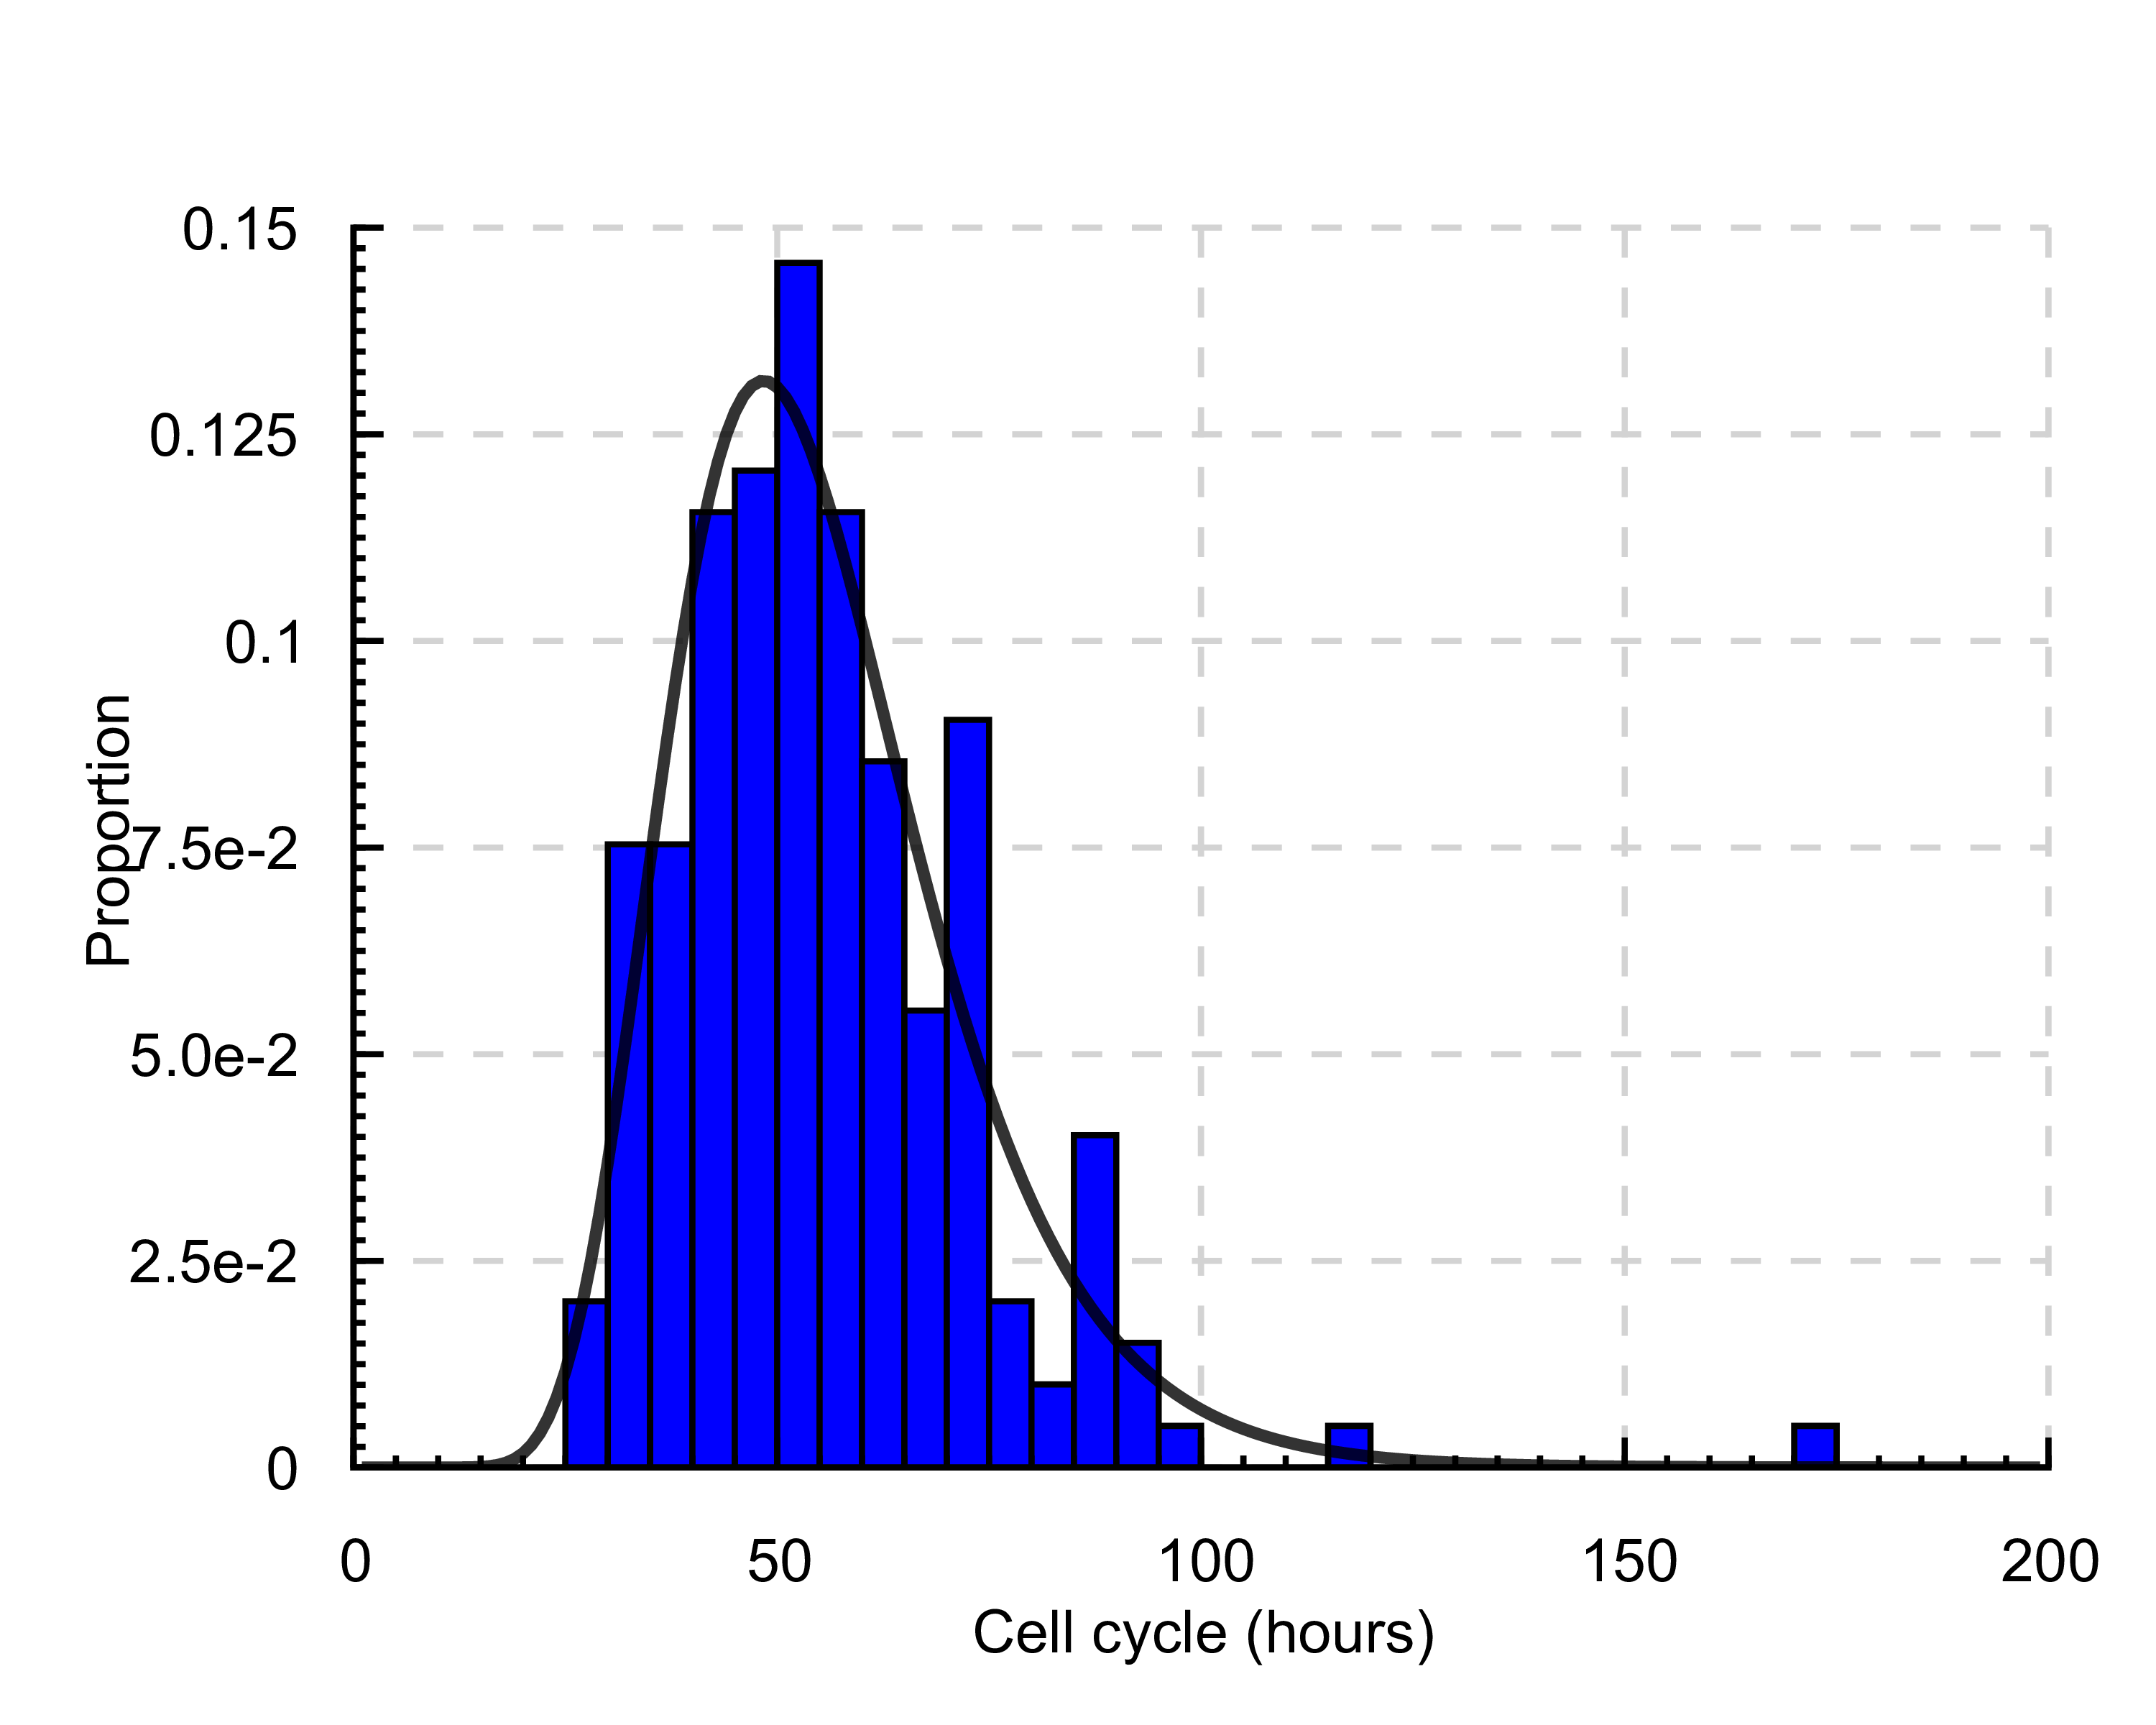
\includegraphics[width=0.5\columnwidth]{cycleLengthHist}

\caption{\label{fig:rat-cycle-fate-and-dist}\textbf{Left}: average cell cycle
time (mean + population s.d.) of RPCs generating all the different
combinations of daughter cell pairs observed in this study. A, amacrine;
B, bipolar; M, M�ller; P, progenitor cell; R, rod photoreceptor. \textbf{Right}:
observed cell cycle time distribution (bars) together with a log-normal
fit (line). The mean is 56.0 hours and population s.d. is 18.9 hours.}
\end{figure}


Grouping the data from all cell divisions, independent of fate, we
found that the cell cycle time was variable within the RPC population,
with an average of 56.0 hours and a population standard deviation
of 18.9 hours. The distribution of cell cycles were well approximated
by a log-normal distribution (\figref{rat-cycle-fate-and-dist}, right).
Also, upon comparing the cell cycle times of any consecutive divisions
($n=61$), we found no evidence of correlation (\figref{rat-cycle-correlations},
left). However, when we measured the difference in cell cycle times
of all the daughter cells of P/P divisions (n=21), we found a standard
deviation of 17 hours, significantly smaller than $\sqrt{2}\times19$
hours, where 19 hours is the standard deviation of all cell cycle
times, which would be expected if their division times were uncorrelated.
This result suggests a degree of synchrony in the timing of division
of sister RPCs that might contribute to the general timing of retinogenesis.

These results suggested that RPCs do not depend on mechanisms that
count cell cycle time or the number of divisions to regulate lineage
termination. By refining the stochastic model associated with the
modes of division to include a log-normal spectrum of division times
(consistent with the experimental data), a Monte Carlo simulation
shows lineage termination times that agree with the overall distribution
of termination times obtained experimentally (\figref{rat-cycle-correlations},
right). Together, these results indicate that the timing of lineage
termination, and thus the overall size of the retina, may be explained
simply as the result of a combination of stochastic fate decisions.

\begin{figure}
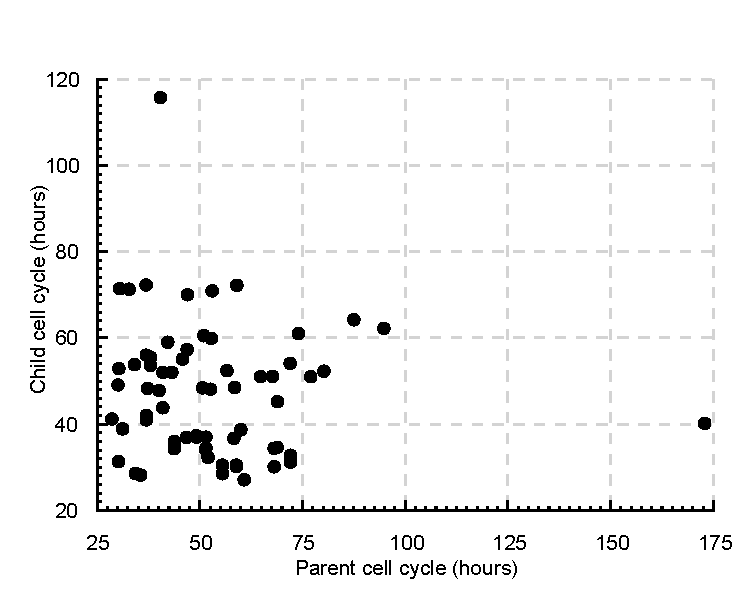
\includegraphics[width=0.5\columnwidth]{divisionSynchrony}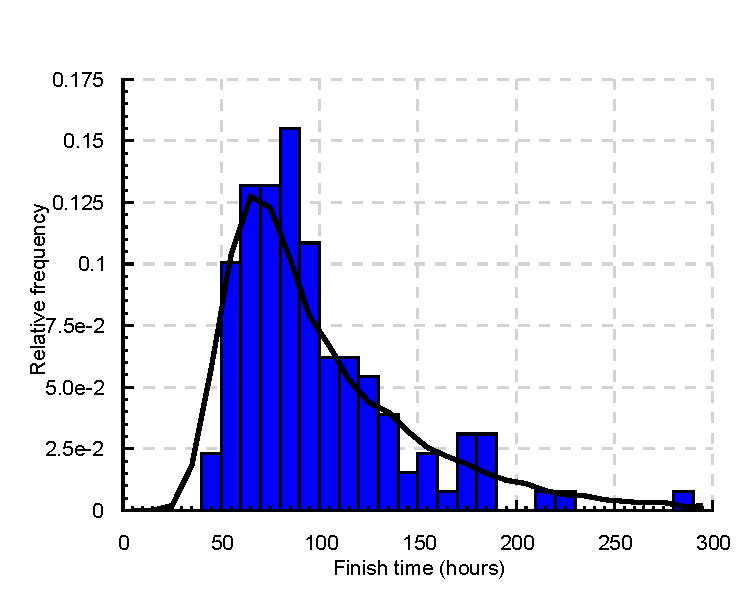
\includegraphics[width=0.5\columnwidth]{finishTimesHist}

\caption{\label{fig:rat-cycle-correlations}\textbf{Left}: cell cycle times
of daughter RPCs plotted against the cell cycle times of their mothers
reveals no discernable correlation. \textbf{Right}: The data (bars)
show the measured distribution of lineage termination times. The line
shows the predicted distribution of lineage termination times for
a stochastic model in which the ratios of proliferation and differentiation
are the same as that defined in \figref{rat-clone-size}, and the
distribution of cell cycle times is taken to be log-normal with parameters
chosen to fit the experimental data in \figref{rat-cycle-fate-and-dist}.
The curve is obtained from a Monte Carlo simulation. This comparison
provides a sensitive test of the stochastic model, as deviations from
it are magnified through repeated application.}
\end{figure}



\section{Almost stochastic cell fate specification}

Previous experiments have shown that rod photoreceptors represent
73\% of all cells in the mouse retina in vivo (Young, 1985), and,
similarly, 73.8\% of all cells produced in the reconstructed lineages
were RPh. How is such an imbalance of cell type production achieved?
It could be that multipotent RPCs are largely biased toward producing
photoreceptor cells at each division. Alternatively, it could be that
a subset of RPCs becomes committed at some point in their lineage
to generate exclusively RPh cells, thereby greatly increasing the
number of RPh cells that can be produced from the same RPC pool size.
Although differences may exist between in vivo and in vitro lineage
progression, the continuous observation of RPC lineages performed
in this study allowed us to begin to address this problem directly.

To benchmark the experimental data, we used a model in which both
the balance between proliferation and differentiation, and the differentiated
cell type, were chosen at random, with probabilities fixed by the
measured average of each cell type produced in the clones (i.e. the
probability that a differentiated cell adopts an RPh fate is given
by $P_{RPh}=0.738$, etc.), independent of the fate of its sister,
parent or any other cell in its lineage. Then, to seek evidence for
lineage specification, we looked for the simplest statistical measure
focusing on the correlation of cell fate between consecutive generations
of cells. Specifically, we explored the correlation between the fates
of two consecutive lineage-related divisions. From a total of 201
qualifying divisions from within the 129 clones, the number that generated
a given cell fate versus the fate of the sister of the parent cell
is shown in \tabref{rat-comparison}.

\begin{table}
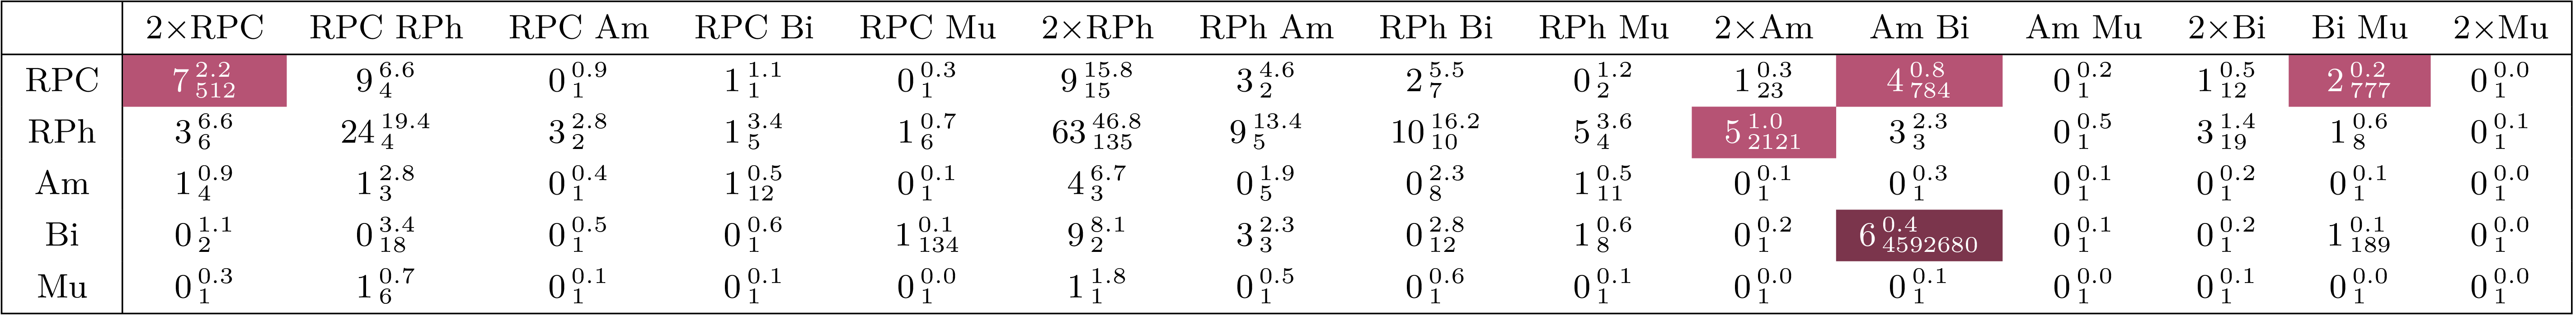
\includegraphics[width=1\columnwidth]{comparisonTable}

\caption{\label{tab:rat-comparison}Each entry displays three quantities for
a given triplet of cells generated by two consecutive lineage-related
divisions. The number in a large font denotes the observed frequency
of the event. The superscript represents the prediction made by a
stochastic model in which the relative division probabilities leading
to proliferation and differentiation are set by the parameters shown
in \figref{rat-clone-size}, and the relative probabilities of the
differentiated cell types is specified at random with $P_{RPh}=0.738$,
$P_{Bi}=0.128$, $P_{Am}=0.106$ and $P_{Mu}=0.028$, corresponding
to the observed frequencies of the population. The subscript indicates
the quality of the agreement between the experiment and the stochastic
model, expressed as the number of experiments (each involving 201
aunt/niece triplets) one would expect to perform before seeing a statistical
fluctuation of this magnitude or greater. This figure should be compared
with the total number of entries (75) \textendash{} much greater than
this is a sign of a genuine outlier. Outliers that stand at three
and four standard deviations are light and dark red, respectively.
For example, the entry at (RPh, RPCRPh) represents events involving
two consecutive P/D divisions in which both differentiated progeny
adopted the RPh cell fate. Out of the 201 entries, from the table,
we find that such an event occurred 24 times. This compares to the
19.4 average predicted by the stochastic model. From the subscripted
number, we see that one would expect to see a departure from the theoretical
prediction of this magnitude or larger in one out of four experiments
owing to statistical fluctuations, i.e. the observed data are entirely
compatible with the statistical model. By contrast, if we look at
the entry (Bi, AmBi), we expect to see an average of 0.4 events out
of 201, whereas the data show six. Such a fluctuation would arise
in typically only one out of 4.6 million experiments, i.e. the observed
data are clearly incompatible with the statistical model as defined.}


\end{table}


From the raw experimental data several features emerged. First, there
were a number of entries for which no examples were found. Second,
several of the entries were large, including the putative RPh lineage
(RPh, RPhRPh) and (RPh, RPCRPh). However, by themselves, neither of
these observations provides conclusive evidence for recurring lineage
patterns. Since the data were acquired from only a limited number
of clones, if certain lineage combinations were rare we might indeed
expect to record no examples in the limited data set. Moreover, if
cell fate choice were stochastic, but heavily biased toward RPh fate,
we might find large entries in a seemingly RPh-specific lineage that
derived simply by chance and not from early lineage commitment. Thus,
to calibrate the data we used the stochastic model as a benchmark.

In Table 2, we also show the expected number of entries for an experiment
with the same number, 201, of qualifying cell divisions if cell fate
outcome were random. In addition, we have included the number of experiments
(each with 201 qualifying cell divisions) that we would expect to
have to perform to find at least one experiment with a statistical
fluctuation that was equal to, or larger than, the actual measured
experimental value. If this number is greatly in excess of the 75
possible fate outcomes in the table, we can consider the entry as
an outlier, seemingly inconsistent with the random hypothesis. If,
by contrast, it lies within 75, any departure of the experimental
value from the expected result can be explained simply as a fluctuation
associated with small-number statistics. 

From this analysis, we noticed, for example, that the large entry
for (RPh, RPCRPh) lies well within the expected range for the random
model, along with the vast majority of other entries, consistent with
such combinations being produced stochastically. However, from the
75 entries, five outliers were identified, which stand at three or
more standard deviations from the expected average: (RPC, RPCRPC);
(RPh, AmAm); (RPC, AmBi); (RPC, BiMu); and (Bi, AmBi). Such outliers
should appear at most only once per 370 entries. Moreover, the (Bi,
AmBi) entry lies beyond five standard deviations and indeed would
only be expected to appear around once in 4.6 million experiments.
Clearly, these cannot be explained simply as a number fluctuation,
and although the chronology of cell type production might somewhat
influence lineage selection, these results suggest that, in addition
to stochastic mechanisms, specific recurring lineages or lineage priming
may play a part in retinogenesis.


\section{Conclusion}

We studied rat retinal progenitors in culture, by reconstructing complete
lineage trees from time-lapsed imaging. We find a great deal of heterogeneity
in both size and composition of the resulting lineages, but which
can be almost entirely explained by a simple model of time-invariant
progenitors which undergo a stochastic process of division and fate
specification. Whilst there were outliers in the fate outcomes observed,
the results suggest that a great deal of the development is regulated
intrinsically, but not stereotypically. Nevertheless, we are cautious
in interpreting the results, as they are in the context of cultured
cells at the late end of development. In the next chapter, we go on
to a \emph{in vivo} system which encompasses a much greater range
of the developmental program.


\chapter{How Stochastic Progenitors Build an Invariant Zebrafish Retina}

In the last chapter, we saw that retinal progenitor cells (RPCs) in
culture can be modelled by a simple stochastic process of independent
and time-invariant progenitors with fixed proportions for fate outcomes.
Aside from the occasional correlation in lineage trees which are statistically
significantly deviant from the model, a more serious problem is that
the system is \emph{in vitro}, with no real tissue being built and
so no potential for cell-cell interactions to become manifest. In
this chapter, we move to consider a system in live zebrafish embryos,
which via a battery of genetic labelling techniques, also allow different
ways to trace lineage trading detail for data volume . However, given
the complexity of the system and difficulty of obtaining sufficient
data, the model will be necessary more descriptive than prescriptive.
In particular, we have only found a possible model of relative simplicity,
rather than the unique and most simple model possible.

This chapter draws significantly from {[}cite{]}; the experimental
work was primary by JH, and ADA, the manuscript by WAH and data analysis
by GZ and BDS and discussions with MC. However, we have elided detailed
discussion of the experimental methods and their validation (which
in itself was a year-long project for the experimentalists), and focus
on the clonal analysis. We again refer the interested reader to the
published work.


\section{The developing zebrafish retina in space and time}

The retina is a pseudo-stratified epithelium, with progenitors being
elongated with processes that attached each cell to a basal membrane.
The fully developed retina has distinct layers of cell types (\figref{zf-retina-anatomy}),
but progenitors can, and tend to, move apically before dividing, and
the daughters will move basally to settle into the correct layer.
Over a short period of time (20--72 hpf) the retina grows by a factor
of approximately 12 in cell number, by both expansion in volume and
increase in density of cells. 

\begin{figure}
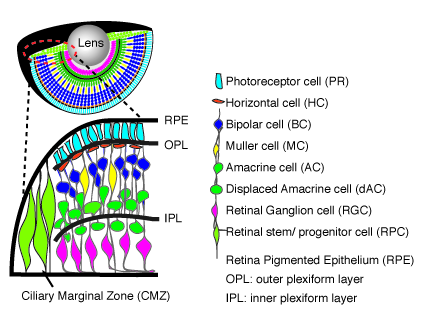
\includegraphics[width=0.3\textwidth]{zf-anatomy-schematic}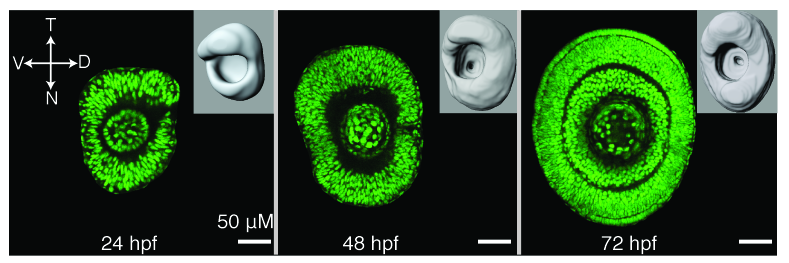
\includegraphics[width=0.7\textwidth]{zf-saggital-sections}\caption{\label{fig:zf-retina-anatomy}\textbf{Left}: schematic of the developed
retina; the ciliary margin zone (CMZ) contains adult stem cells which
continue to grow the eye as the fish grows through adulthood. \textbf{Right}:
Representative images of the sagittal sections and the created retina
surfaces (inserts) at distinct developmental stages; note the distinct
asymmetry present at the intermediate phase (24--32 hpf) across the
ventral-dorsal plane.}
\end{figure}


From previous works (Hu and Easter, 1999; Neumann and Nuesslein-Volhard,
2000), it is known that a wave of differentiation progresses from
central to peripheral and nasal to temporal around the retina. Given
the asymmetry observed early (24 hpf) in the retina (\figref{zf-retina-anatomy},
right), it seems natural to ask if there is actually a wave of proliferation
that proceeds the differentiation. To dissect this behaviour, we used
a transgenic fish which labels proliferating RPCs with destablized
Green Fluorescent Protein (GFP) to literally visualise the proliferation
wave (\figref{zf-fucci}). Counting the exact number of GFP-labelled
cells in each half of saggital sections, we see that the behaviour
of different locations only differ by their relative timing, whilst
recapitulating (broadly) the same raise and fall of labelled cells.
In particular, note that before the raise (understood to be the proliferation
wave) the number of labelled cells is constant, implying that the
progenitors are in a state of quiescence. This is consistent with
previous results showing that between 15--24 hpf RPCs have extremely
slow cell cycle times of about 40 hr on average (Li et al., 2000). 

\begin{figure}
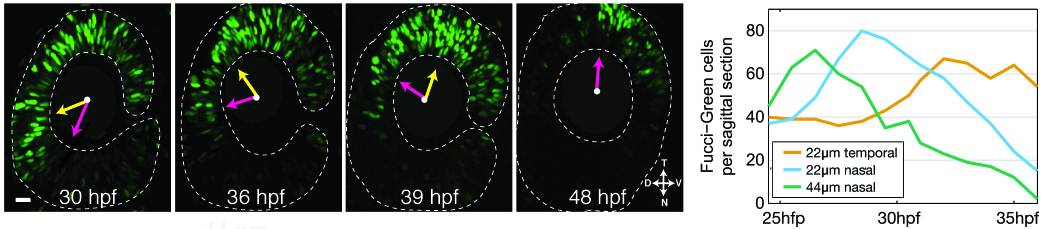
\includegraphics[width=1\textwidth]{zf-fucci}

\caption{\label{fig:zf-fucci}\textbf{Left}: Sagittal slices of a GFP-expressing
retina at various time points (yellow arrow points to region of highest
density of GFP and magenta arrow points to region of decline. \textbf{Right}:
Quantified GFP-positive cells over time by zone (nasal or temporal
zone) and depth (the distance between the most peripheral section
and the section of interests).}


\end{figure}


We thus have a picture of progenitors which are primed for action,
waiting for a signal. Upon receiving that signal, they rapidly divide
leading to a rise in number of progenitors. They then equally rapidly
differentiate leading to a decrease in the GPF-label. The wave takes
approximately 16 hours to progress from the central-most nasal side
to the outermost temporal side, after which the only remaining progenitors
reside in the CMZ.


\section{Stochastic progenitors, redux}

To understand what each progenitor is doing, we turn to clonal analysis.
The experimental system is another transgenic line involving a cross
between heat activated fluorescence (MAZe) and photoconvertable fluorescence
(Kaede). In particular, heat shock (usually performed at 8 hpf) gives
rise (with selection) to green fluorescent clones of one or two cells
at 20 hpf in the retina, of which one cell will be chosen at some
later time point (usually 24, 32 or 48 hpf) to be photoconverted to
red fluorescence by a UV laser. We thus have a choice of both induction
time and also imaging time. \figref{zf-clone-dists} shows some clone
size distributions obtained, displaying the expected heterogeneity
of clone size, but also some novel features not seen before in the
cultured system.

\begin{figure}
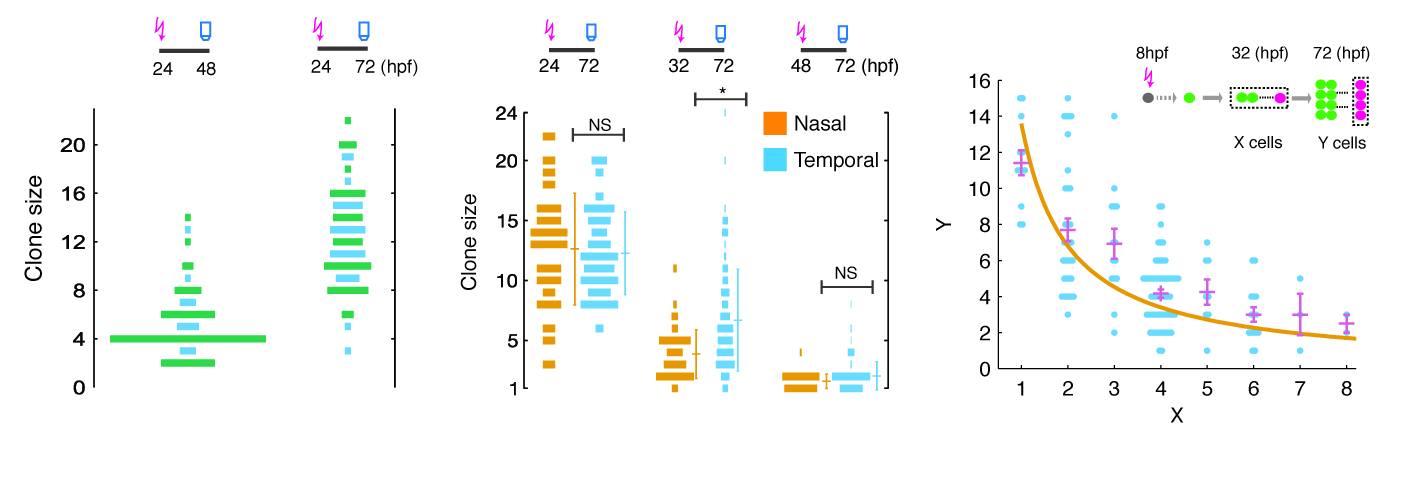
\includegraphics[width=1\textwidth]{zf-clone-dists}

\caption{\label{fig:zf-clone-dists}\textbf{Left}: Size distributions of the
clones induced at 24 hpf and recorded at 48 hpf (left) or at 72 hpf
(right), highlighting numbers of even (green) versus odd (blue) clones.
\textbf{Middle}: Size distributions of clones photoconverted at various
times. The mean and SD are indicated. \textbf{Right}: After photoconversion
at 32 hpf, the size of the resulting subclone at 72 hpf (y axis, depicted
as the magenta cells in the schematic shown in inset) is, on average,
approximately inversely correlated with the total size of the parent
clone at 32 hpf (x axis, shown as the enclosed green and magenta cells
in inset). The points show measurements from individual clones, while
the mean and SEM are shown in purple. If the fate of RPCs is independent
of clonally related cells, the average size of the subclone after
photoconversion is predicted to vary as $N/n$ where $N$ denotes
the average total clone size at 72 hpf and $n$ denotes the average
total clone size at 32 hpf. Indeed, the measured averages (purple)
are broadly consistent with this prediction (orange line).}
\end{figure}


First, we note that there is a significant lack of odd sized clones
from progenitors induced at 24 hpf and imaged at 48 hpf. This requires
divisions in this time window to be predominantly symmetric renewal
(PP) and sister RPCs should be synchronised --- a feature we had already
seen in the cultured rat retinal progenitors; there it was not a particularly
significant feature as PP divisions were rare. However, the lack of
scarcity of 6-cell clones indicate that divisions are not synchronised
beyond immediate sisters. Second, we see that this is no longer true
of clones spanning 24 to 72 hpf --- indicating asymmetric PD divisions
becoming important. But if we look at the 48 to 72 hpf clones, we
see that almost all divisions are terminal (DD), and furthermore with
4-cell clones greatly outnumbering 3-cell clones, there is almost
no PD either. Thus we conclude there being at least three separate
phases: initially highly proliferative, composed of synchronised PP
divisions, followed by a phase with significant PD divisions, finally
almost entirely DD. Given such a complex and particular sequence,
it is reasonable to ask if the progenitors are in fact stochastic
at all.

To rule out the possibility that progenitors are pre-programmed at
an early time (<20 hpf), but rather independently decide their fate,
we study a slightly subtle aspect of the clone distribution. In particular,
recall that our induction method actually creates clonally related
green cells at an early time (and upon selection is this restricted
to those of one or two cells in the retina at 20 hpf), but the subsequent
photoconversion only affects one of that clone and turns it red. We
thus look at the relation between the number of red cells at 72 hpf
and the number of green cells at 32 hpf (\figref{zf-clone-dists},
right). We note that the average number of red cells falls as the
inverse of the number of green cells, indicating that the RPCs index
their behaviour by a lineage-internal measure rather than a tissue-wide
signal. Furthermore, there is considerable variance --- if the size
of a clone is pre-programmed, then there would be almost no variance,
as later progenitors would know if they belonged to a small or large
clone. Thus, we see that progenitors are still stochastic, but with
evolving probabilities for chosing their fate.

Therefore, we will suppose that RPCs form a functionally equivalent,
equipotent cell population with evolving proliferative potential,
which is decoupled from the particular specification of individual
cell types. Through temporal and spatial correlations, we expect to
capture many aspects of the data, including correlations that might
otherwise require a causative hypothesis. Any residual correlations
between lineage and clone size are therefore a reflection of the histogenesis
of cell types or a signature of early fate specification. In this
paradigm, RPCs follow a (stochastic) developmental program, passing
from a near-quiescent phase to an active proliferating phase and finally
to a differentiating phase. The initiation and timing of this developmental
program is defined by the wave of proliferation that sweeps around
the retina, starting at the central nasal region and terminating at
the peripheral temporal zone. In the following, we will use the timing
of the first mitosis to define the start of the development program
within each lineage. This occurs at around 23 hpf in the central nasal
region, reaching the peripheral temporal region around 16 hours later.
For simplicity, we therefore suppose that RPCs enter their active
phase at a uniform rate, expecting that deviations from this will
be beyond the resolution of the data. If we assume that, over the
period from 24 to 48 hpf, RPCs are limited to the proliferative phase,
measurements of the average clone size over this period suggest a
cell cycle time of ca. 6 hr, allowing approximately two rounds of
symmetrical cell division. (Anticipating the results of the live-imaging
study, our simulations are actually performed with a shifted gamma
distribution, with a refractory period of 4 hr, mean of 6 hr, and
width of 1 hr.) In addition, the lack of odd-sized clones requires
a high degree of synchrony between division times of sister progenitors;
we assume a difference between sister cell cycles of around 1 hr,
normally distributed. Moreover, since the average clone size grows
12- to 13-fold over the period from 24 hpf to 72 hpf, we can deduce
that each progenitor at 48 hpf must go on to produce, on average,
three postmitotic cells. Thus, we may visualize a \textquoteleft{}\textquoteleft{}typical\textquoteright{}\textquoteright{}
clone to consist of two rounds of symmetrical (PP-type) division,
one round of asym- metrical (PD-type) division, and one round of terminal
(DD-type) division leading to the average 12-fold increase in average
clone size over the time course.

However, the variability in size of clones at 72 hpf, induced at 24
hpf, provides a strong signature of stochasticity in cell fate choice.
We therefore suppose that, within a lineage, the balance between proliferation
and differentiation is achieved through stochastic fate decisions,
with probabilities that vary through the developmental stages (\figref{zf-model}).
For simplicity, we assume these changes to occur instantaneously,
thus avoiding having to parameterize the change beyond just a single
time. In particular, since clones induced at 48 hpf involve very few
three-cell clones, PD divisions must be suppressed at these later
times. Thus, there must be at least two such changes, to start and
then stop PD divisions; we assume that there are only these two. Indeed,
the proportion of four-cell to two-cell clones suggests that one in
five cell divisions involves symmetrical self-renewal, while the remaining
four divisions are terminal.

\begin{figure}
\centering{}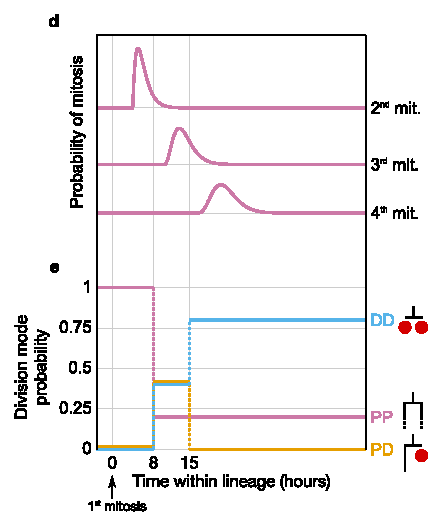
\includegraphics{3de}\caption{\label{fig:zf-model}\textbf{Upper}: The probabilities in the model
for the second, third, and fourth mitosis within a lineage to occur,
measured against the first mitosis. \textbf{Lower}: The time-dependent
probabilities for modes of division of RPCs in the model.}
\end{figure}


Thus, to fully define the model, we only have to specify two time
points to delineate the intermediate PD phase and the probabilities
within that phase. The times were chosen to be 8 hr and 15 hr after
the first mitosis, which essentially straddle the subsequent bursts
of mitoses; it was found that the outcome was not particularly sensitive
to the precise timing in any case, as long as they did not significantly
reassign mitosis to be in different phases. The proportion of PP divisions
was chosen, for simplicity again, to be the same as the terminal phase,
i.e., one in five. The final parameter, the probability for PD divisions,
was chosen to give the correct average size of 72 hpf clones induced
at 24 hpf, which corresponded to two in five divisions. The proportion
of DD is thus two in five during this intermediate phase.This model
was implemented as a custom-written Monte Carlo simulation, which
outputs probabilities for observing clones of different sizes. While
a comparison of the measured clone size distribution to the model
reveals a favorable fit to the experimental data (\figref{zf-model-comparison}),
the freedom to adjust control parameters limits its credibility. Fortunately,
we can make use of the live-imaging data to challenge some of the
assumptions and predictions of the model, below.

\begin{figure}
\centering{}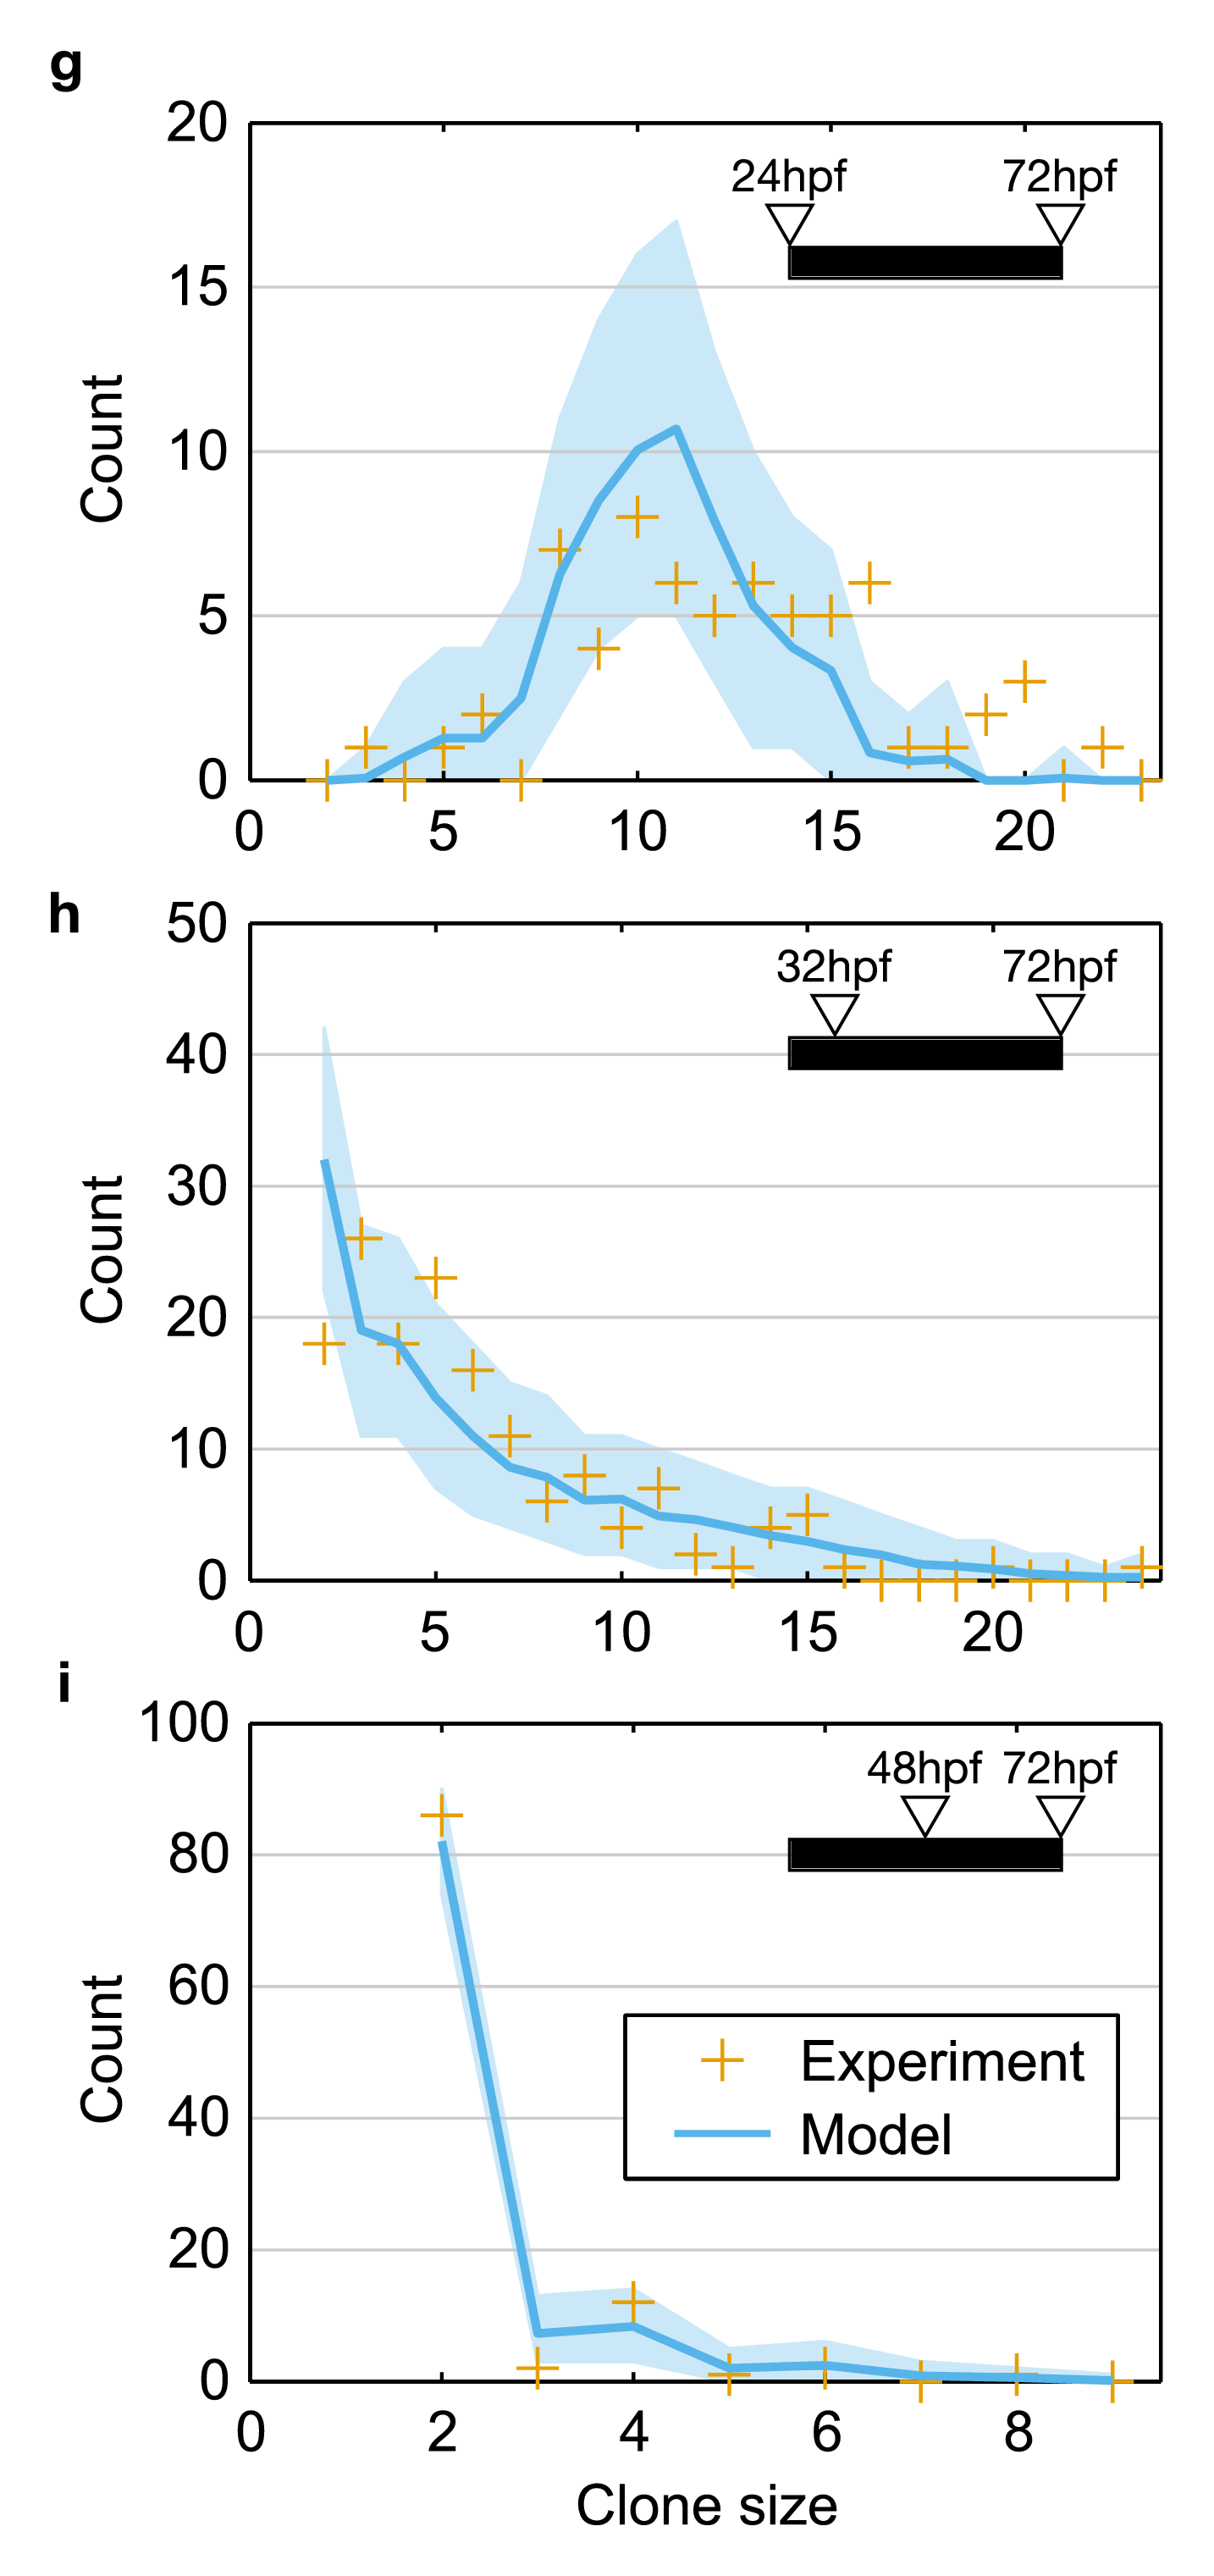
\includegraphics{3ghi}\caption{\label{fig:zf-model-comparison}Shows fits between model predictions
(cyan lines with shaded blue regions show 95\% plausible intervals
due to finite sampling) and size distributions (orange crosses) of
clones induced at 24 hpf (left), 32 hpf (middle), and 48 hpf (right).}
\end{figure}



\section{Live Imaging of Clones and Histogenesis}

In limited cases, by time lapse imaging, it is possible to reconstruct
the entire lineage tree (\figref{zf-lineage-trees}). Amazingly, almost
all the features deduced from clonal can be observed, such as PP divisions
following PD divisions, and the near synchronous sister divisions
(fig). An unexpected feature is a variation of cell cycle length depending
on fate outcome; in particular, PP and PD divisions are narrowly distributed
around a similar average of 7.5 \textpm{} 1.3 hr, but terminal DD-type
divisions have cell cycle times of 12.1 \textpm{} 1.0 hr. 

\begin{figure}
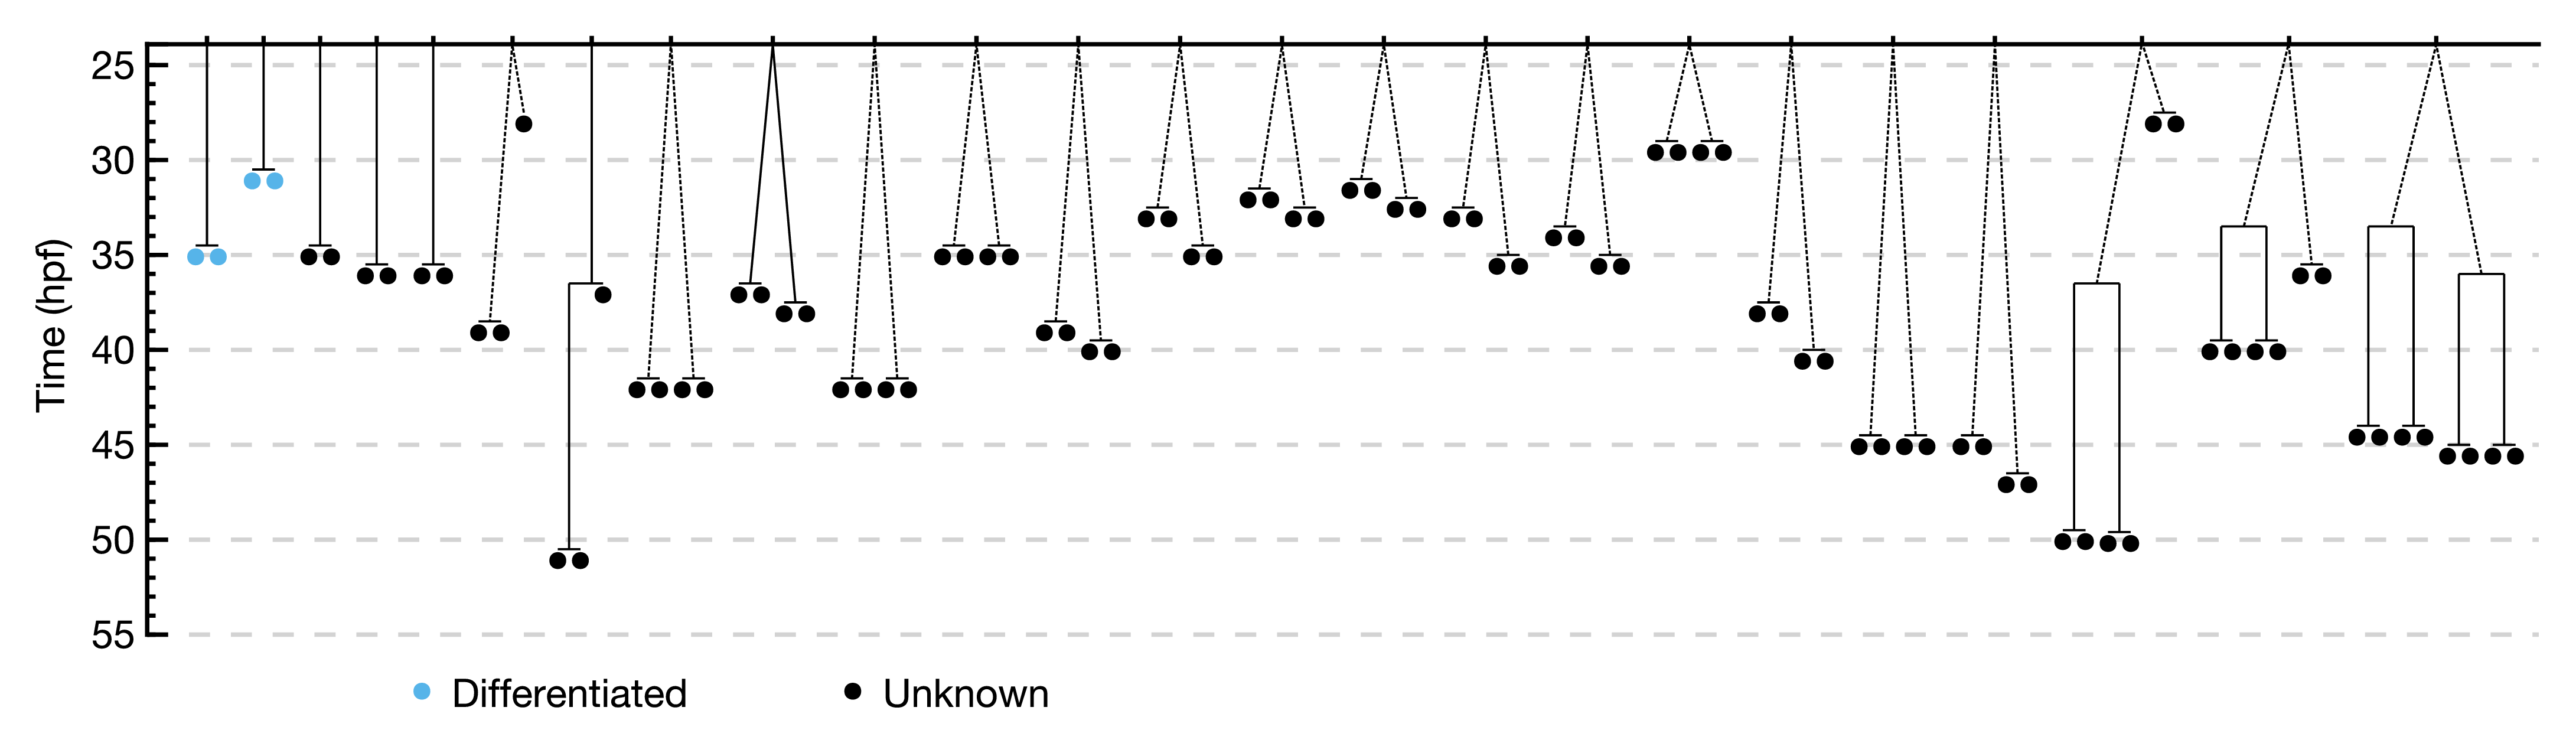
\includegraphics[width=1\textwidth]{live-24h}

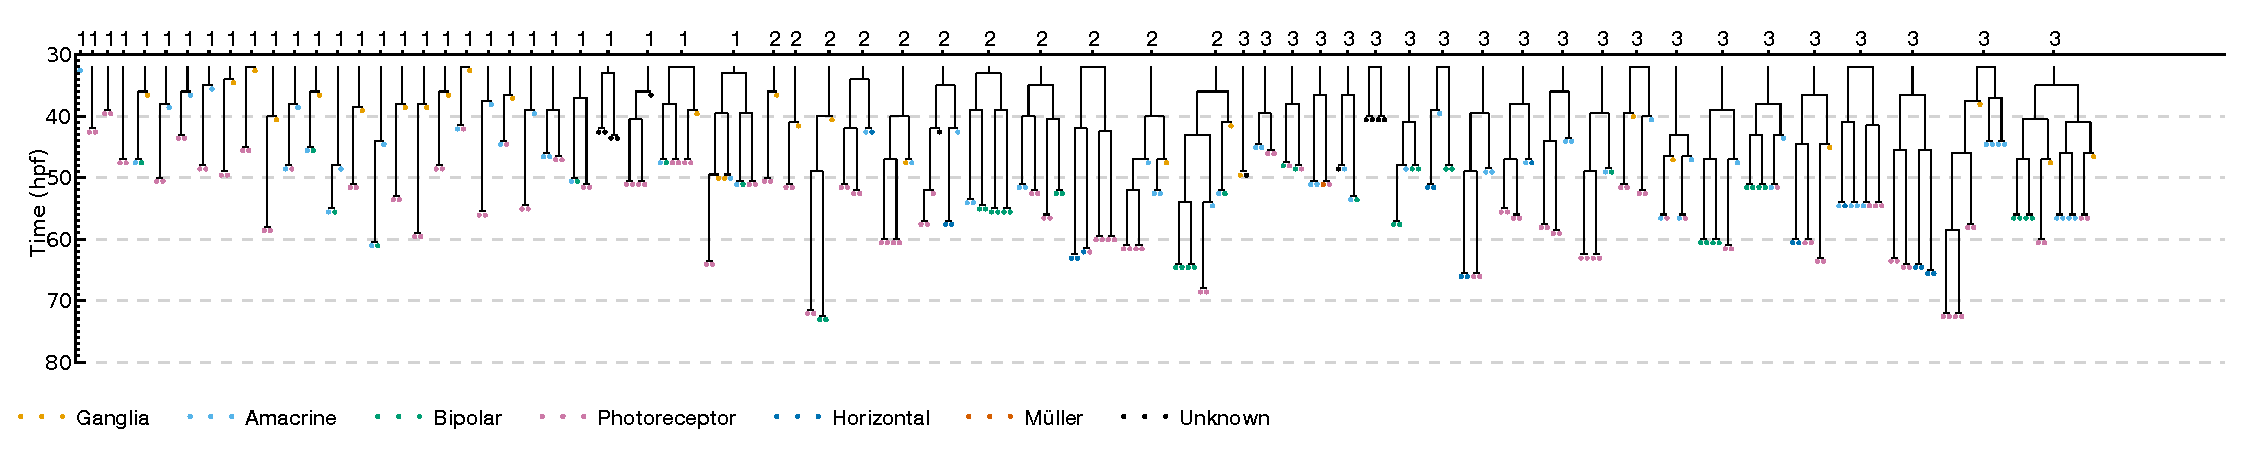
\includegraphics[width=1\textwidth]{live-image-trees}

\caption{\label{fig:zf-lineage-trees}\textbf{Upper: }Reconstructed lineage
trees from progenitors at 24 hpf, imaged at 48 hpf. Most cells have
yet to differentiate, so whilst almost certainly progenitors, we cannot
be certain. \textbf{Lower}: Reconstructed lineage trees from 60 photoconverted
progenitors at 32 hpf, imaged at 72 hpf. The numbers across the top
indicate the rough spatial location of the progenitor, nasal (1),
middle (2) or temporal (3).}
\end{figure}


The reconstructed lineage trees also offer an unprecedented view on
how histogenesis occurs, i.e. how some cell types are born before
others. At the population level, there is overlap leading to several
cells types being generated at the same time (fig). We seek here to
distinguish between simple overlap of strictly defined ordering within
each lineage, and where ordering is loosely defined within individual
lineage trees. We find that in DD divisions, almost all possible pairs
of cell types occur (fig). This eliminates the possibility of stereotypical
succession of cell types, however, it does not satisfactorily explain
the observed histogenesis. To attempt an answer, we performed a qualitative
analysis of the available data, by trying to compare the clone composition
of sister RPCs. In particular, we compress each subclone from a tree
into a string (represented graphically as a bitmap in \figref{zf-barcode},
left) and compare strings by a standard Levenshtein distance measure
(which counts the number of single-character edits that would be necessary
to turn one string into another). Finally, we use a standard hierarchical
clustering algorithm to sort the strings according to their similarity.
It was important to compare not only the final cell types generated
by each lineage but also the structure and order in which the cells
appear. To do this, we chose a particular representation of trees
as strings in order to preserve the tree structure. Specifically,
we embedded each tree into a complete tree of sufficient depth, then
performed a depth-first traversal to gather the cell types into a
string (\figref{zf-barcode}, left). \figref{zf-barcode}, right,
shows the subclones from the live-imaging data (with hierarchical
similarity shown as a tree at the bottom and sister lineage relation
at the top). We can discern no significant patterns from this data.

\begin{figure}
\begin{centering}
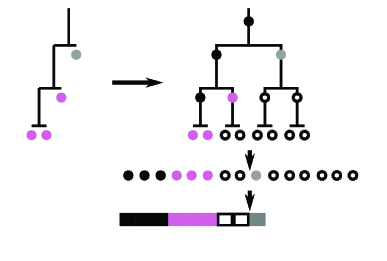
\includegraphics[width=0.4\textwidth]{zf-barcode}
\par\end{centering}

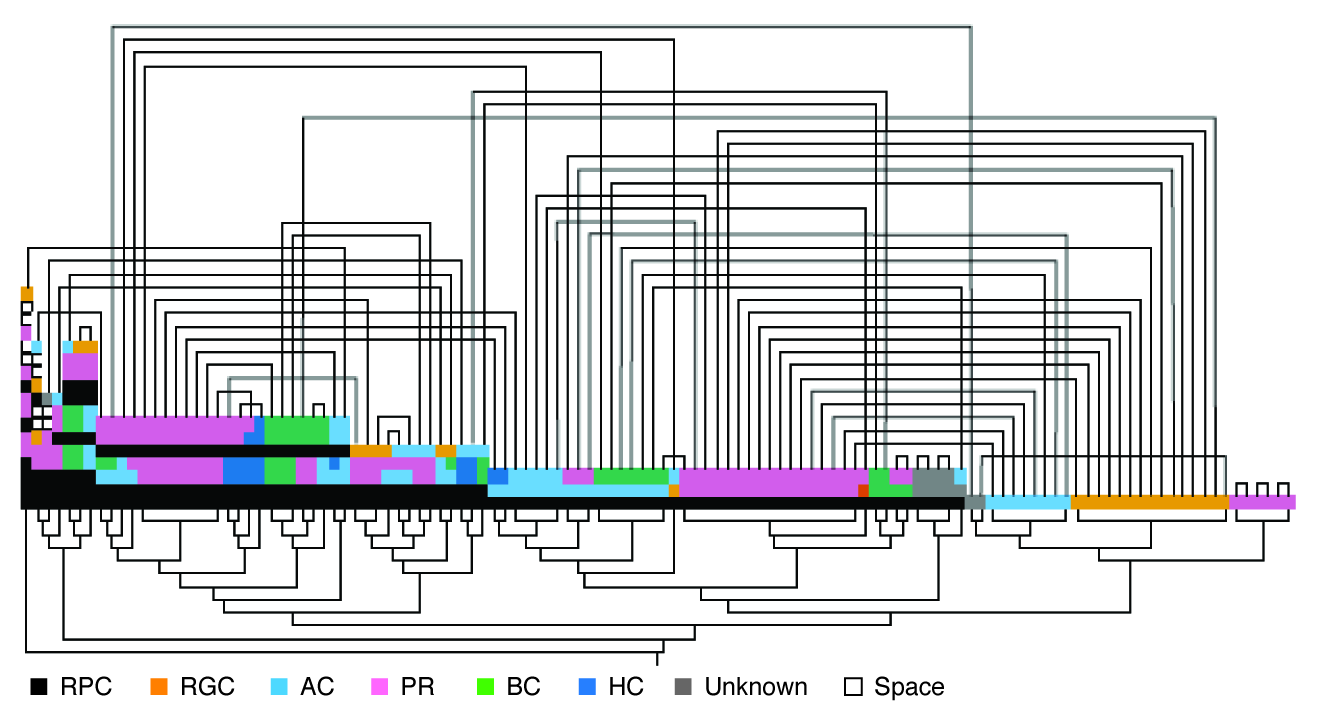
\includegraphics[width=1\textwidth]{zf-cluster-analysis}

\caption{\label{fig:zf-barcode}\textbf{Upper}: Illustration of compressing
of single lineage tree into a barcode. \textbf{Lower}: Barcode cluster
analysis of clones from \figref{zf-lineage-trees} split into sister
lineages (connected above), embedded into the smallest symmetric tree
(inserting space as necessary), and converted into a barcode by a
depth-first traversal to preserve structural units and hierarchically
clustered according to Levenshtein distance (shown by the tree below).
While sisters show similar sizes (due to their being born at the same
time and place), there are no other obvious correlations between sister
lineages.}


\end{figure}



\section{Discussion}

In summary, based on clonal analysis, we constructed a model for zebrafish
retinal development, of independent progenitors carrying out a stochastic
program, with evolving probabilities determined by their space-time
location in a simple fashion. We verified the model with detailed,
though limited, lineage trees obtained by live imaging studies. Although
the model explains the fate choice of progenitors and the clone sizes
observed, it does not satisfactorily explain the cell type choice
and observed histogenesis. The publish work {[}cite{]} includes a
further experiment dissecting a possible link between asymmetric divisions
and production of ganglial cells, but the conclusions are somewhat
preliminary. 


\chapter{Conclusion}

\bibliographystyle{apsrev4-1}
\bibliography{everything}

\end{document}
